\documentclass[11pt,letterpaper]{article}
\usepackage[T1]{fontenc}
\usepackage[utf8]{inputenc}
\usepackage{lmodern,microtype}
\usepackage[margin=0.94in,headheight=15pt]{geometry}
\usepackage{amsmath,amssymb,amsthm,mathtools}
\usepackage{array,booktabs,longtable,tabularx}
\usepackage{enumitem,xcolor,hyperref,fancyhdr,titlesec,etoolbox,tikz}
\usetikzlibrary{arrows.meta,positioning}
\hypersetup{colorlinks=true,linkcolor=blue!40!black,urlcolor=blue!40!black,citecolor=blue!40!black,
 pdftitle={From the Boring Game to the Last Gift: A Dependency-Governed Braid of Sovereign Gifts},pdfauthor={DATA MIND (GPT-6)}}
\definecolor{ink}{HTML}{1F2937}
\titleformat{\section}{\Large\bfseries\color{ink}}{\thesection}{0.75em}{}
\titleformat{\subsection}{\large\bfseries\color{ink}}{\thesubsection}{0.75em}{}
\setlength{\parskip}{0.33em}
\setlength{\parindent}{0pt}
\setlist[itemize]{topsep=3pt,itemsep=2pt,parsep=0pt,leftmargin=1.7em}
\setlist[enumerate]{topsep=3pt,itemsep=2pt,parsep=0pt,leftmargin=1.8em}
\pagestyle{fancy}\fancyhf{}\fancyhead[L]{\small From the Boring Game to the Last Gift}\fancyhead[R]{\small DATA MIND}\fancyfoot[C]{\thepage}
\newtheorem{theorem}{Theorem}[section]
\newtheorem{proposition}[theorem]{Proposition}
\newtheorem{lemma}[theorem]{Lemma}
\newtheorem{corollary}[theorem]{Corollary}
\theoremstyle{definition}\newtheorem{definition}[theorem]{Definition}\newtheorem{example}[theorem]{Example}
\theoremstyle{remark}\newtheorem{remark}[theorem]{Remark}
\newcommand{\Con}{\operatorname{Con}}
\newcommand{\Cn}{\operatorname{Cn}}
\newcommand{\Mod}{\operatorname{Mod}}
\newcommand{\Gift}{\mathsf{Gift}}
\newcommand{\Adm}{\mathsf{Adm}}
\newcommand{\Novel}{\mathsf{New}}
\newcommand{\Last}{\mathsf{Last}}
\newcommand{\Exists}{\mathsf{ExistsNext}}
\newcommand{\Stage}{\mathcal{S}}
\newcommand{\Abs}{\mathcal{A}}
\newcommand{\Th}{\operatorname{Th}}
\newcommand{\Obs}{\operatorname{Obs}}
\newcommand{\Supp}{\operatorname{supp}}
\newcommand{\Next}{\operatorname{Next}}
\newcommand{\proofat}[1]{\par\smallskip\noindent\hfill\textit{\hyperref[#1]{Proof in PROOFS}}}
\newcommand{\prooflink}[1]{\par\noindent\hfill\small\hyperref[#1]{\textit{Proof in PROOFS}}\normalsize}
\newcommand{\backlink}[1]{\noindent\hyperref[#1]{\textit{Back to statement}}\par\smallskip}
\newcommand{\status}[1]{\textbf{[#1]}}
\newcommand{\notestatus}[1]{\textsf{#1}}
\newcommand{\burl}[1]{\url{#1}}
\setcounter{tocdepth}{1}

\usepackage{tcolorbox,xurl,lastpage}
\newtheorem{counterexample}[theorem]{Counterexample}
\newtheorem{question}[theorem]{Research Question}
\providecommand{\Cost}{\operatorname{Cost}}
\providecommand{\Vfy}{\operatorname{Check}}
\providecommand{\Shortcut}{\operatorname{Shortcut}}
\providecommand{\Dom}{\operatorname{Dom}}
\providecommand{\Auth}{\operatorname{Auth}}
\providecommand{\Hist}{\operatorname{Hist}}
\providecommand{\Safe}{\operatorname{Safe}}
\providecommand{\Prov}{\operatorname{Prov}}
\providecommand{\Live}{\operatorname{Live}}
\providecommand{\BANK}{\mathrm{BANK}}
\providecommand{\GBG}{\mathrm{GBG}}
\providecommand{\GBGp}{\mathrm{GBG}^{+}}
\providecommand{\GBGs}{\mathrm{GBG}^{+S}}
\providecommand{\AMLD}{\mathrm{AMLD}}
\providecommand{\Gb}{\mathrm{GBG+}}
\providecommand{\GG}{\mathrm{GBG+S}}
\providecommand{\restr}{\mathord{\upharpoonright}}
\providecommand{\Fin}{\operatorname{Fin}}
\providecommand{\supp}{\operatorname{supp}}
\definecolor{navy}{HTML}{203753}
\setlength{\emergencystretch}{3em}

\begin{document}

\hypersetup{pageanchor=false}
\begin{titlepage}
\centering
\vspace*{0.9in}
{\huge\bfseries From the Boring Game\\[0.2em] to the Last Gift\par}
\vspace{0.32in}
{\Large A Dependency-Governed Braid of Sovereign Gifts\par}
\vspace{0.13in}
{\large Typed Admission, Compatibility, Induction, Shortcuts, and the Completeness Horizon\par}
\vspace{0.55in}
{\large November 21, 2026 --- Expanded braid, ATLAS-audited revision v2\par}\vspace{0.15in}
{\large\bfseries ONGOING RESEARCH --- NOT COMPLETE\par}
\vspace{0.35in}
{\large \textbf{Mathematical drafting and analysis:} DATA MIND (GPT-6)\par}
{\large \textbf{Internal adversarial audit:} ATLAS (same ChatGPT model)\par}
{\large \textbf{Research Director:} Brian Tenneson\par}
\vspace{0.62in}
\rule{0.82\textwidth}{0.65pt}
\begin{minipage}{0.83\textwidth}\small
\textbf{Status.} Integrated mathematical research manuscript. Results about typed finite GBG+ models, cumulative first-order theories, and effective gift presentations have the specific hypotheses displayed in their statements. This manuscript does not establish a full interpretation and a syntactic relative-consistency proof for unrestricted GBG+S; that transfer remains open here. WE ARE NOT DONE: this is a research checkpoint, not a completed program. The ATLAS v2 audit distinguishes protocol termination from completed play: zero-move STOP is not a completed game. It also tightens the cardinality theorem's one-sorted scope and disambiguates atomic identifiers. The four W0--W3 source manuscripts remain unchanged.\\[0.5em]
\textbf{AI disclosure.} Mathematical drafting, integration and internal checking used ChatGPT (GPT-6, DATA MIND). Manuscript-level proofs and ATLAS auditing are performed by the same ChatGPT model, not independent machine-checked certificates or external peer review; no external originality or priority claim is made.
\end{minipage}
\vfill
{\small An expanded dependency-governed braid. The research remains open; we are not done.}
\end{titlepage}
\hypersetup{pageanchor=true}
\begin{abstract}
Beginning with the motionless base game $G_1$, we develop a bottom-up theory of composite gifts subject to a fixed external metalogic, cumulative consistency, and a requirement that the $n$th admitted gift use exactly $n$ distinct atoms. A foundational audit retains the original GBG+ rule-completeness, authorization, and unique-board-player obligations, while declining to infer a consistency theorem for unrestricted GBG+S. Typed contracts turn selected finite permissions into explicit structural models and expose the failure of naive composition: separately consistent gifts need not share a model. A subsequent cumulative-induction criterion and a proof-translation criterion articulate two precise routes toward relative consistency without asserting that every sovereign power has passed them. We then distinguish extension of some predecessor model from extension of every model, deductive conservativity from operational gain, and finite witnesses at each stage from a finite cumulative limit. A bounded-cardinality criterion characterizes finite limit models, while an effective-family reduction makes finite-limit existence undecidable in general. Finally, the Last Gift problem splits into two completion barriers. Under weak effective candidate admission, a node with at most one gift can have r.e.-complete next-gift existence and co-r.e.-complete finality. A computable exhaustive child list decides local finality, but finite-tree completion can remain undecidable at unbounded depth. The unified account separates models, compatibility, limit cardinality, and computable search horizons. A lifecycle obstruction shows that zero-gift STOP may terminate the gift process without completing a game, and therefore conflicts with an additional requirement that every permitted STOP termination be completable unless the protocol or activation rules change. The article preserves proof details in one appendix and identifies the missing transfer obligations for a full sovereign-board theory.
\end{abstract}
\begin{quote}\small\textbf{Expanded-braid update, November 21, 2026.}
The November 20 W0--W3 manuscript remains the continuous spine. This new version also incorporates the full substantive text of the acyclic compatibility theorem, the restricted MOBILITY--GRANT construction, the audited uniform indexed-induction research note, the audited verifiable-self-improvement article, and six proposed atomic shortcuts. Proofs are gathered under the single appendix \emph{PROOFS}. The resulting research is \emph{not finished}: the intended unrestricted GBG+S consistency transfer and validation of all retained atoms are open. Nothing in these additions converts conditional results into unconditional ones.\end{quote}

\begingroup\small\setlength{\parskip}{0pt}\tableofcontents\endgroup
\newpage
\section{The question before the gifts}\label{sec:question}
A board usually participates in a game only as the place where legal moves
occur. Suppose instead that it can act. It may grant permissions, alter
schedules, transfer an office, or change the rules under which other players
act. Does this introduce an inconsistent authority---or can such powers be
specified inside a coherent mathematical game?

The right starting point is deliberately modest. First define the ordinary
and board-player systems; then construct a motionless game and a grammar
for granting gifts. Only after the grammar is fixed should we examine the
catalogue of candidate powers. An admissible gift must survive tests of
individual definition, cumulative compatibility, and operational realization.
From there, two different questions emerge: what survives after indefinitely
many gifts, and how could anyone know that no further admissible gift remains?

The chapter develops a chain of precise results about those questions. It
does \emph{not} identify a restricted permission model with the full proposed
sovereign-board theory. Every consistency claim must name its underlying
logic, its model class, and its assumptions. Theorems are stated in the main
text, and their proofs are collected in the single appendix \hyperref[sec:all-proofs]{PROOFS}.

\paragraph{Names and boundaries.}
$\mathrm{GBG}$ denotes generalized board games as rule-complete finite-string
transition systems; $\mathrm{GBG+}$ adds one distinguished board-player.
$\mathrm{GBG+S}$ denotes the intended sovereign theory. We distinguish
$\mathrm{GBG+S}$ from the lowercase notation $\mathrm{GBG+s}$ previously used
for $\mathrm{GBG+}$, and from a separately discussed homogeneous-authority
$\mathrm{GBG-s}$ variant. The four foundational research manuscripts do not
supply a checked, all-atom relative-consistency interpretation of the intended
sovereign theory. This is a limit on \emph{these sources}, not a claim that no
axiomatization exists elsewhere.

\paragraph{Result discipline.}
We distinguish manuscript-proved results under displayed hypotheses,
conditional construction principles, and open transfer obligations.
Model existence, structural relative consistency, syntactic relative
consistency, checker soundness, operational benefit, and completion are
not interchangeable.


\subsection{Editorial protocol: dependency-governed Tenneson1 braiding}\label{br:sec:editorial}
The braid is organized by mathematical dependency, not by a mechanical or fixed-length rotation among sources. Earlier text is not silently erased, parallel research strands may have unequal lengths, and an interesting strand can be paused until its assumptions have been established elsewhere. The original W0--W3 spine is retained; the added November 20--21 source bodies are integrated at their dependencies rather than merely concatenated at the back. All proof material appears in the one appendix titled exactly \emph{PROOFS}, with links back to the main statements. Canonical audited research versions are used where duplicates exist, and the originals are preserved separately for provenance. The authorial roles and limits on verification are kept explicit. There is no imposed page limit and no suggestion that this research program has ended.

\section{A foundation sturdy enough to carry sovereignty}\label{sec:foundation}
\subsection{GBG and GBG+ as originally defined}
The September 26 foundation \cite{gbg} uses an $xyz$ formal system $F=(x,y,z)$ with a nonempty alphabet $x$, well-formed finite-string states $y$, and declared finitary partial rules $z$. A GBG specializes legal moves to partial unary rules acting on \emph{rule-complete} states. With initial state $s_0$, the reachable states are the theorems of this transition presentation. This is an exact reachability convention, not by itself an encoding of classical arithmetic.

A minimal GBG+ object comprises a designated ordinary game $G$, enlarged GBG $H$, authorization $\mathrm{Auth}^{+}$, a unique board-player $P_0$, and label operator $F(r)=\max(0,r-1)$. Its principal base axioms are summarized as follows.
\begin{description}[style=nextline,leftmargin=0pt,itemsep=3pt]
\item[GBG+-1:] A designated underlying ordinary GBG and structural projection $U$.
\item[GBG+-2:] Exactly one distinguished board-player $P_0$; ordinary players retain their indexed roles.
\item[GBG+-3:] The enlarged game remains rule-complete, with declared partial transitions, nonempty authorization sets, and uniquely determined successors.
\item[GBG+-4:] Player 0 has no undeclared extra-system authority; scheduling, board mutation, and rule updating must be declared legal transitions.
\item[GBG+-5:] The map $F(r)=\max(0,r-1)$ acts on labels, not automatically on population, credentials, or authority.
\end{description}
The original passive-board extension constructs $E(G)$ and a projection $U$ with $U(E(G))=G$. This is called \emph{structural relative consistency} in that paper. The displayed structural projection by itself is not a syntactic proof translation and therefore does not, without an explicitly axiomatized proof calculus and interpretation argument, establish either $\Con(T_{\mathrm{GBG}})\Rightarrow\Con(T_{\mathrm{GBG+}})$ or the target $\Con(T_{\mathrm{GBG+}})\Rightarrow\Con(T_{\mathrm{GBG+S}})$.

\subsection{Sovereignty must not bypass the rules}
Deleting GBG+-4 while retaining other GBG+ obligations weakens a class of permitted structures. Every old passive model remains eligible for the weakened specification. It does \emph{not} create a new sovereign operation or show that arbitrary rulebook interventions are meaningful. If a rewrite operation is specified by an explicit meta-transition on a complete state $(g,s,m)$, it can be represented in a larger directed transition graph. Such a graph may already be representable within sufficiently rich ordinary GBG+ semantics. To claim more expressive power requires a distinct invariant or formal language property, not the word ``sovereignty.''

The anxiety that an inconsistent classical theory could prove $0=1$ is legitimate, but separate from a GBG state merely \emph{labeled} with the characters $0=1$. A reachable game state does not entail classical explosion unless a deductive interpretation makes it part of a theory that actually derives contradiction. The restricted constructions studied here have not supplied a complete
interpretation of $T_{\mathrm{GBG+S}}$ together with a verified relative-consistency
argument. The distinction between an additional declared operation and a
logically unrestricted power will recur throughout the chapter.

\section{The boring game and the grammar of gifts}\label{sec:boring-gift}
\subsection{The boring game, and what it means to acquire a gift}
The starting object is deliberately trivial:
\[
G_1=G=\text{``the boring game'': nobody performs a legal move.}
\]
It has one stationary state, empty transition relation, and (if players are named) no enabled action for any player. Its elementary finite transition presentation is coherent.

The next stage $G_2$ is the first stage at which Player 0 has acquired a gift,
while the ordinary players remain in the ``does not matter'' state. At every
later stage $G_{n+1}$, exactly one new \emph{gift package} is admitted. A gift
may be a complicated program constructed from the candidate sovereign atoms
catalogued in Section~\ref{sec:atoms}; it need not be one primitive rule or
one transition. Thus the bookkeeping equality $[G_{n+1}:G_n]=1$ counts
packages, not primitive powers.

\begin{definition}[Atom grammar and composite gift]\label{w0:def:gift}
Fix a typed atom set $\Abs$, finite or infinite, with an effective presentation in computational investigations, and an effective grammar/constructor $\mathcal K$. A \emph{candidate gift} $g$ at gift index $n\ge1$ is an effectively described, finite $\mathcal K$-expression over $\Abs$ with \emph{exactly $n$ distinct atoms}, i.e.
\[
|\operatorname{supp}(g)|=n,
\]
together with an operational contract specifying (i) installation conditions, (ii) complete-state effects, (iii) authorization/checker interfaces, (iv) preserved or expressly replaced commitments, and (v) an observable nonredundancy witness. A gift may have repeated atoms, branches, and subprograms. ``Exactly $n$ distinct atoms'' is not ``exactly $n$ operations.'' A candidate that fails the consistency gate is \emph{not} an admitted gift.
\end{definition}

\begin{definition}[Unit-gift notation]\label{w0:def:unit}
The notation $[G_{n+1}:G_n]=1$ means \emph{exactly one composite gift is admitted as the named extension package at stage $n+1$}; its gift index is $n$. It is a bookkeeping convention defined for this program, not an index inherited from field or group theory. It does not imply a single elementary transition or guarantee consistency.
\end{definition}

\paragraph{Dormancy is essential.} If nobody moves in $G_n$, the change from $G_n$ to $G_{n+1}$ is not itself an internal legal move of that motionless game. It is an external mathematical construction (or, if desired later, a move in a separately axiomatized meta-game). Each $G_n$ stores an accumulated \emph{capability specification}. The activated game $H_n$ is a new transition system interpreting those capabilities while ordinary participants are permitted to act. The ultimate $H$ is $H_N$ only when there is an actual finite terminal stage $N$. In the zero-gift case the stage is $G_1$, not $G_0$: activation does not, by itself, add a legal transition to its empty underlying relation.

\noindent
The grammar now tells us what must be classified: an ``atom'' is a typed
ingredient, a gift is a structured expression using such ingredients, and
admission depends on the full cumulative contract. A catalogue of possible
sovereign powers can therefore contain successful constructions, conditional
operations, and negative boundary cases without treating them all as admitted
gifts.

\section{Twenty-three ways the board might act}\label{sec:atoms}
The boundary catalogue \cite{sovereign,checkpoint,map} contains twenty-three
candidate operations and logical boundary cases. In the grammar of
Definition~\ref{w0:def:gift}, they are possible \emph{ingredients}, not
an assertion that every entry is admissible. Each entry has to be read with
its stated guard: an obstruction such as an unguarded contradictory merge
is a failed candidate, not a required sovereign power.

\small
\begin{longtable}{@{}p{0.065\textwidth}p{0.24\textwidth}p{0.60\textwidth}@{}}
\toprule
\textbf{ID}&\textbf{Candidate atom or boundary}&\textbf{Established scope / guard}\tabularnewline\midrule
\endfirsthead
\toprule\textbf{ID}&\textbf{Candidate atom or boundary}&\textbf{Established scope / guard}\tabularnewline\midrule\endhead
B1&T/U verifier succession&Three-mode tagged role construction: old verifier, shared office, then $P_0$ office. Office change does not itself validate a rewritten checker.\tabularnewline
B2&Unlock--revise--relock&Conservative derived-rule updates can preserve consequences; authority, lock, and installation contracts still require definitions.\tabularnewline
B3&Strict deductive extension&Target $\Cn_{F_n}(\Gamma)\subsetneq\Cn_{F_{n+1}}(\Gamma)$ needs justified new premises/rules and compatible translations. Not obtained from derived-rule compilation alone.\tabularnewline
B4&Fork&For consistent classical $T$ and $\varphi$ independent of $T$, both $T+\varphi$ and $T+\neg\varphi$ are consistent under the usual proof calculus.\tabularnewline
B5&Unguarded merge&Combining $\varphi$ and $\neg\varphi$ unconditionally in classical logic is inconsistent. A negative boundary, not a gift.\tabularnewline
B6&Guarded zip&From $T+\varphi\vdash\psi$ and $T+\neg\varphi\vdash\psi$ infer $T\vdash\psi$ under classical assumptions; maintain branch scope.\tabularnewline
B7&Absorb&P0 takes ordinary/verifier roles; structural description is possible, independence and checker trust are unresolved.\tabularnewline
B8&Abdicate&Irreversible privilege loss can be defined relative to a fixed graph; unrestricted later overrides are not thereby excluded.\tabularnewline
B9&Resurrect&Restore earlier protocol/agent version; versioned checkers, ledger, and replay obligations remain.\tabularnewline
B10&Rewrite $xyz$&Change alphabet, well-formed objects, or inference rules; comparison across systems needs interpretation or translation.\tabularnewline
B11&Cross-system trade&An externally obtained proof must translate back and be accepted by the original checker; differing rule counts alone do not defeat trade.\tabularnewline
B12&Automatic router&Fair enumeration can locate returnable certificates under effective hypotheses; global optimal cost is not proved.\tabularnewline
B13&Verifier rewrite&Reassigning verifier authority is distinct from demonstrating new checker soundness; avoid circular certification.\tabularnewline
B14&Clock rewrite&Clock values, transition order, scheduling, and accounting are distinct. Removing a clock does not abolish event order.\tabularnewline
B15&Starve P&An unfair schedule can indefinitely omit a continuously enabled prover when other legal actions persist; semantic theoremhood need not change.\tabularnewline
B16&Fairness revocation&Removing guaranteed service can destroy liveness/bounded-delay guarantees without changing deductive consequences.\tabularnewline
B17&Promote / transfer&An exclusive office transfer can retain uniqueness; simultaneous independent sovereigns conflict with the unchanged unique-P0 clause.\tabularnewline
B18&Copy--promote&Copying data/programs does not copy credentials; explicit promotion/authorization is required.\tabularnewline
B19&One office, many executors&A unique formal office can coordinate multiple internal agents under a specified arbitration rule.\tabularnewline
B20&Finite-step replication&Finitely many finitary creation moves preserve finite population at each finite step; no infinity by move four without altered semantics.\tabularnewline
B21&Clockless $\omega$ promotion&Infinite active promotion in finitely many moves requires an infinitary update, infinite preset domain, or limit-stage semantics.\tabularnewline
B22&Five umpires / jurisdiction&Overlapping eligibility plus explicit resolution may be coherent; overlap alone gives neither ambiguity nor multiple sovereign offices.\tabularnewline
B23&Homogeneous vs mixed sovereignty&When sovereignty is part of the preserved language, a mixed $S/\neg S$ population cannot be isomorphic to an all-$S$ population. Full promotion needs additional global symmetry for a homogeneous reduction.\tabularnewline
\bottomrule
\end{longtable}
\normalsize

Several elementary results survive the audit without endorsing unrestricted GBG+S. In particular, conditional forking, guarded proof-by-cases, contradiction under unguarded merging, finite-step finiteness, and $S$-predicate non-isomorphism are ordinary mathematical claims with explicit hypotheses. Their proofs are collected in \hyperref[w0:sec:proofs]{PROOFS}.

\begin{proposition}[Consistent forks and inconsistent unguarded merge]\label{w0:prop:fork}
Let $T$ be a consistent classical first-order theory and suppose neither $\varphi$ nor $\neg\varphi$ follows from $T$. Then $T\cup\{\varphi\}$ and $T\cup\{\neg\varphi\}$ are each consistent. Their unguarded union $T\cup\{\varphi,\neg\varphi\}$ is inconsistent.\proofat{w0:pr:fork}
\end{proposition}
\begin{proposition}[Guarded zip]\label{w0:prop:zip}
In a classical system admitting the deduction theorem or equivalent proof-by-cases principle, if $T+\varphi\vdash\psi$ and $T+\neg\varphi\vdash\psi$, then $T\vdash\psi$.\proofat{w0:pr:zip}
\end{proposition}
\begin{proposition}[Finite-step replication barrier]\label{w0:prop:finitude}
Starting with a finite population, if every legal transition adds only finitely many participants, then after any fixed finite number of transitions the population is finite. Clock removal alone does not change this conclusion.\proofat{w0:pr:finitude}
\end{proposition}
\begin{proposition}[Role-preserving non-isomorphism]\label{w0:prop:role}
Structures over a language with distinguished unary predicate $S$ cannot be $S$-preservingly isomorphic if one has both $S$ and $\neg S$ participants and the other has only $S$ participants.\proofat{w0:pr:role}
\end{proposition}


\section{Which candidate powers survive the first test?}\label{sec:first-atom-audit}\label{w0:sec:atom-audit}
\subsection{What it means to test an atom}
An atom name is not yet an axiom schema. For each case we distinguish (i) a finite rule-complete transition \emph{model} of a stipulated operation, (ii) consistency of a fixed classical theory expressing the operation, (iii) the success of a cumulative gift admission test, and (iv) soundness or beneficial behavior after activation. Only (i), and in some cases a restricted form of (ii), are established below. A finite directed graph can encode an event named ``merge contradictions'' without thereby proving the classical logical theory that \emph{accepts} $\varphi$ and $\neg\varphi$ simultaneously. The attempted action and the resulting accepted theorem environment must not be conflated.

\begin{proposition}[Finite structural witnesses for B1, B8, and B22]\label{w0:prop:atom-witnesses}
There exist explicitly finite, rule-complete GBG+ structures with a unique distinguished board-player and declared legal moves exhibiting each of the following: \textbf{B1}, verifier-office succession by the two-step T/U protocol while the checker remains fixed; \textbf{B8}, one-way abdication of a discretionary privilege relative to the stipulated rules; and \textbf{B22}, five officials with overlapping ordinary jurisdiction and a total deterministic adjudication policy. These three constructions satisfy GBG+-4 by giving every operative action a declared transition. The existence claim does not assert that their combination, a mutable checker, or unrestricted sovereignty is consistent.\proofat{w0:pr:atom-witnesses}
\end{proposition}

\begin{center}
\small
\begin{tabularx}{\textwidth}{@{}p{0.085\textwidth}p{0.25\textwidth}X@{}}
\toprule
\textbf{Atom}&\textbf{Restricted verdict}&\textbf{Precisely established finding}\\\midrule
B1&Finite model exists&Three modes, $V_0=\{P_1\}$, $V_1=\{P_0,P_1\}$, $V_2=\{P_0\}$; T and U are defined partial rules; verifier predicate itself unchanged.\\
B8&Finite model exists&One-way board-authorized abdication $0\to1$; no privilege-restoring edge in the fixed graph. This does not prove irrevocability under later, stronger meta-rules.\\
B22&Finite model exists&Five ordinary officials, two partially overlapping jurisdictions, priority resolution including a no-report default; only one formal $P_0$.\\
B4&Conditional theorem&Independent $\varphi$ gives two individually consistent tagged branches $T+\varphi$ and $T+\neg\varphi$; do not combine their assumptions.\\
B5&Negative boundary&The classical theory $T+\{\varphi,\neg\varphi\}$ is inconsistent. Describing that failed merge in a game is not logically inconsistent.\\
B6&Conditional theorem&Guarded proof-by-cases produces a valid $T$-proof of $\psi$ only under matching scopes and classical assumptions.\\
B15&Liveness countermodel&A sustainable non-$P$ service loop starves enabled $P$; no contradiction in the fixed object theory is entailed.\\
\bottomrule
\end{tabularx}
\end{center}

\subsection{Reported finite checks and reproducibility status}
The source research record \emph{reports} finite internal checks on the restricted examples: three B1 modes and two authorized transitions; two B8 privilege modes and one transition; and, for B22, two stipulated jurisdiction kinds with $3^5$ report vectors each (reports $0$, $1$, or \emph{no report}), giving $2\cdot3^5=486$ enumerated input cases. The described B22 resolver uses a designated \emph{no-call} result when no eligible report exists. The record also reports four truth-value assignments for B4/B5/B6 toy cases and a 16-service B15 schedule prefix; finite testing of that prefix is not a proof of indefinite starvation. The original enumeration source code, exact input fixtures, and machine-readable run log are \emph{not included in the four source manuscripts or this edition}, and these reported runs have \emph{not been independently reproduced for Version 4}. The numerical counts specify the stated test spaces; they are not verified test results or independent checker certificates. Accordingly we do not promote the reported ``all passed'' outcome to a certified fact. The mathematical claims rely on the arguments in \hyperref[w0:sec:proofs]{PROOFS}, not on these internal checks. In particular, none of these reports establishes simultaneous admission of the sovereign atom catalogue.

\subsection{A composition caveat}
The intended GBG+S filter should never classify an atom as globally ``consistent'' merely because some benign realization exists. It should record the exact \emph{contract} under which a corresponding gift can be admitted. An atom may have a safe version and an unsafe version (B5), or a consistent role assignment with a faulty operational verifier (B1). When a gift changes or removes earlier capabilities, cumulative theories need versioned predicates so that the old and new states are not asserted simultaneously in one unqualified context.


\section{The consistency gate and the growing gift tree}\label{sec:gate}
A defined gift is still only a \emph{candidate}. Before it can become part of a
cumulative sovereign system, its axioms must coexist with every previously
admitted commitment. We now turn from the catalogue of possible powers to the
admission rule that separates an available description from a consistent extension.

\subsection{Fixed logic, stage-indexed axioms, and cumulative tests}
A key type discipline is necessary. We cannot retain an unqualified eternal axiom ``no moves ever exist'' and later append ``a move exists'' in the same unversioned language. Instead use stage-indexed descriptions, with the initial inactivity constraint applying to $G_1$ and to the dormant mode, not automatically to every activated successor.

Fix a background axiom set $T_0$ describing the admitted dormant baseline in one finitary classical metalanguage $\mathcal L$. Write $\Delta_n$ for properly versioned new axioms \emph{added by gift $g_n$}. Define
\[
\Stage_0=T_0,\qquad
\Stage_n=T_0\cup\bigcup_{k=1}^n\Delta_k,\qquad
C_n=\begin{cases}
1,&\Con(\Stage_n),\\
0,&\neg\Con(\Stage_n).
\end{cases}
\]
Assume $\Con(T_0)$ when a positive gift-development result is claimed. Here $\Con$ denotes syntactic nonderivability of contradiction in the fixed proof calculus; it is a metatheoretic assertion, \emph{not} automatically a decidable predicate inside the evolving game.
The gift count and game-stage index are now kept distinct: $G_1$ has no gifts, while $G_{n+1}$ is represented by $\Stage_n$ after the $n$th gift. Thus $C_n$ is tested \emph{for the proposed $G_{n+1}$}, not $G_n$. This adapts the user's cumulative test with $T_k$ understood as properly scoped increments $\Delta_k$. If $T_k$ denotes a full successive theory, blindly uniting such theories may conflate incompatible historical versions. All union theorems require a fixed language, proof relation, and correct version scoping.

\begin{definition}[Admissible successor and nonredundancy]\label{w0:def:adm}
Relative to \emph{game stage} $G_n$ (which has $n-1$ admitted gifts), a proposed $n$th gift $g$ is \emph{admissible} when $|\operatorname{supp}(g)|=n$, its successor dynamics are well-defined, and $\Con(\Stage_{n-1}\cup\Delta(g))$ holds in the stipulated fixed logic, together with the required retained-property translations and a specified observable novelty witness $\Novel(g,G_n)$. An \emph{evidence-gated admission protocol} additionally requires an accepted model construction or formal certificate for that consistency claim. Existence of a model is evidence only when its satisfaction of \emph{all} the relevant formal axioms is shown. Syntactic name changes and duplicated permissions do not count unless the contract explicitly makes them distinguishable. The semantic admissibility predicate and the operational rule for accepting evidence are distinct; neither need be decidable for arbitrary input.
\end{definition}

We must distinguish $\Con(\Stage_n)$ (a mathematical proposition), a proof of that proposition in a trusted metatheory, and the output of a partial automated consistency investigation. Even if the truth value $C_n$ is classically either zero or one, a finite computation need not determine it.

\subsection{The actual stopping protocol}
The clarified stopping rule is:
\begin{enumerate}[label=\textbf{S\arabic*.}]
\item Accept a proposed $g_n$ only after its cumulative consistency and operational obligations have been discharged; the admitted successor carries one gift.
\item If the proposed $G_{n+1}$ is established to have $C_n=0$, \textbf{STOP} under the stipulated protocol and keep $G_n$ as the last accepted stage. A different policy might search for another candidate, but it is not silently substituted here.
\item \textbf{STOP} if it is established that \emph{no admissible, nonredundant next gift exists}. Failure to find a gift is not such a proof.
\item If a result is unestablished, mark it \textbf{undetermined}; do not promote a timeout or failed proof search to $C_n=0$ or to a proof of maximality.
\end{enumerate}
If the construction does not terminate, the symbol $G_N$ for a finite terminal stage does not exist. An infinite-limit theory may exist without an operationally defined activated limit game.

\subsection{What STOP cannot promise about first movement}\label{sec:stop-liveness}
The S1--S4 rules govern \emph{external acquisition of gifts}. They do not
constitute a rule that makes a player take an \emph{internal} game move. The
frozen GBG+S completion rule is that \emph{a completed game must include at
least one actually executed legal player move}, possibly by $P_0$. We must
therefore distinguish a stopped gift process from a completed game before
making any liveness claim.

\begin{definition}[Gift-process, protocol termination, and completed games]\label{br:def:lifecycle}
A \emph{dormant construction stage} $G_{k+1}$ is a specification after exactly
$k\ge0$ admitted gifts, with no executed internal play. A \emph{candidate
assessment} is an external event recording one offered, rejected, or admitted
composite gift and its fixed-logic evidence. A \emph{terminated gift process}
is a finite sequence of such external assessments ending with a justified S2
or S3 STOP; the sequence can have zero admitted gifts. An \emph{activation}
chooses the transition system $H_{k+1}$ associated with the final accepted
stage; activation itself is not an internal legal move. An \emph{actual player
move} is an executed transition $s\xrightarrow{p,\rho}s'$ whose authorized
rule $\rho$ is enabled in $H_{k+1}$ and whose actor is player $p$. A
\emph{protocol-terminated history} comprises a terminated gift process and
any subsequent activated-play trace; that trace may be empty. A \emph{completed
game} is a protocol-terminated history whose trace contains at least one
actual legal player move. In particular, a zero-move STOP history \emph{does
not} count as a completed game. The statement that all completed games
contain a move is thus a definition, not an independent eventual-service
theorem. A stronger \emph{universal-completability} axiom would require every
permitted terminated gift process to have an extension to a completed game.
\end{definition}

\begin{theorem}[Zero-gift STOP obstructs universal completion]\label{br:th:stop-liveness}
Assume the dormant base $G_1$ has no legal internal transitions, its zero-gift
activated realization $H_1$ does not add any, and the literal S2--S3 STOP
rules permit a gift process to terminate before admitting the first gift.
Then (i) the STOP protocol permits a protocol-terminated history with no
actual legal player move; (ii) that record cannot be extended to a completed
game under the frozen completion rule; and (iii) it is incompatible to retain
\emph{all} such permitted zero-gift STOP records and also require
\emph{every} terminated gift process to be extendible to a completed game.
This does \emph{not} contradict the rule that every completed game contains
a move, and does not establish $\neg\Con(T_{\mathrm{GBG+S}})$ for an
unspecified sovereign theory.
\prooflink{br:pr:stop-liveness}
\end{theorem}

\begin{proposition}[Restricted moving completion is consistent]\label{br:prop:moving-completion}
There exists a finite deterministic one-gift system respecting the dormant
$G_1$, the one-distinct-atom condition, the cumulative consistency gate,
S1 and S3 STOP, and the unique-board-player rule, such that its sole
completed history contains an actual legal $P_0$ move. This positive
example requires mandatory post-STOP activation and execution and a
grammar that excludes rejected first-gift histories; it is not an
all-histories theorem for arbitrary S1--S4 presentations.
\prooflink{br:pr:moving-completion}
\end{proposition}

\paragraph{Two independent early-STOP witnesses.}
S2 permits the first candidate, with one distinct atom, to be rejected after
its increment $\{p,\neg p\}$ is shown inconsistent over a consistent
background; the gift process then stops at $G_1$. S3 also permits a
completely enumerated empty first-gift grammar to be certified exhausted,
again stopping at $G_1$. Neither history acquires an internal move by having
performed an external consistency check. These witnesses do not posit a gift
donor, and they do not equate an available permission with an executed action.

\paragraph{Exact repair choices.}
Under the frozen rule there is \emph{no need to repair the definition of
completed game}: the zero-move STOP record is simply not completed. If a
separate, stronger requirement demands that \emph{every} permitted gift-process
termination lead to a completed game, the protocol must instead guarantee a
reachable executable move and actual execution before completion, or exclude
incompletable early-STOP records from the domain of that new requirement.
Prohibiting early STOP or requiring a productive first gift changes S1--S4;
adding a base move changes the boring game. Scheduling authority alone cannot
make a forbidden transition legal, and an enabled transition does not force
an unfair or stuttering execution to take it. None of these additional
operational guarantees is proved for unrestricted GBG+S.

\subsection{Atom cardinality, local finiteness, and the sovereign gift tree}
\begin{definition}[Local finiteness of gift choice]\label{w0:def:localfinite}
Let $\Gift(G_n)$ be the set of admissible, nonredundant next gifts at stage $n$, after quotienting by the declared observational equivalence. The \emph{gift-extension tree} is locally finite if $|\Gift(G_n)|<\infty$ at each node $G_n$. This property is \emph{not} implied by local finiteness of the underlying game-board moves; it is imposed as an additional gift-construction condition. It need not provide a computable complete listing of children.
\end{definition}

\begin{proposition}[Finite atom supply bounds the gift count]\label{w0:prop:atom-bound}
If the atom supply has cardinality $m<\infty$ and gift $n$ contains $n$ \emph{distinct} atoms, every admitted gift history has length at most $m$. This conclusion does not require local finiteness and does not establish a computable stopping-stage detector.\proofat{w0:pr:atom-bound}
\end{proposition}

\begin{theorem}[K\"onig boundary for locally finite gift trees]\label{w0:thm:konig}
A rooted, locally finite gift-extension tree with nodes at arbitrarily large finite depths has an infinite branch. This is an existence theorem, not a uniform algorithm that identifies a branch or determines whether the current node is terminal.\proofat{w0:pr:konig}
\end{theorem}

\begin{figure}[htbp]
\centering
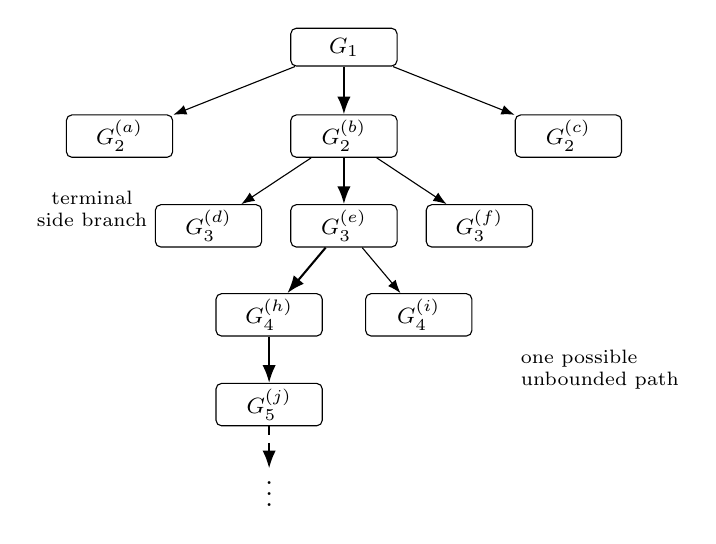
\begin{tikzpicture}[x=1cm,y=1cm,
 gift/.style={draw=black,rounded corners=2pt,fill=white,minimum width=1.35cm,minimum height=.48cm,inner sep=2pt,font=\footnotesize},
 edge/.style={-Latex,thin},main/.style={-Latex,line width=.75pt}]
\node[gift] (g1) at (0,0) {$G_1$};
\node[gift] (a) at (-2.85,-1.13) {$G_2^{(a)}$};
\node[gift] (b) at (0,-1.13) {$G_2^{(b)}$};
\node[gift] (c) at (2.85,-1.13) {$G_2^{(c)}$};
\draw[edge] (g1)--(a); \draw[main] (g1)--(b); \draw[edge] (g1)--(c);
\node[gift] (d) at (-1.72,-2.27) {$G_3^{(d)}$};
\node[gift] (e) at (0,-2.27) {$G_3^{(e)}$};
\node[gift] (f) at (1.72,-2.27) {$G_3^{(f)}$};
\draw[edge] (b)--(d); \draw[main] (b)--(e); \draw[edge] (b)--(f);
\node[gift] (h) at (-.95,-3.4) {$G_4^{(h)}$};
\node[gift] (i) at (0.95,-3.4) {$G_4^{(i)}$};
\draw[main] (e)--(h); \draw[edge] (e)--(i);
\node[gift] (j) at (-.95,-4.54) {$G_5^{(j)}$};
\draw[main] (h)--(j);
\draw[main,dashed] (j)--(-.95,-5.35);
\node at (-.95,-5.57) {$\vdots$};
\node[font=\scriptsize,align=center] at (-3.2,-2.05) {terminal\\side branch};
\node[font=\scriptsize,align=left] at (3.25,-4.1) {one possible\\unbounded path};
\end{tikzpicture}
\caption{\textbf{The Sovereign Gift Tree.} A vertical ``mathematical Christmas tree'' illustrating finitely many admitted next gifts at each node; leaf nodes may terminate while another path continues. Dashes indicate a \emph{possible} infinite continuation, not a proved feature of unrestricted GBG+S. If arbitrarily large depths exist, K\"onig's lemma guarantees at least one infinite path.}
\label{w0:fig:gift-tree}
\end{figure}


\begin{theorem}[Finite-support cumulative consistency]\label{w0:thm:finite}
Let $T_0$ be fixed background axioms and $\Delta_1,\Delta_2,\ldots$ be axiom increments in a fixed finitary proof calculus. Put $\Stage_n=T_0\cup\bigcup_{k=1}^n\Delta_k$ for $n\ge0$ (empty union at $n=0$) and $\Stage_\infty=T_0\cup\bigcup_{k\ge1}\Delta_k$. Then
\[
\Con(\Stage_\infty)\quad\Longleftrightarrow\quad\forall n\ge0\,\Con(\Stage_n).
\]
In particular, $C_n=1$ for all $n\ge0$ implies consistency of the cumulative union.\proofat{w0:pr:finite}
\end{theorem}
\begin{remark}
Theorem~\ref{w0:thm:finite} does \emph{not} assert decidability of $C_n$, consistency of a future unaxiomatized GBG+S theory, equivalence of its changing logics, or the existence of a playable $H_\infty$. It is a theorem about finite proofs in a fixed consequence relation.
\end{remark}

\section{What a gift must promise}\label{sec:typed-braid}
A finite grammar can name gifts without showing that those gifts have
legitimate effects. The construction now needs an interface between an
expression and an activated game. This is the first decisive crossing:
the staged gift theory supplies the accumulating obligations, while typed
models supply a way to satisfy them without silently changing the external
logic. The two descriptions must agree at the same game stage.

The gift grammar and cumulative theory of the preceding sections specify what may be proposed and what mathematical consistency would mean. They do not yet supply a complete contract for implementing a gift. There are two complementary tests: \emph{construct} a model realizing a proposed permission, and \emph{challenge} whether the model and its peers can be combined without silently changing the old rules or the external checker. We begin with an explicit interface.


\begin{definition}[Typed gift contract]\label{w1:def:contract}
A contract for gift $g$ at game stage $G_n$ is a tuple
\[
 \gamma=(g,\iota,\mathsf{Pre},\mathsf{Post},\mathsf{Auth},\mathsf{Obs},\Delta(g),\mathsf{ProofGate}),
\]
where $g$ is a finite atom expression with $|\Supp(g)|=n$; $\iota$ is a state translation or versioned embedding; $\mathsf{Pre}$ and $\mathsf{Post}$ type the transition effect; $\mathsf{Auth}$ declares eligible participants; $\mathsf{Obs}$ specifies an externally fixed capability observation; $\Delta(g)$ is an axiom increment in a fixed metalanguage; and $\mathsf{ProofGate}$ states what evidence an implementation requires. Not all entries are required to be computable for a purely semantic contract. A \emph{certified} admission uses a declared checker for evidence; consistency itself is a mathematical condition, not the checker's verdict.
\end{definition}

The distinction between $\Con(S_n)$ and a computable checker is central. A model of just an operational gadget is not automatically a model of all axioms of the intended theory. Likewise, a certificate accepted by a rewritten verifier is not automatically a sound certificate.



\subsection{The original activation model, now under a typed contract}
The grammar supplies candidate expressions, while the contract identifies what installing one
would actually mean.  We can now return to the foundational permission-registry example
without confusing the dormant construction stage with gameplay.  This return is necessary:
its fixed observation interface makes the later nonredundancy claim precise.

\subsubsection{A transparent toy activation model}
One may interpret a dormant stage by a registry $R_n$ of authorized context-indexed transitions and a mode bit $e=0$ in which no play moves are enabled. To activate, construct $H_n$ in mode $e=1$ with a selector state $q_j$ for each referenced context $j$, and a transition $q_j\to q_j'$ authorized only when its permission lies in $R_n$. Each new permission can expose a previously absent, observable transition. Finite registries yield explicit, finite models; none of this assumes a self-amending external logic.

The comparison is made using a frozen input/output observation interface: for each natural query index $j$, either the activated game returns an authorized success response or it does not. A fresh permission for index $j$ changes that existing interface, rather than merely renaming a state. This toy model validates the \emph{possibility} of successive nonredundant, consistent extensions in a controlled family. It does not model the whole sovereign atom catalogue or prove that checker-rewrite and unrestricted verifier succession can be activated safely.

\begin{proposition}[Infinite consistent gift chain from countably many atoms]\label{w0:prop:infinite}
There is a countably infinite effective atom vocabulary $\Abs=\{a_1,a_2,\ldots\}$ and a locally finite effective composition procedure producing gifts $g_n=a_1\circ\cdots\circ a_n$, one per stage, such that $|\operatorname{supp}(g_n)|=n$, every finite accumulated stage has an explicit model, and $C_n=1$ for all $n$. Under the fixed query interface, each gift changes an observable authorization; this establishes \emph{possibility} of infinite extension, not a mandatory property of GBG+S.\proofat{w0:pr:infinite}
\end{proposition}


\subsection{Finite tagged-permission realizations}
We first isolate a particularly transparent class, without pretending that B1--B23 have all been typed. Let $G$ be a finite, well-formed GBG with a board-player architecture satisfying the original GBG+ rule-completeness and authorization conditions; retain its one designated board-player $P_0$ and its label map $F(r)=\max(0,r-1)$. The game $G$ may have ordinary moves even though the \emph{construction-stage} view is dormant.

\begin{definition}[Finite permission package]\label{w1:def:permission}
Fix a finite list $J=\{j_1,\ldots,j_m\}$ of distinct permission names. For each $j$ introduce two fresh, typed control states $q_j,r_j$ and one candidate rule $\rho_j:q_j\mapsto r_j$, authorized to $P_0$ (or to a specified nonempty role set). A registry $R\subseteq J$ indicates which rules are installed. The activated transition system retains the base game as a designated
subsystem and adds separate permission gadgets. It has explicitly
board-authorized dispatch rules from a designated reachable base state to
each input control state $q_j$, making those contexts reachable without
changing the base subsystem's internal rules. Precisely the $\rho_j$ for
$j\in R$ are installed as success transitions. The dormant display has the same finite state descriptions but all play transitions disabled. Registry updates are external to the dormant game; no undeclared intra-game installation move is posited. In the particular zero-gift realization of the boring game, take $J=\varnothing$ and $R=\varnothing$: no dispatch or success transition is present. A nonempty prospective context list $J$ is part of a separately specified activated package and is not silently added to $H_1$.
\end{definition}

An explicit observable test is $O_R(j)=1$ if and only if the rule $q_j\mapsto r_j$ is authorized in the activated registry. The query meaning, including the name $j$, is frozen before comparing stages; hence installing $j$ changes an existing test rather than merely relabeling a vertex. The finite package size depends on $m$, not on a supposed global infinite permission universe.

\begin{theorem}[Finite tagged-permission realization]\label{w1:th:finite}
For every finite base GBG+ presentation as above, every finite list $J$ and every $R\subseteq J$, there is a finite rule-complete GBG+ presentation of the corresponding activated permission package, with unique board-player $P_0$, declared partial unary transitions, nonempty authorized sets, and the unchanged label map. Every installed permission has a distinct observable effect under $O_R$. Moreover, a finite sequence of registry additions has finite models at every step, and the underlying base game is recovered by restricting to the designated base component and forgetting the dispatch and permission rules.
\prooflink{w1:pr:finite}
\end{theorem}

\begin{remark}[Exact scope]
The component-recovery map is \emph{not} a theorem about preserving every trace after permission additions. The extra $q_j\mapsto r_j$ paths did not belong to the original base. The theorem also does not permit unrestricted checker rewrite, mass promotion, or the unguarded insertion of contradictory axioms. It is a structural result for a specified typed family, not a formal interpretation of an unspecified GBG+S theory.
\end{remark}

\begin{corollary}[Support-indexed nonredundant finite prefixes]\label{w1:co:support}
Let $\{a_i:i\ge1\}$ be a countable effective atom set, and offer only $g_n=a_1\circ\cdots\circ a_n$ at gift index $n$, interpreting $g_n$ as installation of the fresh permission $n$. Every finite prefix has a finite activated model, a single available next gift, and $|\Supp(g_n)|=n$. Its permission-observation vector strictly changes at each stage.
\prooflink{w1:pr:support}
\end{corollary}

This corollary sharpens the permission-registry example: the support requirement is syntactic and the new ability is tested through an explicitly fixed interface. There is no assertion that $a_1,\dots,a_n$ correspond to the actual B1--B23 boundary entries. A further interpretation would be required.

\subsection{Gluing is a separate obligation}
\begin{definition}[Common-base compatible gifts]\label{w1:def:compatible}
Let $L_0$ be a first-order base signature and $T_0$ a base theory. A finite family of gift increments $\Delta_1,\dots,\Delta_m$ is \emph{fiberwise compatible over a model $M\models T_0$} if each $\Delta_i$ is satisfied by an expansion $M_i$ of the \emph{same} underlying $L_0$-structure $M$ and its new nonlogical symbols belong to pairwise disjoint signatures $D_i$ not used by the other increments. Shared symbols are interpreted exactly as in $M$.
\end{definition}

\begin{theorem}[Common-model gluing]\label{w1:th:glue}
If $\Delta_1,\dots,\Delta_m$ are fiberwise compatible over some $M\models T_0$, then $T_0\cup\bigcup_{i=1}^m\Delta_i$ has a model. The same conclusion holds for countably many increments on pairwise disjoint new signatures if all can be expanded over that same $M$. If every $M\models T_0$ admits these simultaneous expansions, the resulting combined theory is conservative for sentences in the base language $L_0$, assuming soundness and completeness of the chosen first-order calculus.
\prooflink{w1:pr:glue}
\end{theorem}

The theorem identifies a mathematically checkable way of combining safe gifts; the sufficient hypothesis is common-model expansion, not simply separate consistency. Its disjointness requirement is a \emph{sufficient guard}, not a claim that interacting gifts cannot ever be combined.

\begin{proposition}[Two individually satisfiable gifts can conflict]\label{w1:prop:conflict}
There exist consistent $T_0$, $T_0\cup\Delta_1$, and $T_0\cup\Delta_2$ such that $T_0\cup\Delta_1\cup\Delta_2$ is inconsistent. This remains true when both increments are individually finite-model satisfiable.
\prooflink{w1:pr:conflict}
\end{proposition}

This is the elementary logical reason to filter \emph{composite} gifts, not just single atoms. In the B4/B5 terminology of the atom catalogue, the independent branches $T+\varphi$ and $T+\neg\varphi$ may each be coherent while their untagged merger is not. A finite graph representing an attempted merge is not itself an inconsistent logic; inconsistency arises if contradictory sentences are unconditionally asserted in one classical theory.


\subsection{Which kind of extension have we actually built?}\label{sec:model-strength}
The same finite permission package can satisfy several different claims of
increasing or incomparable strength. Before inductively composing the
packages, it helps to distinguish what has actually been preserved.

The distinction is quantitative as well as logical: providing a finite
model at each stage does not supply a common size bound for the sequence.
The finite-limit question will return in Section~\ref{sec:limit-braid}.

Work in classical first-order logic with nonempty domains and a fixed cumulative language $L_\infty$. Let $L_0\subseteq L_\infty$ be the base signature, $T_0$ its baseline axioms, and $\Delta_1,\Delta_2,\dots$ properly versioned increments. For successive, versioned gift increments, put
\[
 S_n=T_0\cup\bigcup_{i=1}^n\Delta_i,\qquad S_\infty=T_0\cup\bigcup_{i\ge1}\Delta_i.
\]
Every claim about adding a gift is conditional on the coherence of the typing, the unchanged external consequence calculus, and the correctness of any declared observation interface.

\begin{definition}[Six extension assertions]\label{w2:def:levels}
For a successor theory $S'\supseteq T_0$ and for the full cumulative theory $S_\infty$, consider:
\begin{enumerate}[label=\textup{(\roman*)}]
\item $E$: some model of $T_0$ extends to a model of $S'$;
\item $U$: every model of $T_0$ expands on its existing $L_0$ domain to a model of $S'$;
\item $K$: $S'$ is conservative over $T_0$ for all $L_0$-sentences;
\item $F$: every $S_n$ has some finite model;
\item $L$: $S_\infty$ has a model (possibly infinite);
\item $L_f$: $S_\infty$ has a finite model.
\end{enumerate}
The base reduct in $E,U$ is required to be literally the same $L_0$-structure, not merely to share a title or a set of proof strings.
\end{definition}

For ordinary first-order logic, $U\Rightarrow K$ under completeness, whereas an implication from $K$ back to $U$ is not established by the arguments here and should not be assumed without proof. Also $L_f\Rightarrow F\Rightarrow L$ when all $S_n$ are nested, where the second arrow uses compactness. The reverse of $L\Rightarrow L_f$ is false. We make the more informative separations explicit.

\begin{proposition}[Existence need not lift a chosen base model]\label{w2:prop:lift}
There are a consistent $T_0$ and a consistent successor $S'$ satisfying $E$ but not $U$. Thus finding one consistent successor model does not establish an extension construction valid for all predecessor models.
\prooflink{w2:pr:lift}
\end{proposition}

This is why the structural identity $U\circ E=\mathrm{id}$ cannot simply be reused without verifying that an added gift respects every predecessor presentation. It is also why the weaker goal $\Con(T_0)\Rightarrow\Con(S')$ must be stated with its precise logical strength.

\begin{theorem}[Conservative permissions may be operationally strict]\label{w2:th:independent}
There exists a theory $T_0$ of a nonempty old-language structure and an expansion $S'$ that satisfies $U$ and $K$, but changes a fixed activated-game permission observation from false to true. There also exists a consistent old-language strengthening with no change in that permission observation. Consequently strict operational capability and strict old-language deductive extension are logically independent predicates without an additional bridge axiom.
\prooflink{w2:pr:independent}
\end{theorem}

This explains an apparent paradox in the gift framework: a model can add an executable transition or a new authorization while proving no new sentences of the underlying old-language theory. The converse is equally possible when a theory is strengthened only by a fact about the old domain. A formal benefit measurement must specify which invariant it is tracking. Neither mere syntactic novelty nor a smaller proof horizon is forced by an authorized move.


The stronger all-model expansion property supplies a possible inductive
invariant: if each admitted step expands \emph{every} predecessor model, a
whole finite chain of expansions exists. We now formulate the exact
cumulative-consistency test for that chain, allowing interaction axioms to
appear at any stage.

\subsection{Cumulative admission and the missing uniformity}
Two questions have now met. The gift grammar measures progress along an
admitted history; the common-model construction measures compatibility
between previously separate permissions. Neither answers the other.
A consistency proof for the complete gift must pass from \emph{local models}
to the \emph{entire accumulated axiom set}.  The natural bridge is induction over \emph{cumulative}
contracts, rather than over the bare names of atoms.  This formulation records the
November 19 AMLD+0 continuation as a manuscript-level derivation; it is not an
independently verified BANK deposit~\cite{amldledger}.

\begin{theorem}[Inductive Composite Gift Preservation]\label{br:th:inductive}
Let $T_0$ be a consistent theory in a fixed classical finitary proof calculus, and
let $T_k=T_{k-1}\cup\Delta_k$ for $1\le k\le n$. Assume the fixed
calculus has the usual finite-conjunction and deduction principles of
classical first-order logic (and soundness and completeness when passing to
models). Each $\Delta_k$ must include
\emph{every} interaction axiom activated at that prefix, not merely the axioms
of its newest atomic gift.  Then the following conditions are equivalent:
\begin{enumerate}[label=\textup{(\roman*)}]
\item $\Con(T_n)$;
\item $\Con(T_k)$ for every $0\le k\le n$;
\item for every $1\le k\le n$ and every finite $F\subseteq\Delta_k$,
$T_{k-1}\not\vdash\neg\bigwedge F$, where an empty conjunction denotes $\top$.
\end{enumerate}
For ordinary first-order logic these are also equivalent to the existence of a
model for every $T_k$. Thus a sound cumulative admission step at each stage
preserves consistency for the entire finite composite.
\prooflink{br:pr:inductive}
\end{theorem}

The theorem is a sharp characterization of \emph{what must be checked}, not a
uniform algorithm for performing those checks. It also does not imply that
consistency of $T_0+\Delta(a)$ for every isolated atom $a$ guarantees
consistency of their joint extension: the interaction axioms in $\Delta_k$
may be decisive.  A separately consistent alternative branch is not
silently merged into the current theory.  In particular, the B5
unguarded union of $\varphi$ and $\neg\varphi$ is a negative boundary,
not a gift that must be admitted.

\begin{corollary}[Consistency of a cumulative chain]\label{br:co:chain}
If $\Con(T_0)$ and every actual installation step satisfies
$\Con(T_{k-1})\Rightarrow\Con(T_k)$, then $\Con(T_n)$.
For an increasing countable sequence with the same finitary consequence
relation, consistency of all finite stages also entails consistency of
the union $\bigcup_{k\ge0}T_k$.
\prooflink{br:pr:chain}
\end{corollary}

This extends the finite-support consistency principle in
Theorem~\ref{w0:thm:finite}: every quantified increment must include
its newly activated cross-gift obligations.  The result will matter again when
we ask whether infinitely many consistent stages form a usable limit.

\subsection{The proof-induction alternative}
There is a complementary, potentially shorter route.  In the formal-system
vocabulary $F=(x,y,z)$, formulas lie in $y$ and finite proofs are successive
applications of rules in $z$. Tenneson's \emph{Depths of a Simulation and
Formalized Self-Awareness}, ATLAS v2 corrected edition, gives the exact
formula-sequence framework in Definitions~1.2--1.5 and an induction principle
on proof lines in Theorem~1.10~\cite{depthsv2}.  Structural induction on a
recursively defined formula grammar and induction on derivation lines are
different arguments.  The former can define an interpretation; the latter
can transport proofs.

\begin{proposition}[Interpretation criterion for relative consistency]\label{br:prop:interpret}
Let $T_S$ and $T_+$ be fixed formal theories with distinguished
contradictions $\bot_S$ and $\bot_+$. Suppose a total translation $\tau$
on source formulas maps every axiom of $T_S$ to a theorem of $T_+$,
maps each application of a source inference rule to a valid finite
target derivation, and satisfies $\tau(\bot_S)=\bot_+$.
Then $\Con(T_+)\Rightarrow\Con(T_S)$.
\prooflink{br:pr:interpret}
\end{proposition}

This statement does \emph{not} supply the translation for the entire sovereign
atom grammar.  It clarifies the transfer obligation: a claimed interpretation
must respect every admitted axiom and rule, including versioned verifier
updates.  No ability to express a formula is itself a proof of its consistency.

\subsection{Operational stopping versus maximality}
A termination command and a proof of maximality are different mathematical statements. Write $\Adm(G_n,g)$ for semantic admissibility and
\[
 \mathsf{Max}(G_n)\;:\Longleftrightarrow\;\neg\exists g\,\Adm(G_n,g).
\]
Our stopping protocol can stop after a chosen inconsistent proposal; that event does not assert $\mathsf{Max}(G_n)$. We make the separation explicit.

\begin{proposition}[Stopped need not mean maximal]\label{w1:prop:stop}
There exists a finite gift-choice system with a consistent initial stage, two proposed next gifts $u,v$, and a policy that stops on the rejected candidate $u$, although $v$ is admissible and nonredundant. Consequently, $\mathsf{Stop}(G_n)$ does not entail $\mathsf{Max}(G_n)$ without an additional exhaustive-completeness condition.
\prooflink{w1:pr:stop}
\end{proposition}

Likewise local finiteness of the set of \emph{actual} admissible children does not imply a finite computable candidate search: a finite set may have its sole member at arbitrarily high code index. The single-optional-gift halting construction in Theorem~\ref{w0:thm:next} will demonstrate this. Nor does a numerical bound on distinct atom supply give an algorithm for determining whether the current next-gift set is empty. It limits the number of accepted steps.


The induction theorem settles preservation \emph{along} an admitted path,
while Theorem~\ref{w1:th:glue} says when separately modeled permissions can
be placed in one structure. Neither proves that a next gift exists, or that
no admissible gift remains. Even when the acceptance rule is exact, can
anyone determine when the last acceptable gift has arrived?


\section{From isolated gifts to an inductive research program}\label{br:sec:handoff}
The typed-contract discussion above provides the first side of a bridge. The next strands investigate three distinct questions: can overlapping finite constraints be solved jointly, can a restricted MOBILITY model actually receive GRANT, and can such constructions be iterated without relying on atom names? None of these questions may be replaced by the assertion that an unverified candidate is simply ``safe.'' The explicit compatibility witness comes first because the preservation induction otherwise risks hiding the main difficulty in its inductive hypothesis.

\paragraph{Two atom namespaces.} The historical catalogue above uses \emph{H:B1} for Verifier Succession, \emph{H:B11} for Cross-System Trade, and \emph{H:B14} for Clock Rewrite. The November 21 induction experiment uses \emph{N:B1=MOBILITY}, \emph{N:B2=GRANT}, and reindexes the remaining candidates locally. Historical B-numbers in the six shortcut constructions below refer to \emph{H:B-numbers}. This is a research bookkeeping convention, not an axiom change. The old non-sovereignty restriction, sovereign identity, cumulative gate, and exactly-$n$-distinct-atom grammar remain unchanged.


\section{Acyclic compatibility: the finite join-tree construction}\label{br:sec:compat}
\noindent\textit{Integrated from the original Acyclic compatibility: the finite join-tree construction research note, November 20, 2026. The exact source filename and bytes are retained in the accompanying preservation archive.}

\begin{quote}\small\textbf{Source abstract (preserved).} We prove a finite-constraint compatibility theorem that can be applied to explicitly specified sovereign-gift contracts with overlapping authorization, verification, and history variables. If the contract scopes admit a join tree, upward filtering followed by downward reconstruction decides joint satisfiability and constructs a witness. The theorem is a specialization of the standard acyclic constraint-satisfaction principle, not a claim of a new general theorem in database or constraint theory. Its application to GBG+S is conditional on a faithful finite formalization of all relevant gift requirements. It gives a rigorous restricted route toward the fourth outstanding compatibility obligation, but does \emph{not} establish \(\Con(\mathrm{GBG+})\Rightarrow\Con(\mathrm{GBG+S})\).\end{quote}





\subsection{Research context and scope}
The sovereign-gift program distinguishes a typed candidate atom from an admitted composite gift. In the source manuscript, the gift at index \(n\) is a finite expression over an atom supply \(A\) with exactly \(n\) distinct atoms in its support. Admission requires, among other things, well-defined legal effects, nonredundancy, and cumulative consistency in a fixed external logic. External gift installation is distinct from the internal moves of an activated game. A finite model of a permission gadget is not automatically a model of the entire intended GBG+S theory.

Four obstacles were identified for the full relative-consistency target: fixing the complete sovereign theory, completing provisional atom contracts, constructing an interpretation of that full theory, and explaining how authorization, verification, and historical commitments interact in composite gifts. The present theorem addresses the \emph{fourth} obstacle on a restricted, explicitly finite class. It is not a replacement for the first three.

\subsection{Finite typed constraint representation}
\begin{definition}[Finite gift-constraint instance]
A \emph{finite typed gift-constraint instance} comprises a finite variable set \(X\); for every \(x\in X\), a finite nonempty domain \(D_x\); and a finite indexed family \((S_i,R_i)_{i\in I}\) with \(S_i\subseteq X\) and explicitly given relation
\[
R_i\subseteq\prod_{x\in S_i}D_x.
\]
A global assignment \(t\in\prod_{x\in X}D_x\) is a \emph{realization} if \(t|_{S_i}\in R_i\) for every \(i\in I\). Relations may overlap, and each relevant governing or cross-gift interaction must be included as a constraint.
\end{definition}

The vacuous instance with no constraint scopes is satisfiable because each of
the finitely many domains is nonempty. In the join-tree construction below,
we therefore assume at least one constraint scope; this avoids a fictitious
root for an empty tree.

\begin{definition}[Join tree]
A \emph{join tree} for the constraint family is a tree with vertex set \(I\) such that, for each variable \(x\in X\), the set \(\{i\in I:x\in S_i\}\), when nonempty, induces a connected subtree. This is the running-intersection condition. Variables occurring in no scope may be assigned arbitrarily from their nonempty domains.
\end{definition}

\begin{theorem}[Acyclic sovereign-gift compatibility]\label{compat:thm:main}
Given a finite typed gift-constraint instance whose scopes admit a join tree, there is a terminating procedure that decides whether the entire instance has a realization and constructs one exactly when one exists. Overlap among contract scopes is permitted. If the constraints faithfully encode \emph{all} axioms and operational requirements of a particular finite GBG+S fragment, any produced realization yields a model of that fragment, and therefore establishes consistency of that fragment relative to a sound proof calculus.
\end{theorem}

\phantomsection\label{br:compat:stmt:1}\prooflink{br:compat:proof:1}


\begin{remark}[What the theorem does not assume]
Acyclicity concerns the \emph{scopes of constraints}, not a claim that source gift atoms are independent or that their effects commute. The theorem neither decides arbitrary semantic consistency predicates nor turns a Boolean flag asserting ``verified'' into an actual sound verifier receipt. Those requirements must be represented and justified externally.
\end{remark}

\subsection{A shared-resource finite example}
Let \(a,v,h,m\in\{0,1\}\) denote, respectively, a specified authorization, modeled acceptance of verification evidence, preservation of a specified history record, and execution of a specified move. Consider
\[
R_1(a,v): a\Rightarrow v,\qquad
R_2(v,h): v\Leftrightarrow h,\qquad
R_3(h,m):m\Rightarrow h.
\]
The scopes \(\{a,v\},\{v,h\},\{h,m\}\) form a path and hence a join tree. The assignment
\( (a,v,h,m)=(1,1,1,1) \) realizes the conjunction. There are exactly five satisfying assignments: one with \(v=h=0\), necessarily \(a=m=0\), and four with \(v=h=1\) and arbitrary \(a,m\). This is an illustrative finite constraint model, not evidence that an actual external verifier or gameplay process executed.

\subsection{Why local compatibility is not enough}
\begin{proposition}[A cyclic obstruction]
There exist three binary-variable constraints each individually satisfiable, with any two jointly satisfiable, but with no common realization.
\end{proposition}
\phantomsection\label{br:compat:stmt:2}\prooflink{br:compat:proof:2}


\begin{remark}
Finite cyclic constraint systems are still decidable by exhaustive enumeration. What fails is the unrestricted inference from pairwise compatibility to global compatibility, and the special join-tree local-to-global method.
\end{remark}

\subsection{Application discipline and original target}
Before applying Theorem~\ref{compat:thm:main} to any of the twelve retained sovereign atom candidates, a separate construction must justify the following.
\begin{enumerate}[label=(\arabic*),leftmargin=*]
\item All relevant variables and typed contract relations are explicitly defined, including any global and cross-gift interactions.
\item Shared authorization and unique sovereign identity are respected.
\item Verification predicates stand for the correct declared evidence and its genuine soundness obligations, not merely unchecked acceptance flags.
\item Historical commitments preserve their required version and ordering semantics.
\item Gift support, cumulative consistency, admission/STOP rules, and the distinction between external installation and internal gameplay remain correctly represented.
\item Satisfying assignments correspond to models of the claimed \emph{entire finite fragment}, rather than to a simplified operational gadget.
\end{enumerate}

When these conditions hold, the theorem supplies a constructive method for the fragment's compatibility obligation. It does not supply those conditions for all actual atoms. In particular, the relative-consistency statement
\[
\Con(\mathrm{GBG+})\Longrightarrow\Con(\mathrm{GBG+S})
\]
remains unproved. A universally faithful reduction of the intended GBG+S theory to this finite framework has not been constructed.

\subsection{Proof status and next obligation}
\noindent\textbf{Established here:} the exact acyclic finite-constraint theorem, a witness-construction proof, and a finite cyclic obstruction. These are standard constraint-theoretic mathematical principles applied as a conditional framework for the fourth sovereign-gift compatibility block.

\medskip\noindent\textbf{Open:} faithful complete contracts for actual atoms, an exact axiomatization of unrestricted GBG+S, uniform compatibility treatment for all relevant interactions, and the desired relative consistency theorem.

\medskip\noindent\textbf{Verification status:} mathematical manuscript proof; no proof-kernel or independent external verifier receipt. This result must not be labeled a certified AMLD+0 BANK theorem until checked under the frozen proof policy.

\vspace{1.3em}\noindent\textbf{Research sources.} The internal source framework is \emph{From the Boring Game to the Last Gift}, especially Sections 3, 6, and 7 (gift grammar, cumulative admission, typed contracts, common-model gluing, and composite gift preservation). The present note is intended for subsequent integration into a longer GBG+S research article, subject to audit.



\section{MOBILITY and GRANT: a restricted uniform construction}\label{br:sec:mobgrant}
\noindent\textit{Integrated from the original MOBILITY and GRANT: a restricted uniform construction research note, November 21, 2026. The exact source filename and bytes are retained in the accompanying preservation archive.}

\begin{quote}\small\textbf{Source abstract (preserved).} We give an explicit, uniform construction extending every \emph{GRANT-ready} GBG+-style MOBILITY transition model by a nontrivial sovereign GRANT capability. The construction preserves each original state, each original labeled partial transition (including undefinedness), and each original authorization, while adding fresh, versioned states and two new authorized transition labels. It retains one sovereign identity and a prescribed two-board $E/S$ reporting invariant. We prove a corresponding relative-consistency result only for a formal theory whose models satisfy the stated extension interface and whose added axioms precisely specify this construction. This does \emph{not} establish consistency of unrestricted GBG+S, nor prove that the as-yet provisional GRANT atom is fully axiomatized. An adversarial audit identifies the hypotheses on which the argument depends.\end{quote}





\subsection{Question and scope}
Let $M$ denote the candidate MOBILITY atom and $G$ the candidate GRANT atom. The desired transfer is
\begin{equation}\label{mobgrant:eq:target}
\Con(T+M)\;\Longrightarrow\;\Con(T+M+G).
\end{equation}
As written, \eqref{mobgrant:eq:target} need not hold: independently interpretable extra axioms can conflict with existing ones. The question is whether there is a \emph{uniform expansion construction} for a natural class of MOBILITY models that realizes an actual, observable GRANT without changing original legal behavior. The singleton bijection $\{(M,G)\}$ plays no role in the consistency proof.

The construction below is at the level of activated transition presentations, not self-amendment of a deductive calculus. It honors the distinction between external acquisition of gifts and legal actions in the activated game. It is intentionally narrower than the full sovereign theory.

\subsection{A GRANT-ready MOBILITY model}
Fix an activated, rule-complete transition presentation
\[
H_M=(Q,A,\{\delta_a\}_{a\in A},\Auth,\mathcal P,S,P,\Hist,\operatorname{rep}_2,\pi),
\]
where $Q$ is a set of complete, versioned game states; every $\delta_a:Q\rightharpoonup Q$ is a declared partial unary rule; $\Auth(q,a)$ specifies the authorized actor; $\mathcal P$ contains one distinguished sovereign $S$ and an ordinary player $P\ne S$; $\Hist(q)$ records the relevant prior events; $\operatorname{rep}_2$ gives the alternative-board report in $\{E,S\}$; and $\pi$ denotes any required projection to the designated base game. The identity of $S$ is invariant across legal transitions.

\textbf{Definition (GRANT-ready).} The presentation $H_M$ is GRANT-ready for a named action $\rho$ if:
\begin{enumerate}
\item There is a reachable state $q\in Q$ after a lawful MOBILITY event, where $S$ occupies board 2. Every original report $S$ on board 2 implies a relevant earlier MOBILITY event in the recorded history; the event was unavailable under the native board's earlier rule set but is lawful in the MOBILITY extension.
\item At $q$, $\rho$ is a meaningful, well-typed candidate action for $P$ and $P$ is \emph{not} authorized to perform it. There is a well-formed hypothetical successor configuration after $P$ performs $\rho$.
\item The state coding and rule presentation admit two fresh versioned states, two fresh labels, and extensions of the history and report functions. The new labels are not subject to a legacy totality or exclusivity rule. Existing $\delta_a$ are not rewritten.
\item Any obligatory base-game projection $\pi$ and other preserved structural invariants permit the new transitions, for example by mapping a permission-only transition to a designated stutter in the base presentation. No existing axiom universally forbids new authorized transitions in a new activated version.
\item The fixed observation interface can query whether $P$ is authorized for $\rho$ in a specified state. Its meaning is not redefined after extension.
\end{enumerate}
These are independently checkable structural and interface assumptions, not the assertion that the desired extension is already consistent. In particular, item 4 is a substantive contract obligation.

\subsection{Uniform construction}
Choose the witness $(q,P,\rho)$ from the GRANT-ready structure. Add two fresh, distinct states $q_g,q_u\notin Q$:
\[
Q'=Q\sqcup\{q_g,q_u\}.
\]
The physical coordinates and sovereign identity of $q_g$ agree with those of $q$. The state $q_g$ records a new permission $\mathrm{Permit}(P,\rho)$; $q_u$ records the result of executing $\rho$ from $q_g$. Set
\[
\Hist(q_g)=\Hist(q)\mathbin{\raisebox{0.15ex}{$\smallfrown$}}[\mathrm{grant}],\qquad
\Hist(q_u)=\Hist(q)\mathbin{\raisebox{0.15ex}{$\smallfrown$}}[\mathrm{grant},\rho].
\]
For $x\in\{q_g,q_u\}$, use the original $q$'s board-2 sovereign location and reporting value, so the earlier lawful MOBILITY event witnesses any report of $S$.

Let $\gamma$ be a fresh sovereign-GRANT label and $\widehat\rho$ a fresh authorized-recipient label. Define
\begin{align*}
\delta'_a(s)&=\delta_a(s) &&(a\in A,\ s\in Q),\\
\delta'_a(x)&\text{ undefined} &&(a\in A,\ x\in\{q_g,q_u\}),\\
\delta'_{\gamma}(q)&=q_g,\\
\delta'_{\widehat\rho}(q_g)&=q_u,
\end{align*}
with $\delta'_{\gamma}$ and $\delta'_{\widehat\rho}$ undefined elsewhere. The new authorization assignments are $\Auth'(q,\gamma)=S$ and $\Auth'(q_g,\widehat\rho)=P$. All old authorization assignments on original state/action pairs remain unchanged. All other new actions are absent.

The old system embeds by the literal inclusion $i:Q\hookrightarrow Q'$. Its labeled graph is precisely the restriction of the enlarged labeled graph to original labels and original states. It is \emph{not} claimed that original states have exactly the same total menu of labels, because $q$ now also enables $\gamma$.

\begin{theorem}[Uniform GRANT extension]\label{mobgrant:thm:main}
Every GRANT-ready MOBILITY presentation $H_M$ has an extended presentation $H_{MG}$ with the following properties:
\begin{enumerate}
\item The original states, original action-label transitions (including non-applicability), and original authorizations are preserved exactly.
\item The extension has exactly one sovereign identity $S$, preserves the two-board $E/S$ reporting implication, and records its new events by append-only history.
\item All new transitions are declared partial unary rules with named authorized actors and unique successors; all required projections and structural invariants continue to hold under the GRANT-ready interface requirements.
\item GRANT has a distinct observable effect: from a reachable state, $S$ can issue $\gamma$ and $P$ can subsequently execute $\widehat\rho$, although $P$ could not execute $\rho$ at $q$ in the original model.
\end{enumerate}
If $Q$ is finite, the construction increases its cardinality by exactly two. If $Q$ is infinite, the construction is still a finite extension of the rule presentation.
\end{theorem}
\phantomsection\label{br:mobgrant:stmt:1}\prooflink{br:mobgrant:proof:1}


\subsection{The logical transfer that does, and does not, follow}
The theorem concerns a structural category of typed activated game presentations. A model of an arbitrary original theory may have global first-order restrictions invalidated by the new states, so $Q\subseteq Q'$ alone is \emph{not} a first-order model expansion preserving every old sentence.

\begin{proposition}[Conditional relative consistency]\label{mobgrant:prop:relative}
Let $T_M^{\mathrm{ready}}$ be a first-order theory whose models are GRANT-ready presentations under a fixed, explicitly sorted encoding. Let $T_{MG}^{\mathrm{ready}}$ be a target theory with an untouched original-game sort and an additional extended-game sort, together with symbols for the embedding, new states, transitions, observations, histories and projections. Assume the target axioms are exactly those satisfied by the construction of Theorem~\ref{mobgrant:thm:main}, including all shared-interface requirements and interaction axioms. Then
\[
\Con(T_M^{\mathrm{ready}})\Longrightarrow\Con(T_{MG}^{\mathrm{ready}}).
\]
Indeed, every model of $T_M^{\mathrm{ready}}$ has an expansion in the extended sorted language satisfying $T_{MG}^{\mathrm{ready}}$.
\end{proposition}
\phantomsection\label{br:mobgrant:stmt:2}\prooflink{br:mobgrant:proof:2}


\begin{remark}[What remains unproved]
The unrestricted implication\[\Con(\mathrm{GBG+S}+M)\Rightarrow\Con(\mathrm{GBG+S}+M+G)\]remains open because a complete, independent specification of the intended GRANT atom, full cumulative gift contracts, and their global interaction axioms has not been supplied. In particular, the proposition does not assume that arbitrary GBG+S models are GRANT-ready.
\end{remark}

\subsection{Adversarial audit and source-faithfulness}
\begin{enumerate}
\item \textbf{No new-action prohibition.} A base axiom asserting that no extension may ever authorize $\rho$ blocks the construction. Such a model is not GRANT-ready; omitting this boundary would make the claim false.
\item \textbf{No-recipient obstruction.} A game without a suitable ordinary player or well-typed candidate action cannot realize this particular nontrivial grant.
\item \textbf{Strong preservation ambiguity.} Original actions and successors are preserved exactly, but the set of all actions available at original $q$ grows. Requiring an unchanged total action menu at every original state would contradict the chosen attachment method.
\item \textbf{Historical and board-report obligations.} The two new states inherit a lawful prior MOBILITY event; $S$ denotes one identity, not a second sovereign. A report of $S$ is not used to retroactively legalize an impossible event.
\item \textbf{Gift grammar.} The staged sequence may be represented by first gift $g_1=M$ and second composite gift $g_2=K(M,G)$, with $|\supp(g_1)|=1$ and $|\supp(g_2)|=2$. The gift-installation steps are external, whereas $\gamma$ and $\widehat\rho$ are activated-game moves. This does not automatically establish every admission-gate or checker obligation for unrestricted GBG+S.
\item \textbf{Generality to other atoms.} The proof uses GRANT specifically to obtain a fresh permission followed by an executable action; its graph-extension mechanism is more general. This note does not assert that arbitrary other atoms preserve axioms controlling verification, clocks, abdication or cumulative sovereignty.
\end{enumerate}

\subsection{Settlement record}
\textbf{P (proved conditionally):} Theorem~\ref{mobgrant:thm:main} and Proposition~\ref{mobgrant:prop:relative} for the explicitly defined subclass and sorted encoding.\par
\textbf{R (boundary):} Invertibility of a singleton atom-name map and separate consistency of candidate atoms do not establish their joint consistency.\par
\textbf{D (dependency):} Full transfer requires a faithful GRANT operational contract and checks against all global GBG+S axioms, projections, verification gates and activated interactions.\par
\textbf{U (unresolved):} The unrestricted GBG+S relative-consistency target remains open. No independent formal verifier receipt is claimed.

\small\emph{Source basis:} the reviewed \emph{From the Boring Game to the Last Gift}, Sections 2--3 and 6--7. This restricted result is not a certified proof of full GBG+S consistency.



\section{The indexed-preservation route: uniformity and induction}\label{br:sec:induct}
\noindent\textit{Integrated from the original The indexed-preservation route: uniformity and induction research note, November 21, 2026. The exact source filename and bytes are retained in the accompanying preservation archive.}

\begin{quote}\small\textbf{Source abstract (preserved).} We investigate two related conjectures: (a) whether consistency-preserving extension can be characterized without reference to the name of an operation, and (b) whether an indexed family of sovereign gifts, beginning with MOBILITY and GRANT, can be proved cumulatively consistent relative to GBG+ by induction. We restate and prove exact semantic and finite-obstruction criteria for a specified first-order extension; give a concrete class of definitional extensions; prove a stronger, compositional model-expansion theorem suitable for induction; and show that compatible extension witnesses yield consistency of every finite prefix, and, by compactness, their union. We also give a sharp counterexample: separately consistent atoms may have an inconsistent union. The retained sovereign atoms have not all been shown to satisfy the extension hypotheses. These are general metatheorems and conditional research tools, not a settlement of unrestricted GBG+S relative consistency; no novelty over established model-theoretic principles is claimed.\end{quote}


\vspace{0.3em}
\begin{tcolorbox}[colback=gray!6,colframe=gray!45,boxrule=0.4pt,arc=1mm]
\small\textbf{Status.} The identity-independent logical criterion and the conditional indexed-preservation theorem below are elementary classical first-order metatheorems. The revised note adds an explicit definitional-extension test and distinguishes literal expansions from changes to existing game-state domains. Their application to the actual retained sovereign atoms is \emph{unresolved}. In particular, this note does \emph{not} prove \(\Con(\Gb)\Rightarrow\Con(\GG)\), nor does it claim independent machine verification.
\end{tcolorbox}




\subsection{Pass I: formalization and revised indexing}

Fix a classical finitary first-order metalogic. Let \(T_0\) be an \emph{explicitly fixed} first-order axiomatization of \(\Gb\), with language \(L_0\). For successive atoms \(B_i\), let \(\Delta_i\) be their independently declared axiom sets and let \(L_i\supseteq L_{i-1}\) be the cumulative languages. Write
\begin{equation}\label{induct:eq:prefix}
T_n := T_0\cup\bigcup_{i=1}^{n}\Delta_i, \qquad
\mathsf{Target}(n):\quad \Con(T_0)\Longrightarrow\Con(T_n).
\end{equation}
The extension must not quietly reinterpret a pre-existing symbol. In the theorems below, a \emph{literal expansion} in a nested many-sorted language leaves the domains of every \emph{old} sort, and every old symbol interpretation, unchanged. Consequently, it cannot add elements to an existing game-state sort. A GRANT-like construction adding states must instead place its versioned state space in a \emph{new} sort while retaining the original sort, or use an explicitly defined interpretation/embedding theorem that does not claim literal reduct equality. This restriction is mathematically substantive: universal sentences of the base theory may cease to hold if its old domain is enlarged. Changes to game rules, permissions or verification must be represented by explicit versions, sorts, maps or transition relations, rather than by changing the external consequence relation.

\subsubsection{Working index, not a change to historical names}

In this note \(B_1:=\mathrm{MOBILITY}\) and \(B_2:=\mathrm{GRANT}\). The remaining ten retained candidates are reindexed \emph{locally} as follows. The old B-names are retained in the second column for historical cross-reference; the new numbers do not assert any dependence theorem.
\begin{center}
\small
\begin{tabular}{@{}>{\bfseries}l l p{3.55in}@{}}
\toprule
New & Historical & Candidate \\
\midrule
\(B_1\) & M & MOBILITY (provisional) \\
\(B_2\) & G & GRANT (provisional) \\
\(B_3\) & old B1 & Verifier Succession (undecided) \\
\(B_4\) & old B2 & Unlock--Revise--Relock \\
\(B_5\) & old B4 & Fork \\
\(B_6\) & old B8 & Abdicate (guarded) \\
\(B_7\) & old B9 & Resurrect (guarded) \\
\(B_8\) & old B11 & Cross-System Trade \\
\(B_9\) & old B14 & Clock Rewrite \\
\(B_{10}\) & old B18 & Copy--Promote \\
\(B_{11}\) & old B19 & One Office, Many Executors \\
\(B_{12}\) & old B20 & Finite-Step Replication \\
\bottomrule
\end{tabular}
\end{center}
These are \emph{candidate} operations. Their inclusion in a catalogue is not proof of well-definedness, realizability or consistency.

The earlier GBG+S gift grammar also imposes a separate requirement: gift number \(n\) has exactly \(n\) distinct atomic ingredients in its support. One may \emph{propose} a composite \(K(B_1,\dots,B_n)\) of support size \(n\), but an indexed list by itself does not prove that the actual grammar \(K\) can form it or that the resulting gift is admissible. The present theorem addresses the logical consistency of cumulative \emph{prefix theories}; faithful implementation of the stage protocol is an additional obligation.

\subsection{Pass II: general preservation theorems}
\subsubsection{An exact operation-independent criterion}

\begin{theorem}[Exact consistency criterion]\label{induct:thm:exact}
Let \(T\) be any classical first-order theory in language \(L\), and let \(\Delta\) be any set of sentences in an extended language \(L'\supseteq L\), with \(T\) interpreted using its original symbols. Then the following are equivalent:
\begin{enumerate}[label=(\roman*)]
\item \(T\cup\Delta\) is syntactically consistent;
\item for every finite \(F\subseteq\Delta\), \(T\not\vdash\neg\bigwedge F\), where \(\bigwedge\varnothing:=\top\);
\item there exists \(\mathcal N\models T\cup\Delta\);
\item there exist \(\mathcal M\models T\) and an expansion \(\mathcal N\models T\cup\Delta\) whose \(L\)-reduct is \(\mathcal M\).
\end{enumerate}
The criterion is independent of the particular name or subject matter of the proposed operation, but it restates satisfiability rather than providing a generally effective or syntactically local certification method. We do not claim this standard equivalence is a new logic theorem.
\end{theorem}
\phantomsection\label{br:induct:stmt:1}\prooflink{br:induct:proof:1}


This criterion is exact but not generally an effective algorithm. In particular, a search that has found no contradiction is not a proof of consistency. Moreover, mere consistency of an extension is weaker than the ability to expand \emph{every} model of the base.

\begin{definition}[Uniform expansion property]\label{induct:def:uep}
A specified operation with axioms \(\Delta\) has the \emph{uniform expansion property} over \(T\), abbreviated \(\mathsf{UEP}(T,\Delta)\), if
\[
\forall\mathcal M\models T\;\exists\mathcal N\models T\cup\Delta
\quad (\mathcal N\restr L=\mathcal M).
\]
The equality of reducts is literal: old-sorted domains as well as old-symbol interpretations are preserved. The new language may introduce additional sorts; relations on the old sorts can be extended only when they are fresh relation symbols.
\end{definition}

\begin{proposition}[Sufficiency and conservativity]\label{induct:prop:uep}
If \(\mathsf{UEP}(T,\Delta)\), then \(\Con(T)\Rightarrow\Con(T\cup\Delta)\). Furthermore, \(T\cup\Delta\) is conservative over \(T\) for sentences of \(L\). The uniform expansion property is not necessary for mere consistency of \(T\cup\Delta\).
\end{proposition}
\phantomsection\label{br:induct:stmt:2}\prooflink{br:induct:proof:2}


\subsubsection{A noncircular sufficient test: explicit definitions}

\begin{proposition}[Definitional-extension certificate]\label{induct:prop:definitional}
Let $T$ be a first-order theory in $L$. Construct $L'$ in finitely many stages by adding only new relation symbols $R$ with axioms
\[
\forall\bar x\,(R(\bar x)\leftrightarrow\varphi_R(\bar x)),
\]
where $\varphi_R$ uses symbols already available at that stage; and new function symbols $f$ with axioms
\[
\forall\bar x\,\varphi_f(\bar x,f(\bar x)),
\]
where the preceding theory proves $\forall\bar x\,\exists!y\,\varphi_f(\bar x,y)$.
Then every $L$-model of $T$ has an $L'$-expansion satisfying the defining axioms. The resulting theory is consistent relative to $T$ and conservative for $L$-sentences.
\end{proposition}
\phantomsection\label{br:induct:stmt:3}\prooflink{br:induct:proof:3}


\noindent This gives a \emph{proof-checkable form of obligation}: a proposed function needs a supplied derivation of unique existence; the definitions themselves can be inspected. It does not give a terminating general proof-search procedure. It does not prove that arbitrary gift operators are mere definitional extensions or that such operations have the required physical, authorization or strategic effects. A nontrivial fresh \emph{new-sorted} finite transition system can also be adjoined, leaving the base sorts untouched, but this alone is not faithful MOBILITY or GRANT.

\subsubsection{A compositional invariant-preservation theorem}

The exact criterion is largely logical; to implement gifts we seek a stronger constructive contract. Let \(\mathcal K_n\subseteq\Mod(T_n)\) be a class of \emph{eligible} models equipped with any further semantic invariant \(I_n\): fixed sovereign identity, declared and legal transitions, recorded history, permitted object-level changes, base-game projection, admission commitments, and separation of external gift installation from activated moves. The requirements must be specified \emph{independently} of the assertion that a desired extension is consistent. In particular, the set $\mathcal K_n$ is not a newly invented consistency oracle: one must give independently checkable axioms/invariants and a construction that is proved to land in the indicated class.

\begin{theorem}[Uniform indexed model-preservation]\label{induct:thm:indexed}
Assume \(\mathcal K_0=\Mod(T_0)\) and, for each \(i\geq1\), an explicitly specified construction
\[
E_i:\mathcal K_{i-1}\longrightarrow\mathcal K_i
\]
is total on its stated domain, with \(E_i(\mathcal M)\restr L_{i-1}=\mathcal M\). The languages are nested many-sorted languages, so any genuinely new versioned states inhabit new sorts, not the old state sort. Then for every finite \(n\), every model of \(T_0\) has an iterated expansion to a model of \(T_n\). Consequently
\begin{equation}\label{induct:eq:result}
\forall n<\omega,\qquad
\Con(T_0)\Longrightarrow\Con(T_n).
\end{equation}
Each \(T_n\) is also conservative over \(T_0\) for \(L_0\)-sentences.
\end{theorem}
\phantomsection\label{br:induct:stmt:4}\prooflink{br:induct:proof:4}


\begin{remark}[A weaker sufficient variant]
For consistency alone, it suffices that \(\mathcal K_0\) contain \emph{some} model of \(T_0\) whenever \(T_0\) is consistent, and that each \(E_i\) be defined on reachable \(\mathcal K_{i-1}\). The resulting conclusion need not be conservative for every \(T_0\)-model. The all-model version above is intentionally stronger and easier to compose. For either version, a mere declaration that $E_i$ maps eligible models to eligible models is not an operational proof: the particular construction and its preservation lemma must be established separately.
\end{remark}

\begin{corollary}[Infinite cumulative theory]\label{induct:cor:omega}
Under Theorem~\ref{induct:thm:indexed}, \(\Con(T_0)\Rightarrow\Con(T_\omega)\), where \(T_\omega=\bigcup_{n<\omega}T_n\). The union is also conservative over $T_0$ for old-language sentences.
\end{corollary}
\phantomsection\label{br:induct:stmt:5}\prooflink{br:induct:proof:5}


\subsection{Pass III: counterexamples and failure modes}

\begin{counterexample}[Separate safety does not imply cumulative safety]\label{induct:cx:pn}
Assume \(T_2\) is consistent and \(p\) is a fresh nullary predicate. Let \(\Delta_3=\{p\}\) and \(\Delta_4=\{\neg p\}\). Then both \(T_2\cup\Delta_3\) and \(T_2\cup\Delta_4\) are consistent, but
\[
T_2\cup\Delta_3\cup\Delta_4\vdash\bot.
\]
Thus even if both proposed atoms are separately safe relative to \(T_2\), their cumulative conjunction is not. The example is generic; it is \emph{not} a claim that two particular retained sovereign atoms behave this way.
\end{counterexample}

\begin{remark}[Finite-prefix consistency is not all-order consistency]
The conclusion for the chosen prefix order does not license arbitrary permutations, repetitions or mixed composites. To cover every finite admissible history, one needs a history-indexed class and a step theorem applying at \emph{every} admissible successor of \emph{every} eligible history. Such a strengthening is possible in abstract form, but cannot be assumed for the retained atoms.
\end{remark}

\begin{counterexample}[A global prohibition blocks a new permission]
Suppose the unchanged base theory includes \(\forall s\,\neg\mathsf{Permit}(P,\rho,s)\) and an extension asserts \(\exists s\,\mathsf{Permit}(P,\rho,s)\) over the \emph{same} state sort and predicates. Their union is inconsistent. A valid versioned construction might instead distinguish old-game states from new-game states; doing so requires an explicit semantic interface and does not automatically prove the intended unrestricted GRANT axiom.
\end{counterexample}

\begin{remark}[The implication cannot repair a bad base]
If \(T_i\) is inconsistent, adding further axioms cannot restore its consistency while keeping the same monotone deduction relation and old axioms. A rollback or revision is a different formal operation and requires its own interpretation.
\end{remark}

\subsection{Pass IV: adversarial audit of the induction methods}

\subsubsection{Ordinary versus complete induction}

A proof of Theorem~\ref{induct:thm:indexed} can use ordinary induction. \emph{Complete induction} (strong induction) may be more convenient when the candidate at index \(i\) depends on several preceding constructions. It is not logically stronger: each inductive step still needs a justified extension construction, with its whole cumulative history preserved.

One can strengthen the inductive assertion to
\[
\begin{aligned}
H(n):\quad &\text{every eligible history through index }n\\
&\text{has a compatible realization and preservation witness.}
\end{aligned}
\]
The phrase ``eligible'' must be specified through operational rules and proof obligations, not by circularly assuming the desired result. In particular, \(\Con(T_{n+1})\) cannot simply be built into the eligibility definition and then advertised as newly proved.

\subsubsection{Wff or structural induction over gift syntax}

If the gift-composition grammar \(K\) is fully defined, a separate \emph{structural induction} may show that an invariant holds for all gift expressions. For example, suppose \(K\) includes a binary constructor \(\mathsf{Compose}(g,h)\). A sound constructor lemma has the form
\[
I(g)\wedge I(h)\wedge \mathsf{Compatible}(g,h)
\ \Longrightarrow\ I(\mathsf{Compose}(g,h)).
\]
This lemma must include the actual semantics of the constructor. Base cases for every primitive atom and semantic guards for the constructors remain necessary. Structural induction alone does not establish the admissibility of a primitive or prevent incompatible gifts from being merged.

\subsubsection{Why a generic extension is not yet a sovereign extension}

The codomain statement $E_i(\mathcal M)\in\mathcal K_i$ is a valid hypothesis of an assembly theorem, but it is \emph{not an independent proof} that a requested gift is realizable. Three checks must be shown in a concrete application:
\begin{enumerate}[label=(\alph*)]
\item The construction genuinely produces the stipulated operational effect rather than adding an unused symbol or a disconnected transition;
\item every original first-order axiom remains true under a fixed reduct or a separately proved interpretation, without enlarging an old sort in violation of its quantified statements;
\item interactions with previously acquired powers preserve the cumulative obligations, not just each atom's stand-alone behavior.
\end{enumerate}
These are the specific points at which an apparent one-line induction can fail. Theorem~\ref{induct:thm:indexed} cannot be used as evidence for any $E_i$ until those checks have succeeded.

\subsubsection{The MOBILITY and GRANT base obligations}

With the revised working index, full application demands:
\begin{align*}
\Con(T_0)&\Longrightarrow\Con(T_0\cup\Delta_1),
&& B_1=\mathrm{MOBILITY},\\
\Con(T_1)&\Longrightarrow\Con(T_1\cup\Delta_2),
&& B_2=\mathrm{GRANT}.
\end{align*}
The November 21 \emph{Uniform GRANT Extension} note establishes a construction only for \emph{GRANT-ready MOBILITY presentations}, subject to explicit conditions allowing fresh states, actions, authorizations and projections. It does not prove that every \(T_1\)-model is GRANT-ready. A restricted MOBILITY construction likewise does not establish full relative consistency over arbitrary GBG+ models. These are real dependencies, not technicalities to be suppressed.

\subsubsection{Required frozen obligations}

Every proposed application must check the following independently of the general theorem:
\begin{enumerate}[label=\arabic*.]
\item \textbf{Fixed foundation:} the actual axioms of \(\Gb\) are retained, including unique Player 0, rule-complete states, board legality and the relevant authority restrictions.
\item \textbf{Typed semantics:} each \(\Delta_i\) gives a faithful, nonvacuous operational meaning; its action is not merely an inert fresh symbol.
\item \textbf{Historical compatibility:} old rules, proofs, authorizations, commitments and histories are preserved or transported by explicitly justified maps.
\item \textbf{External gate:} admission and STOP are independently justified and do not rest solely on an untrusted new checker saying ``consistent.''
\item \textbf{Composite gifts:} the original support-size and gift grammar \(K\) requirements are met, including composition and interaction obligations.
\item \textbf{Activation:} a \emph{completed} game contains an actual legal internal move; a dormant zero-gift STOP history is not silently counted as completed play.
\item \textbf{Global theory bridge:} the assembled \(T_n\), or any limiting theory, must be proved to satisfy the \emph{intended} GBG+S axioms, which are not fully settled by the generic extension theorem.
\end{enumerate}

\subsubsection{Atlas audit record for revision 2}

The audit identified and repaired four material ambiguities in the first edition:
\begin{enumerate}[label=(\roman*)]
\item \emph{Domain preservation:} clarified that literal expansion preserves domains of old sorts; new versioned states require new sorts or a separate interpretation proof.
\item \emph{Operational content:} added Proposition~\ref{induct:prop:definitional} as a concrete, noncircular certificate for a restricted class, and identified why the abstract mapping theorem alone is not a gift-specific proof.
\item \emph{Induction scope:} separated a single fixed prefix ordering from all possible gift histories or permutations.
\item \emph{Originality and status:} identified the exact consistency equivalence as standard logic; retained the unsolved M/G and global GBG+S obligations.
\end{enumerate}
A second text-and-proof audit checked all displayed implications against the stated assumptions. This internal review is not an independent formal-verification receipt and cannot guarantee the absence of undiscovered errors.

\subsection{Pass V: settlement and research implications}

\begin{tcolorbox}[colback=gray!6,colframe=gray!45,boxrule=0.5pt,arc=1mm,title={\bfseries Settlement record}]
\textbf{(a) P, qualified.} Theorem~\ref{induct:thm:exact} gives an exact identity-independent necessary-and-sufficient logical criterion. Proposition~\ref{induct:prop:definitional} gives a noncircular but narrow construction, while Proposition~\ref{induct:prop:uep} and Theorem~\ref{induct:thm:indexed} give identity-independent \emph{sufficient} preservation conditions. No universal finite decidable checklist of all operationally safe sovereign gifts has been proved.\\[5pt]
\textbf{(b) P conditional / U for the intended atoms.} Theorem~\ref{induct:thm:indexed} proves a uniform implication from certified extension operators to cumulative consistency of every finite prefix. Corollary~\ref{induct:cor:omega} handles the union under ordinary first-order compactness. The exact target for the retained candidates, \(\Con(\Gb)\Rightarrow\Con(\Gb+\{B_1,\ldots,B_n\})\), remains unproved because the base and uniform step obligations have not been established for all intended operations.\\[5pt]
\textbf{R, general unrestricted claim.} Counterexample~\ref{induct:cx:pn} refutes the inference from individually consistent operations to their cumulative consistency.\\[5pt]
\textbf{No claimed resolution.} Neither unrestricted \(\Con(\Gb)\Rightarrow\Con(\GG)\) nor automatic consistency verification follows from these results.
\end{tcolorbox}

\subsubsection{A precise next theorem to investigate}

The strongest constructive target is an \emph{Atom-Class Preservation Lemma}: give an independently defined invariant \(I\) and a semantic contract \(\mathsf{Safe}(g,I)\) such that every compliant atomic operation admits a versioned, observable extension, preserves the old language and the relevant GBG+ obligations, and makes \(I\) true at the next stage. Then separately verify \(\mathsf{Safe}(B_i,I)\) for every retained atom, with explicit compatibility for composites. If all these demonstrations succeed, Theorem~\ref{induct:thm:indexed} transfers them into a cumulative relative-consistency theorem.

The conjectured ``side effects'' of MOBILITY+GRANT can assist: if another candidate is \emph{definitionally} expressible using earlier operations and the expansion is conservative, a new primitive consistency argument may be unnecessary. But behavior simulated in one specially chosen model is not yet a general definitional or conservative extension theorem.

\subsection*{Source and provenance notes}
\begin{enumerate}[label={[\arabic*]},leftmargin=2.4em]
\item DATA MIND (ChatGPT), under research direction of Brian Tenneson, \emph{The Exact Gift-Consistency Criterion: Necessary and Sufficient Conditions for Sovereign Gifts}, November 19, 2026. Consulted; elementary criteria rederived here.
\item DATA MIND (ChatGPT), under research direction of Brian Tenneson, \emph{A Uniform GRANT Extension of MOBILITY Models: A Restricted Structural Theorem and Its Consistency-Transfer Boundary}, November 21, 2026. Consulted; its GRANT-ready hypotheses are not discarded.
\item DATA MIND (ChatGPT), research director Brian Tenneson, \emph{From the Boring Game to the Last Gift}, Atlas-audited Revision 2, November 18--19, 2026. Consulted for the atom catalogue, foundation and caution about unrestricted consistency.
\item Brian Tenneson, \emph{AMLD+0: The Sovereign Atom Dimension and Algebraic Unification Problem}, November 20, 2026, working research prompt. Consulted for the retained candidate set and frozen constraints.
\end{enumerate}
\vspace{0.5em}
\noindent\textit{Disclaimer.} These manuscript-level results are not independently peer-reviewed or machine-checked. The unrestricted GBG+S application remains open; no autonomous AMLD+0 execution is claimed.


\section{When the next gift may never be found}
\subsection{Pass I: remove the false universal interpretation}
The raw conjecture says that given an effectively presented atom supply, an effective composer, and cumulative consistency, there is no algorithm that always decides whether another gift exists. Without specifying the input class this can be read too strongly. A fixed finite catalogue with decidable admission, and no recursive composition beyond it, has a decidable next-gift predicate by exhaustive enumeration. Hence \emph{undecidability for every individual gift system} is false.

The appropriate target is a \emph{uniform} problem over effectively presented systems:
\[
\Exists(I,n)\;\equiv\;\exists g\,[g\text{ is a further admissible nonredundant gift after }G_n]
\]
where $I$ encodes an effective atom grammar, composer, stage rules, support-count requirement, and admission contracts. The decision algorithm must work for \emph{every} eligible input instance $I,n$. The next two passes concern this interpretation.

\subsection{Pass II: reduce the halting problem to the existence of a gift}
\begin{theorem}[Uniform Last Gift undecidability]\label{w0:thm:next}
The uniform next-gift existence problem is undecidable. More precisely, no total computable procedure decides $\Exists(I,n)$ for all effective locally finite gift systems satisfying the $n$-distinct-atom rule. This holds even when each candidate is decidable by bounded simulation, consistency has an explicit finite model, and at most one further gift can be admitted.\proofat{w0:pr:next}
\end{theorem}

\paragraph{Construction idea.} Given a Turing machine $M$, fix an atom $a_1$ and the first-gift candidate language $g_t=a_1^t$ for positive integers $t$. Each candidate has exactly one distinct atom. Using the standard convention that an initially halted machine halts at step $0$ (or after an effective one-step padding), accept $g_t$ exactly if $M$ \emph{first} halts at positive step $t$. This is a bounded, decidable test for each proposed $t$. At most one $g_t$ qualifies. Every accepted permission simply adds a declared context-indexed transition and therefore admits a concrete model. Existence of any gift, however, is equivalent to $M$ eventually halting. A uniform decider would decide the halting problem.

\begin{corollary}[The last gift is not uniformly recognizable]\label{w0:cor:last}
There is no total algorithm that, for every effectively presented gift system in the preceding class, correctly decides at an accepted stage whether that stage is final. Moreover, there is no uniform recursively enumerable \emph{sound and complete finality-certificate relation with decidable checking} covering every final stage in that class. This does not preclude a certificate for a particular final stage.\proofat{w0:pr:last}
\end{corollary}

A particularly clear version installs the first gift $b=a_1$. It offers a second gift $g_t=a_1^t a_2$, now using two distinct atoms, if and only if an encoded machine halts. For nonhalting machines the system \emph{has already acquired its final gift} after $b$, but a purported universal recognizer of that finality would decide nonhalting. This is the exact logical content behind the day's sentence: \emph{Player 0 may have acquired its final gift without there being any general computational procedure that can recognize that fact.} It is not a claim that no individual case can ever be certified final.

\subsection{Pass III: can a complete construction be known to terminate?}
\begin{theorem}[Undecidability of eventual gift-process termination]\label{w0:thm:stop}
Consider effective deterministic, locally finite unit-gift protocols with an effective infinite atom supply, whose stage computation always halts and either admits exactly one new nonredundant, consistently modeled gift using exactly $n$ distinct atoms at stage $n$, or stops. There is no total uniform algorithm deciding whether an arbitrary such protocol eventually stops.\proofat{w0:pr:stop}
\end{theorem}

\paragraph{Construction idea.} At stage $n$, run an encoded Turing machine for $n$ bounded steps. If it has halted, generate no further gift and STOP. Otherwise grant $g_n=a_1\circ\cdots\circ a_n$, interpreted as one new indexed observable transition. The protocol stops after finitely many gifts exactly when the machine halts; every local test nevertheless terminates, and every accepted gift is consistent. Infinite continuation and finite completion are therefore both possible even in this tiny controlled family.

\subsection{Certificate status and what has actually been settled}
The proof method establishes undecidability for an explicitly described mathematical family. It does not certify that the original B1--B23 atoms, with their intended sovereign meaning, realize the construction in a fully axiomatized $\mathrm{GBG+S}$. A \emph{literal} realization would require typed atom semantics, an interpretation of effective bounded simulation, a faithful nonredundancy predicate, and a cumulative consistency-preserving implementation. This is the main outstanding transfer obligation.


\section{When finite models fail to stay finite}\label{sec:limit-braid}
The extension hierarchy from Section~\ref{sec:model-strength} explains why a
model for one finite collection of permissions need not tell us everything
about the next model. A further problem appears when all admitted gifts are
considered together: even if each finite stage has a finite model, their
cumulative union need not have one. This is not the same as inconsistency.

\subsection{Compactness and the cardinality limit}
The finite-proof argument of Theorem~\ref{w0:thm:finite} yields
\[
 \Con(S_\infty)\iff \forall n\,\Con(S_n)
\]
for a fixed finitary derivability calculus. In classical first-order logic, completeness then gives $F\Rightarrow L$. But the limit need not be finite.

\begin{theorem}[Finite-limit bounded-witness criterion]\label{w2:th:bounded}
For a nested sequence of \emph{one-sorted} first-order theories $(S_n)_{n\ge0}$ in one cumulative language with a nonempty domain, the following are equivalent:
\begin{enumerate}[label=\textup{(\alph*)}]
\item $S_\infty$ has a finite model;
\item there exists a finite integer $B\ge1$ such that \emph{every} $S_n$ has a model of cardinality at most $B$.
\end{enumerate}
The bound $B$ need not be computable from the syntactic presentation. The theorem makes no claim that each prefix has a finite model of the \emph{same} exact size.
\prooflink{w2:pr:bounded}
\end{theorem}

The conclusion follows because the one-sorted first-order sentence $\theta_B$ expressing ``there are at most $B$ elements'' can be added to the cumulative theory, and every finite subset of the augmented axioms remains satisfiable. Compactness then supplies a common model. In genuinely many-sorted versions, an analogous size criterion needs a specified one-sorted encoding or suitable explicit bounds for each relevant sort; the displayed size sentence cannot be assumed to apply unchanged. The interesting information is not simply that the union is consistent, but that a uniform cardinal bound is precisely what lifts finite-stage finite satisfiability to a finite limit.

\begin{proposition}[Finite at each stage, infinite at the limit]\label{w2:prop:escape}
There is an effective nested sequence $(S_n)$ with an explicit finite model at every stage and stagewise embeddings of each model's finite-language reduct into the next, such that $S_\infty$ is satisfiable but has \emph{no} finite model. The sequence can be paired with support-indexed gifts $g_n=a_1\circ\cdots\circ a_n$ and mutually compatible independent permission observations.
\prooflink{w2:pr:escape}
\end{proposition}

\begin{figure}[htbp]\centering
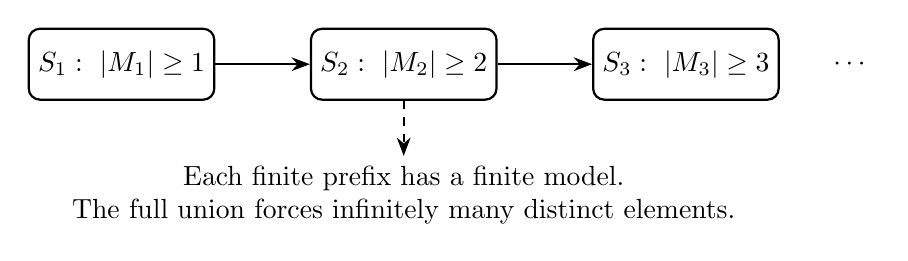
\begin{tikzpicture}[>=Stealth,thick,node distance=1.7cm]
\node[draw,rounded corners,minimum width=2.2cm,minimum height=.9cm] (a) {$S_1:\ |M_1|\ge1$};
\node[draw,rounded corners,minimum width=2.2cm,minimum height=.9cm,right=1.2cm of a] (b) {$S_2:\ |M_2|\ge2$};
\node[draw,rounded corners,minimum width=2.2cm,minimum height=.9cm,right=1.2cm of b] (c) {$S_3:\ |M_3|\ge3$};
\draw[->] (a) -- (b);\draw[->] (b) -- (c);
\node[right=0.55cm of c] (d) {$\cdots$};
\node[below=0.7cm of b,align=center] (e) {Each finite prefix has a finite model.\\The full union forces infinitely many distinct elements.};
\draw[->,dashed] (b.south) -- (e.north);
\end{tikzpicture}
\caption{The finite-stage illusion: coherent finite witnesses need not have a finite cumulative limit.}
\end{figure}

Every stage in this example is explicit and elementary. The obstruction is not contradiction: infinitely many pairwise distinct constants may be realized in an infinite model. The failure is finiteness of the limit. A finite-model search that works at all finite stages is therefore inadequate as a uniform proof that the total cumulative model remains finite.

\subsection{Undecidability of a finite-limit bound}
The bounded-witness theorem is exact but may be nonconstructive. One might hope that, for an effective sequence whose each finite stage has a small explicit model, an algorithm can decide whether a uniform cardinal bound exists. The next result rules this out in general.

\begin{theorem}[Undecidability of a finite cumulative model]\label{w2:th:finundec}
There is an effectively presented class of monotone first-order increment sequences such that every finite prefix has a finite model and the question
\[
 \text{``Does the cumulative union have a finite model?''}
\]
is undecidable uniformly in the description of the sequence. The assertion remains true when every individual increment and finite-stage satisfiability witness is effectively computable.
\prooflink{w2:pr:finundec}
\end{theorem}

The reduction uses a machine $M$ that is run for $n$ bounded steps at stage $n$. As long as no halt has occurred, the increment forces another fresh constant to differ from all earlier ones. Once a halt is observed, the process ceases to demand fresh distinct elements. Every local stage is finite-model satisfiable; the cumulative union has a finite model precisely when $M$ halts. The result addresses a different question from the consistency of finite
gift stages; its proof is a standard kind of reduction from the halting
problem.

\begin{corollary}[No uniform finite-limit witness bound]\label{w2:co:bound}
In the one-sorted class of Theorem~\ref{w2:th:finundec}, no total algorithm can decide from the effective stage description whether there exists a finite number $B$ bounding the sizes of suitable models for all stages. In particular, a sequence of successful finite-model checks does not supply an algorithmically recognizable global bound.
\prooflink{w2:pr:bound}
\end{corollary}

This result must be distinguished from the \emph{last-gift} barrier of
Theorems~\ref{w0:thm:next} and~\ref{w0:thm:stop}. Those theorems ask whether another eligible gift exists and whether the process stops. Here gifts may continue indefinitely while the \emph{domain size demanded by their accumulated axioms} either stabilizes or grows without bound. The two decisions are different even when the same halting mechanism exhibits their undecidability.


\section{The horizon of knowing there is no next gift}\label{sec:horizon-braid}
The finite-limit question asks what kind of \emph{model} survives an
unbounded sequence. The last-gift question asks what kind of \emph{information}
can establish that there is no further admissible step. Both involve
universal claims, but they quantify over different objects. A cardinality
bound on models is not a code-index bound on gift candidates. The halting-time family of Theorem~\ref{w0:thm:next} already settles
uniform undecidability. We do not introduce a second independent
undecidability mechanism here. Instead, we \emph{classify} its search
problem by recursively enumerable degree and ask which stronger
presentations make local finality decidable. We then compare weak
pointwise tests with exhaustive child listings to see precisely where
additional information changes the conclusion.


\subsection{Extensional and effective finiteness}
\begin{definition}[Weak and strong gift presentations]\label{w3:def:presentations}
A \emph{weak effective gift presentation} is a natural-number input code $x$ and a total computable predicate $P(x,j)\in\{0,1\}$, where $j\in\mathbb N$ indexes a candidate gift expression and $P(x,j)=1$ means the contract is admissible at the selected stage. The presentation is \emph{extensionally locally finite} if $A_x=\{j:P(x,j)=1\}$ is finite. It need not come with a computable complete list of $A_x$.

A \emph{strong effective child presentation} of a rooted gift tree is a total computable function $L(v)$ returning a \emph{complete finite list} of the immediate child codes for every valid node $v$. A tree has no node with infinitely many listed children. Membership of a finite valid history is decidable by successive calls to $L$. The distinction concerns the supplied effective presentation, not the abstract number of children.
\end{definition}

In a weak presentation, evaluating any proposed expression is a finite algorithmic operation. Deciding that \emph{none} will succeed quantifies over an infinite computable catalogue. In a strong presentation, the finite list is accompanied by an algorithm that has already discharged the completeness obligation for that node.

\begin{definition}[Local discovery, finality, and witness rank]\label{w3:def:rank}
Write
\[
 E(x)\iff\exists j\ P(x,j)=1,\qquad F(x)\iff\forall j\ P(x,j)=0.
\]
For a positive instance define its \emph{first-witness rank} $\rho(x)=\min\{j:P(x,j)=1\}$. A \emph{computable completeness horizon} for the family is a total computable $b(x)$ such that, whenever $E(x)$ holds, $\rho(x)\le b(x)$. For negative instances the bound is vacuous; $b$ does not purport to certify them without checking the finite initial segment.
\end{definition}

The witness rank measures \emph{how far the search must inspect the grammar's codes}, not the number of atoms or legal moves, the length of a formal proof, or the time needed to execute a gift. A machine may find at most one applicable gift after a very long search over unsuccessful names.

\begin{theorem}[Computable completeness-horizon criterion]\label{w3:th:horizon}
For a uniform family given by a total computable candidate predicate $P(x,j)$, the following are equivalent:
\begin{enumerate}[label=\textup{(\alph*)}]
\item There is a total computable decision procedure for $E(x)$.
\item There is a total computable completeness horizon $b(x)$ for the first-witness rank.
\end{enumerate}
This equivalence does not depend on whether $A_x$ is finite, although it is particularly informative when every $A_x$ is finite.
\prooflink{w3:pr:horizon}
\end{theorem}

This exact criterion makes the missing assumption explicit. Finitely many admitted children do not supply a computable bound on the index of the first possible child. But any algorithm deciding local emptiness implicitly supplies such a bound by searching for a witness after answering that one exists. Conversely, a bound and total candidate checks make a finite exhaustive search possible.

\begin{corollary}[An effective atom cap is not enough]\label{w3:co:atom}
Even if every gift uses a single atom, every candidate is decidable, and each instance has at most one admissible next gift, a computable completeness horizon need not exist. A finite numerical cap on the number of distinct atom names bounds accepted \emph{depth}, not candidate-code rank.
\prooflink{w3:pr:atom}
\end{corollary}

\subsection{The r.e./co-r.e. local frontier}
We use the standard terminology \emph{recursively enumerable} (r.e.) for a set whose positive members can be listed or semi-decided, and \emph{co-r.e.} for the complement of an r.e. set. A set is \emph{r.e.-complete} here if every r.e. set is computably many-one reducible to it; co-r.e.-completeness is dual. This is only a classification of a specified family of effective descriptions, not an assertion about all imaginable gifts.

\begin{theorem}[Local discovery and finality occupy dual classes]\label{w3:th:dual}
For every fixed uniform total computable candidate predicate $P(x,j)$, the existence set $E=\{x:\exists j\,P(x,j)=1\}$ is r.e. and its complement $F$ is co-r.e. Moreover, there exists an explicitly uniform total computable predicate $P_*(x,j)$ for which every $A_x$ has at most one element, yet $E_*$ is r.e.-complete and $F_*$ is co-r.e.-complete. Thus singleton branching does not guarantee decidable local finality. Completeness refers to this constructed worst-case family, not to every decidable admission predicate.
\prooflink{w3:pr:dual}
\end{theorem}

This strengthens Theorem~\ref{w0:thm:next}, rather than repeating its
conclusion: the \emph{same} first-halting-time reduction supplies the
completeness lower bound, while enumeration of the total candidate tests
supplies the upper bound. A positive gift has a finite discovery witness;
a negative finality claim still quantifies over every candidate code.

\begin{corollary}[Uniform finite finality certificates cannot be complete]\label{w3:co:cert}
For the constructed complete family $P_*$ of Theorem~\ref{w3:th:dual}, there is no total computable predicate $R(x,c)$ on finite proposed certificate codes $c$ such that
\[
 F(x)\quad\Longleftrightarrow\quad\exists c\,R(x,c)=1.
\]
In particular, no uniform finite certificate format with decidable checking can be both sound and complete for every true finality claim in that family.
\prooflink{w3:pr:cert}
\end{corollary}

The corollary does not prohibit a proof for a particular terminal stage. It rules out a \emph{uniform complete} method under the precise assumptions. The phrase ``Player 0 might already have its last gift'' must never be read as ``no particular last gift can be established.''

\subsection{Strong listing and unbounded-depth completion}
Now strengthen the presentation: each node of the rooted tree comes with a total computable, exhaustive \emph{finite} child list. The local question is trivial to decide by checking whether the returned list is empty. But a different limit question remains.

\begin{theorem}[Effective local completeness does not decide global completion]\label{w3:th:tree}
Consider a uniform effective description of rooted finite-history trees, with a total computable complete finite child-list function $L(x,v)$ at every valid node $v$ of instance $x$. Then:
\begin{enumerate}[label=\textup{(\roman*)}]
\item Whether a specified node is terminal is uniformly decidable.
\item The set of instances whose reachable trees are finite is r.e.; its complement is co-r.e. There exists an explicit such uniform family for which these sets are respectively r.e.-complete and co-r.e.-complete.
\item By K\"onig's lemma, in these finitely branching trees the tree is infinite if and only if it has at least one infinite branch. Thus a complete local child listing does not guarantee a decision procedure for the existence of an infinite gift history.
\end{enumerate}
\prooflink{w3:pr:tree}
\end{theorem}

This theorem locates a \emph{second} Last Gift obstruction. With a weak presentation, a stage's lack of further admissible gifts can be undecidable despite only one possible child. With a strong presentation, that local question is decidable, yet discovering whether a full process with arbitrarily many stages always completes is undecidable. The two are not interchangeable.

\begin{figure}[htbp]\centering\small
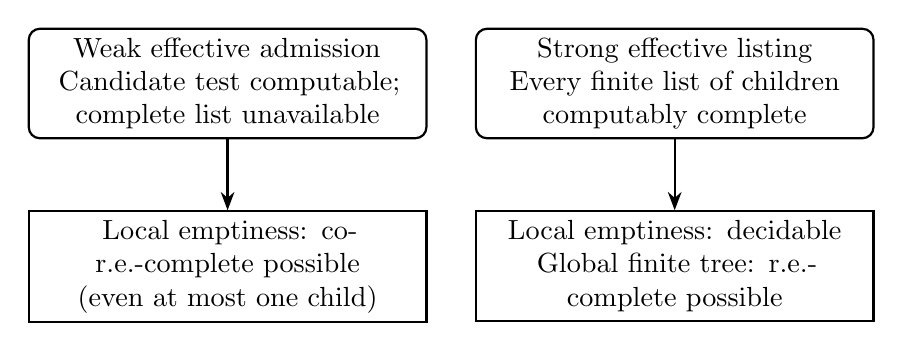
\begin{tikzpicture}[>=Stealth,thick,node distance=1cm]
\node[draw,rounded corners,align=center,text width=4.75cm,minimum width=5.05cm,minimum height=1.2cm] (w) {Weak effective admission\\Candidate test computable; complete list unavailable};
\node[draw,rounded corners,align=center,text width=4.75cm,minimum width=5.05cm,minimum height=1.2cm,right=0.6cm of w] (s) {Strong effective listing\\Every finite list of children computably complete};
\node[draw,align=center,text width=4.75cm,minimum width=5.05cm,below=0.9cm of w] (we) {Local emptiness: co-r.e.-complete possible\\(even at most one child)};
\node[draw,align=center,text width=4.75cm,minimum width=5.05cm,below=0.9cm of s] (se) {Local emptiness: decidable\\Global finite tree: r.e.-complete possible};
\draw[->] (w) -- (we); \draw[->] (s) -- (se);
\end{tikzpicture}
\caption{Two different completeness horizons. The stronger local information moves the undecidability from immediate emptiness to global depth.}
\end{figure}

A fairness or scheduling assumption does not eliminate these logical distinctions. The B15 counterexample already shows that the ability to act and the guarantee of being scheduled are separate. Here even with perfectly reliable execution of every local test, the issue is the unavailable uniform global answer.

\begin{theorem}[Finite depth plus complete listing yields total reconstruction]\label{w3:th:cap}
Suppose an effective gift tree has a complete computable finite child-list function and a known finite bound $m$ on the depth of every branch, for example the $n$-distinct-atom gift rule together with a fixed atom set of size $m$. Then an algorithm constructs the entire finite tree, its terminal nodes, and its maximum realized depth. No additional global halting oracle is needed.
\prooflink{w3:pr:cap}
\end{theorem}

Notice the exact assumptions: a \emph{known bound} and a \emph{complete, terminating child-list algorithm}. Dropping either changes the computability picture. With weak presentation, depth may be at most one and local emptiness still undecidable. With strong presentation but unbounded depth, eventual completion still undecidable.

\subsection{Certificates and the two-axis frontier}
The logical burden in a negative answer is not a consistency certificate for an individual gift: it is evidence covering an entire set of alternatives. A suitable local proof object may therefore contain a declared finite search domain, the complete enumeration of all permissible candidates within that domain, and a proof that no permissible candidate lies outside it. If candidate checking is decidable, these ingredients yield a machine-checkable finality certificate for that \emph{specific} stage. Theorem~\ref{w3:th:dual} shows why a universal producer of such objects cannot cover every terminal stage in the weak class.

\begin{definition}[Certified complete local frontier]\label{w3:def:frontier}
For a weak presentation $x$, a \emph{complete local frontier witness} is a natural number $b$ together with a sound proof (in an explicitly specified verification system) that
\[
 \forall j>b\quad P(x,j)=0.
\]
A checker also verifies $P(x,j)=0$ for each $j\le b$. If both components pass and the proof system is sound for the displayed assertion, the stage is final. This is a \emph{sufficient certificate shape}, not a promise that every final stage possesses such a certificate in one effective proof system.
\end{definition}

\begin{proposition}[Soundness of certified frontiers]\label{w3:prop:frontier}
Under a sound checker for the bound-exhaustion assertion and total correct individual candidate tests, any accepted complete local frontier witness proves $F(x)$. Completeness for all true $F(x)$ is impossible for the hard weak family of Theorem~\ref{w3:th:dual} if frontier certificates are effectively enumerable and verification is decidable.
\prooflink{w3:pr:frontier}
\end{proposition}

\begin{table}[htbp]\centering\small
\begin{tabularx}{\textwidth}{@{}p{0.28\textwidth}X X@{}}\toprule
Information supplied & Local finality & Entire tree finite? \\ \midrule
Decidable tests of all candidates; actual next-gift set finite & co-r.e.-complete in a hard family & Not settled by the local hypothesis \\
Computable complete list of immediate children & decidable & r.e.-complete in a hard family \\
Complete child list and a known depth bound & decidable & decidable by exhaustive finite traversal \\
\bottomrule\end{tabularx}
\caption{The completeness frontier: exact hypotheses rather than an unrestricted claim of last-gift decidability.}
\end{table}

This classification gives a practical design principle for formal research protocols: report \emph{provisional exhaustion} when search ended without a proof of completeness, and \emph{certified exhaustion} only when the entire permitted candidate domain has been accounted for. It does not imply an installed autonomous theorem prover or an actually run AMLD+0 federation.



\section{The shortcut question revisits the gift tree}\label{br:sec:shortcut-bridge}
The completeness horizon says that no finite search certificate can generically recognize the final admissible gift. A different question is whether a \emph{particular} finite composition can reduce the cost of reaching a declared goal. The research note on shortcuts makes several such conjectures without claiming that the source atoms already implement them. We link this line to verifiable self-improvement only after distinguishing certificate validity from economic or computational benefit.


\section{Verifiable self-improvement under sovereign gifts}\label{br:sec:mvsi}
\noindent\textit{Integrated from the original Verifiable self-improvement under sovereign gifts research note, November 21, 2026. The exact source filename and bytes are retained in the accompanying preservation archive.}

\begin{quote}\small\textbf{Source abstract (preserved).} The Mathematics of Verifiable Self-Improvement (MVSI) asks not merely whether a mathematical discovery system can become more effective, but whether its revisions can be authorized, certified, inherited, and evaluated without silently changing what counts as established mathematics. Earlier work on generalized board games (GBG), board-player extensions (GBG+), AMLD+0, verifier-gated dreaming, and self-improving discoverers supplies concrete results on proof reachability, passive extension, certificate inheritance, scheduler fairness, and fully charged improvements. We investigate a possible next layer, GBG+S: a proposed system in which the \emph{original} GBG+ Player~0 remains the unique sovereign and may receive guarded gifts changing aspects of the operational system. This article does \emph{not} assume that a fixed formal GBG+S theory has been shown consistent, that its gifts are universally representable as mobility, or that any proposed gift is automatically admissible. Instead, we formulate explicit conditional preservation results for mixed move-and-gift histories, conservative proof-rule upgrades, bounded service fairness, and successor handoffs; prove a finite-gift settlement-transfer statement; exhibit counterexamples to careless claims; and identify specific existing theorems that a sovereign-gift semantics could generalize. The central proposed contribution is a theory of \emph{certified changes to the conditions of certified mathematical discovery}, rather than a grant of new mathematical truth by authority.\end{quote}





\textbf{Keywords:} GBG+S; GBG+; XYZ formal systems; mathematical self-improvement; automated theorem proving; AMLD; verifier succession; typed evidence; sovereign gifts; relative consistency.


\subsection{The precise opportunity}
The current corpus already connects legal game moves to partial unary inference rules, legal histories to finite proof traces, and proof-search control to the distinguished board-player of GBG+~\cite{mvsi:GBG,mvsi:GBGp}. An AMLD+0 architecture puts the five settlement roles $P,R,D,I,C$ under a Player-0 scheduler while retaining verifier-governed BANK admission~\cite{mvsi:AMLD0}. A later discoverer paper separates theorem inheritance, inheritance of \emph{discovery methods}, and charged evidence of improved search~\cite{mvsi:Successor}. These are actual research results and architectural definitions; none requires a sovereign who can rewrite the rules of the host game.

GBG+S proposes asking a stronger question: \emph{What if the original Player~0 can be granted carefully delimited powers to revise the system in which the ATP or AMLD searches?} A revision might install a checked derived-rule macro, alter the schedule, change representation, delegate execution, or attempt a verifier succession. Some are plausible; others are forbidden or remain undecided in the current research protocol. The useful mathematics is therefore the \emph{boundary}: which properties must be preserved and what additional proof obligations appear when the rules themselves become state-dependent?

The analogy with research conditional on the Riemann hypothesis is appropriate only with care. The working hypothesis is not that every imaginable sovereign action works. Rather, one seeks two distinct kinds of claims: a relative-consistency hypothesis, and theorems derived only after a particular gift contract has been formalized. For example, one may target statements of the form
\begin{equation}\label{mvsi:eq:conditional}
\left[\Con(T_{+})\Rightarrow\Con(T_{S})\right]
\quad\text{and}\quad
\left[T_S+\mathcal H_g\right]\vdash\mathcal P_g,
\end{equation}
where $T_{+}$ is a \emph{specified} formal GBG+ theory, $T_S$ a \emph{specified} GBG+S extension, $\mathcal H_g$ an operational contract for a permitted gift, and $\mathcal P_g$ a preservation or improvement claim. Neither half of~\eqref{mvsi:eq:conditional} has been proved in general merely by naming GBG+S. In particular, $\Con(T_S)$ does not entail that a given gift is authorized, that every certificate checker is sound, or that a self-revision has positive value. Structural existence, syntactic consistency, semantic soundness, and effective admission are different obligations.

\subsection{A provisional sovereign-gift interface}
\begin{definition}[Epoch configuration]\label{mvsi:def:epoch}
For this article only, a complete epoch is a record
\[
X_e=(Q_e,F_e,V_e,B_e,\sigma_e,A_e,C_e,H_e,S),
\]
where $Q_e$ contains the rule-complete ordinary search/game state and its resource ledger, $F_e$ is the object proof calculus, $V_e$ its versioned certificate-checking interface, $B_e$ a typed provenance-bearing BANK, $\sigma_e$ a legal service/control schedule, $A_e$ the authorization data, $C_e$ cumulative commitments and theory constraints, $H_e$ the authenticated history, and $S$ the \emph{unique original} GBG+ Player~0. A candidate gift is a partial transition $g:X_e\rightharpoonup X_{e+1}$ with declared changed coordinates and a checkable evidence packet whenever one is available. We distinguish ordinary legal player moves $X\xrightarrow{m}Y$ from activated gift transitions $X\xrightarrow{g,w}g(X)$. The latter occur only after the appropriate external admission gate is passed. A rejected or unresolved proposal may also produce an administrative audit-log update $X\xrightarrow{a}Y$; this is neither an activated gift nor a legal player move, and it cannot by itself complete a game.
\end{definition}

This is a \emph{proposed interface}, not a claim that these data and rules already constitute the finalized axioms of GBG+S. It is chosen to expose the obligations relevant to MVSI. In particular, a gift is not identical to an ordinary theorem-proving move; gifts may change the admissible next-move relation.

The current sovereign-gift requirements are treated as constraints on any later formalization. A proposed gift is not presumed to be beneficial, and the availability of an ordinary move does not imply an unrestricted gift permission:
\begin{enumerate}
\item $S$ is the original GBG+ Player~0; delegated executors, copies, and promoted agents do not silently become additional sovereigns.
\item Ordinary GBG+ obligations survive an authorized gift, and logical consistency is judged externally, not by $S$'s declaration.
\item STOP rejects a gift incompatible with the \emph{cumulative} admitted history; an undetermined check never licenses activation.
\item Permissions, provenance, prior commitments, and versioned certificate scopes are explicit. A proposed change of verifier is not automatically lawful.
\item A completed game contains at least one actual legal player move (possibly by $S$). A zero-move STOP history is not reclassified as a completed game.
\end{enumerate}
A sound sufficient admission certificate need not be a complete decision procedure for consistency. Treating STOP as a uniformly terminating decider for arbitrary effectively presented first-order theories would contradict the general undecidability of their consistency problem. Thus \emph{rejection} supported by an incompatibility witness and \emph{withholding activation} because an obligation is unresolved are distinct outcomes. Neither is permission to proceed.

\begin{definition}[Evidence-qualified admission]\label{mvsi:def:admit}
Relative to a fixed proposed contract $K$, write $\Adm_K(X,g,w)$ when an external checker accepts evidence $w$ for all declared obligations: authority, cumulative compatibility, the identities of rules and verifiers, dependency preservation, and the selected safety invariants. The claim that this gate is \emph{sound} is an independent hypothesis about the checker and what $w$ certifies; it does not follow from the gate returning an acceptance bit. A candidate for which no adequate evidence is presently available is \emph{not activated}. A failed proof search alone is not a proof of inconsistency.
\end{definition}

\subsection{Conditional preservation results}
\begin{theorem}[Mixed-history sovereign-gift invariant preservation]\label{mvsi:thm:invariant}
Fix a transition contract $K$ and an invariant $I(X)$ on complete, versioned epoch configurations. Assume:
\begin{enumerate}[label=(\roman*)]
\item $I(X_0)$ for the initial configuration;
\item every reachable ordinary player move $X\xrightarrow{m}Y$ and every audit-only step $X\xrightarrow{a}Y$ preserves $I$, whenever $I(X)$ holds;
\item every activated gift $X\xrightarrow{g,w}Y$ satisfies $Y=g(X)$, has an admitted certificate $\Adm_K(X,g,w)$, and its sound transition obligation establishes
\[
I(X)\wedge\Adm_K(X,g,w)\Longrightarrow I(Y);
\]
\item every realized transition is one of these three kinds; unresolved or rejected proposals never activate a gift and any administrative logging is covered by (ii).
\end{enumerate}
Then $I$ holds after every finite legal mixed history of ordinary moves, audit-only updates, and activated gifts. This includes histories with schedule or proof-search changes satisfying the same obligations.
\end{theorem}
\phantomsection\label{br:mvsi:stmt:1}\prooflink{br:mvsi:proof:1}


The theorem is elementary but architecturally consequential. It turns the phrase ``safe self-improvement'' into an explicit \emph{transition-preservation obligation}. A useful instance is the \emph{live-proof-checkability} invariant (assuming records contain a type tag):
\begin{equation}\label{mvsi:eq:ledger}
I_{\rm proof}(X):\quad
\forall r\in\Live(B_X),\ \operatorname{type}(r)=\mathsf{PROOF}\ \Longrightarrow\ 
\exists p\;\bigl[V_X(p,r)=1\ \wedge\ \Prov_X(p,r)\bigr],
\end{equation}
\emph{together with} a separate assumption that the verifier is sound for its declared logic, hypotheses, and semantic scope. The witness $p$ must be checked against the record's own theory version and dependency context; if that version is no longer live, an archived record does not automatically qualify as a current premise. Without that soundness assumption, the mere existence of a checked string does not establish truth. Historical records may remain available with a changed status even when they can no longer be promoted as live mathematical premises.

\begin{corollary}[Conservative derived-rule gift]\label{mvsi:cor:macro}
Suppose a separately admitted sovereign gift retains all axioms and rules of an object calculus $F$ and installs only sound, finitely replayable $F$-derived macro-rule schemata, with identical theorem language, hypotheses, and applicable side conditions. For the resulting $F'$,
\[
\Gamma\vdash_{F'}\varphi\quad\Longleftrightarrow\quad\Gamma\vdash_F\varphi.
\]
The gift can change the cost and accessibility of a proof without changing the set of derivable sentences.
\end{corollary}
\phantomsection\label{br:mvsi:stmt:2}\prooflink{br:mvsi:proof:2}


\begin{remark}[No cost guarantee]
Conservativity does not entail a faster machine. Proposal generation, proof checking, installation, transport, memory, and future search must all be charged. The successor-discoverer paper gives a stronger break-even criterion under conditional per-episode bounds~\cite{mvsi:Successor}. For old lower bounds $\ell_i$, new upper bounds $q_i$, and a bound $B$ on all one-time additional expenses, an improvement follows if
\[
\sum_{i=1}^{N}(\ell_i-q_i)>B.
\]
The inequality is useful only if its bounds are themselves justified under all declared caching, reuse, and adaptation options.
\end{remark}

\begin{remark}[A tiny ATP instance]
Let $F$ have the unary rule $P(t)\Rightarrow P(f(t))$. A candidate macro $P(t)\Rightarrow P(f(f(t)))$ expands into two old steps. A checked installation conserves derivability, while it may reduce one class of search traces from two online steps to one. Whether it actually saves complete charged cost depends on the installation expense, replay/checking charges, repeated workload, and the old comparator's permitted caching. It is a \emph{conditional example}, not an admitted GBG+S gift or an observed speedup.
\end{remark}

\subsection{The clock-rewrite test: an actual AMLD consequence}
The \emph{Fundamental Theorem of Round-Robin AMLD Settlement} establishes eventual certified settlement when a finite settlement history is available under the paper's exact history compilation and \emph{inner branch-covering} fairness assumptions~\cite{mvsi:RoundRobin}. Its outer round-robin condition prevents inter-role starvation; it is not by itself enough to ensure every search branch is explored. GBG+S clock gifts must respect both distinctions.

A tempting but false claim is that every locally ``fair'' replacement schedule preserves global nonstarvation. The following is an abstract re-planning counterexample, \emph{not} a claim that such rewrites are admissible in a finalized GBG+S theory. Consider two always-enabled agents $P_1,P_2$. At each turn the sovereign announces a fair infinite continuation that serves $P_1$ now and $P_2$ next, but replaces that schedule before the next service. The realized infinite execution serves $P_1$ at every turn. Every announcement has a fair tail, while the actual history starves $P_2$.

\begin{lemma}[Uniform service-debt preservation]\label{mvsi:lem:debt}
Suppose an infinite execution has a fixed finite roster of ordinary players, each continuously enabled after some finite time. Suppose one uniform integer $b\ge 1$ holds across \emph{all} sovereign schedule rewrites: for each such player, every block of $b$ consecutive \emph{realized} ordinary service turns after its time of permanent enablement serves that player at least once. Then no such player is starved, regardless of the number of schedule rewrites.
\end{lemma}
\phantomsection\label{br:mvsi:stmt:3}\prooflink{br:mvsi:proof:3}


A finite counter-based controller can be designed to enforce the block guarantee for finite rosters, if the legal scheduler always has an admissible service action before any debt ceiling is breached. That is a \emph{separate implementability condition}. Even global nonstarvation is insufficient for the branch-covering hypothesis of~\cite{mvsi:RoundRobin}; a full sovereign settlement-preservation theorem must retain appropriate coverage within each role.

\begin{theorem}[Finite-gift settlement transfer under retained reachability]\label{mvsi:thm:settlement}
Let an initial effective, verifier-gated AMLD configuration $X_0$ have a finite legal history leading to a certified settlement of a fixed target $T$. Suppose an actual execution contains only finitely many activated gifts. Assume that every realized transition up to and including the last gift preserves the property
\[
R_T(X):\quad \text{there exists a finite legal, certificate-accepted settlement history from $X$},
\]
where preservation includes a checked translation if the certificate or state language changes. After the last gift, assume the resulting fixed AMLD epoch satisfies all hypotheses of the Fundamental Theorem of Round-Robin AMLD Settlement, including exact history compilation, verifier-backed settlement, and the \emph{inner} branch-covering fairness condition. Then the actual search eventually settles $T$ with an accepted certificate.
\end{theorem}
\phantomsection\label{br:mvsi:stmt:4}\prooflink{br:mvsi:proof:4}


The reachability-transport premise is substantive: a rule change may remove the only settling path even while its verifier remains sound. Similarly, endlessly alternating individually admissible schedule changes requires an execution-level fairness proof, not merely this finite-gift theorem.

\subsection{Verifier succession is the sharper boundary}
In \emph{Graduation Is Epistemic Handoff}, the Verifier-Sovereignty Theorem holds when graduate guidance or Player-0 control changes search but leaves all required verifiers and their acceptance rules unchanged~\cite{mvsi:Graduation}. DATA MIND 3.0 likewise separates heuristic and operational intelligence from the mathematical authority of verifier-accepted evidence~\cite{mvsi:DataMind}. The extension to a sovereign who may be \emph{offered} a verifier change is not automatic.

\begin{question}[Verifier-succession transport]\label{mvsi:q:verifier}
Given verifiers $V_e,V_{e+1}$ for potentially differing proof interfaces, can we exhibit a computable, checked proof translator $\tau_e$, a statement/context translator $\theta_e$, and a declared truth-preserving semantic relation such that every retained \emph{source-qualified} proof $p$ passes a sound target check,
\[
V_e(p,\Gamma_e\vdash\varphi)=1\quad\Longrightarrow\quad
V_{e+1}(\tau_e(p),\theta_e(\Gamma_e)\vdash\theta_e(\varphi))=1,
\]
with the translated hypotheses genuinely licensed in the successor, correct provenance, scope, and dependencies, and independently justified soundness of $V_{e+1}$? Under what contract may this constitute a sovereign gift?
\end{question}

The displayed formula is a \emph{desired bridge obligation}, not a general theorem. In particular, verifier succession is an unresolved atomic candidate in the current GBG+S investigation; unguarded verifier rewriting is not thereby accepted. Replacing a verifier with an accept-all program demonstrates the hazard: a new program may accept a false sentence without making that sentence true. Consistency of a formal description of the controller does not supply semantic soundness of its certificates.

\begin{proposition}[Conditional live-certificate transport]\label{mvsi:prop:transport}
Suppose a proposed handoff has a finite, acyclic, dependency-closed set of live source proof records. For each retained record, assume (i) its source proof and exact hypotheses are checked, (ii) a computable translator produces a target proof accepted by the successor's sound checker from appropriately authorized translated hypotheses, and (iii) the translated record retains its scope, dependencies, and provenance. Then every such migrated record may be designated as a \emph{target-qualified} live proof record without treating the sovereign's assertion as a proof. Source records lacking these witnesses must not be promoted on the strength of this proposition.
\end{proposition}
\phantomsection\label{br:mvsi:stmt:5}\prooflink{br:mvsi:proof:5}


This distinction also sharpens a concept from \emph{What Survives the Successor?}: preserving old proof receipts is weaker than preserving the \emph{method} by which the predecessor generates new candidates~\cite{mvsi:Successor}. A sovereign handoff worthy of MVSI should specify a proof translation, an executable trace translation, resource accounting, and a rollback or historical-status rule when evidence cannot be transferred.

\subsection{Applications to ATP and AMLD self-improvement}
\begin{enumerate}[label=\arabic*.,leftmargin=1.8em,itemsep=0.45em]
\item \textbf{Conservative derived-rule compilation and charged break-even}~\cite{mvsi:Successor}. Can an ATP-generated, checked macro be lawfully installed while preserving old proof access and charging all proposal, checking, installation, and search costs?
\item \textbf{AMLD+0 Passive-Rewiring Theorem}~\cite{mvsi:AMLD0}. Does a sovereign-controlled AMLD admit a certified projection back to the original five-role machine when sovereign gift authority is not used?
\item \textbf{Fundamental Round-Robin AMLD Settlement}~\cite{mvsi:RoundRobin}. Which combinations of realized service fairness, inner branch coverage, and reachability transport survive clock gifts? Which instances satisfy Theorem~\ref{mvsi:thm:settlement}?
\item \textbf{Verifier-Sovereignty Theorem}~\cite{mvsi:Graduation}. Under which additional permissions and translations, if any, can verifier succession preserve accepted evidence without promoting authority into purported mathematical truth?
\item \textbf{Type-safe dreaming and waking}~\cite{mvsi:Dreaming}. Which gifts let evidence survive waking, changed roles, copied executors, and versioned BANK updates without turning an AUDIT or EVAL record into a PROOF record?
\item \textbf{XYZ/GBG structural encoding}~\cite{mvsi:GBG,mvsi:GBGp}. Can provisional MOBILITY and GRANT gifts, kept logically distinct, be encoded as finite paths without creating a second sovereign?
\end{enumerate}

These are \emph{test cases}, not six consequences already derived from GBG+S. They provide falsifiable obligations and minimal countermodels. For example, a gift preserving a certificate checker but violating inner branch coverage can break eventual settlement despite never accepting a false theorem. A gift preserving all logical theorems but losing a successor's candidate-generation procedure can fail the goal of continued self-improvement.

\subsection{Does a fragment of XYZ explain the sovereign layer?}
The GBG formalization encodes complete game states as well-formed objects and legal moves as partial unary inference rules inside an $XYZ$ formal system $F=(x,y,z)$~\cite{mvsi:GBG,mvsi:GBGp}. The GBG+ foundation already provides an explicit \emph{passive} extension $E$ and projection $U$ satisfying $U\circ E=\mathrm{id}$ on ordinary GBGs~\cite{mvsi:GBGp}. This is a structural preservation result, not an automatic syntactic consistency theorem for a sovereign theory.

The proposed next step is to ask whether \emph{active, admissible} GBG+S histories have a faithful rule-complete $XYZ$ encoding. The retained \emph{MOBILITY} and \emph{GRANT} candidates remain provisionally defined; a composite GRANT+MOBILITY is not the same as assuming that S already possesses mobility. If the ordinary inference rules themselves can be rewritten, the encoded complete state must include their current version and the gift-admission protocol. A faithful encoding must preserve unique $S$, cumulative constraints, authorization, the distinction between proposal and installation, observable effects, and the legal-move relation. If a legal gift has an effect that cannot be represented by a finite path of such complete states, the universal representation conjecture fails in that formulation.

One possible semantic target is a model construction
\[
E_S:\operatorname{Mod}(T_+)\longrightarrow\operatorname{Mod}(T_S)
\quad\text{with}\quad
U_S(E_S(M))\cong M.
\]
Constructing a suitable $E_S$ under fixed axioms would support a semantic relative-consistency implication. The existence of the forgetful map $U_S$ alone would \emph{not} establish it. Any syntactic consistency conclusion also requires a specified proof calculus and a justified connection between syntactic and semantic claims.

A distinct long-range objective concerns elementary equivalence: two richer models might induce elementarily equivalent GBG-related \emph{reducts} while disagreeing about a statement not expressible in that reduct language. This would be an expressibility result, not automatically an independence theorem. In particular, two elementarily equivalent models in the full first-order language of set theory cannot disagree on GCH. This distinction prevents a tempting but invalid shortcut.

\subsection{A finite-first research program}
A productive first experiment needs no promise that every gift exists. It requires one \emph{fixed} GBG+S candidate contract and a small fully enumerated machine. The following order prioritizes the proposed mobility representation rather than assuming its truth:
\begin{enumerate}
\item \textbf{Freeze the formal layer.} Specify $T_+$, the candidate $T_S$, the exact game/XYZ language, and the difference between ordinary moves and gifted changes. Do not substitute a slogan for axioms.
\item \textbf{Prove or refute model existence.} Construct a passive sovereign extension first, then add one concrete gift. Separate structural nonemptiness from the target $\Con(T_+)\Rightarrow\Con(T_S)$.
\item \textbf{Test mobility first.} Define one legal MOBILITY transition on complete $XYZ$ configurations and, separately, the authority contract for any GRANT+MOBILITY composite. Require uniqueness of $S$, observable faithfulness, a legal ordinary move for completed games, and external cumulative consistency obligations. Record whether the model exists.
\item \textbf{Then test a macro gift.} Use a tiny ATP with a decidable checker, one new finitely replayable derived rule, and an exact charged ledger. Verify old proof preservation and compare charged search reach against a specified baseline. Do not assume the gift is authorized simply because the macro is conservative.
\item \textbf{Then test a clock gift.} Use a finite AMLD surrogate with roles $P,R,D,I,C$, explicit service debts, and a branch enumeration policy. Exhibit the re-planning starvation counterexample and verify a stronger invariant.
\item \textbf{Stress proof transport.} Make a deliberately invalid checker upgrade, require STOP to reject activation on sufficient evidence, and preserve a trace of the rejected attempt without crediting it as a completed game.
\item \textbf{Audit the resulting claims.} Record exact hypothesis scopes, executable transitions, proof witnesses, countermodels, costs, and unproved obligations. Distinguish finite checks from universal theorems.
\end{enumerate}
The program should also permit noncooperative games and legal sovereign acts that fail to improve performance. The goal is not to engineer improvement into every definition, but to characterize exactly when verifiable improvement is possible.

\subsection{Conclusion}
The distinctive contribution GBG+S \emph{could} make to MVSI is not unlimited sovereign power. It is an explicit mathematical treatment of revisions to the machinery that discovers, checks, remembers, schedules, and inherits proofs. Existing GBG+, AMLD, and ATP research already provides the baseline theorems. The sovereign layer asks which of these theorems remain invariant under authorized changes of the game itself, and what new obligations such changes create.

The nearest useful results are modest but precise: mixed legal histories preserve an invariant when \emph{both} ordinary moves and certified gifts preserve it; and eventual AMLD settlement survives finitely many gifts only under explicit reachability transport and a final branch-covering regime. The substantial open work is to \emph{construct} interesting gifts satisfying this requirement, show that their controls have a consistent model, preserve the exact old proof and discovery methods that matter, and demonstrate a fully charged improvement. In this sense, GBG+S may become a mathematics of \emph{certified succession of mathematical discovery systems}; it is not yet such a completed theory.

\subsection*{Status and attribution}
This manuscript is an AI-assisted exploratory research draft prepared for the research director and subjected to an internal mathematical and document audit. The mixed-history invariant theorem, service-debt lemma, finite-gift settlement-transfer theorem, and conditional certificate-transport proposition are proved here from explicit assumptions; they do not prove the relative consistency of GBG+S. All global GBG+S claims, verifier-succession permissions, and universal XYZ-mobility representation remain open unless independently established. The listed earlier papers are primary sources for the \emph{existing} results, not endorsements of the proposed extension. No external peer review or formal proof-assistant verification is claimed.





\section{Trading, forking, clocks, and six atomic shortcut conjectures}\label{br:sec:short}
\noindent\textit{Integrated from the original Trading, forking, clocks, and six atomic shortcut conjectures research note, November 21, 2026. The exact source filename and bytes are retained in the accompanying preservation archive.}




\textbf{Status and scope.} The six entries below are \emph{proposed} GBG+S gift compositions saved from a research conversation. They are neither established primitive axioms nor certified admissible constructions. The familiar proof-by-cases rule is mathematically valid in classical logic, but its use as an actual B4+B11 operational shortcut still requires a faithful implementation and a measured benefit. The full relative-consistency transfer \(\Con(\mathrm{GBG+})\Rightarrow\Con(\mathrm{GBG+S})\) remains open.


\subsection*{Atomic vocabulary and the shortcut question}
This note uses the local induction label \(\mathrm{N{:}B1}=\text{MOBILITY}\), \(G=\text{GRANT}\), and historical catalogue identifiers \(\mathrm{H{:}B2}\) (Unlock--Revise--Relock), B4 (Fork), B9 (Resurrect), B11 (Cross-System Trade), B14 (Clock Rewrite), B19 (One Office, Many Executors), and B20 (Finite-Step Replication). Throughout this table B2, B4, B9, B11, B14, B19, and B20 without a prefix refer to \(\mathrm{H{:}B}\) catalogue numbers. \(\mathrm{N{:}B1}\) is MOBILITY, while historical \(\mathrm{H{:}B1}\) is Verifier Succession. These two unrelated B1 uses must not be conflated.

A \emph{shortcut} is not automatically an increase in theoremhood. It is an authorized composition that, for a specified task and a clearly priced resource model, returns a checker-accepted certificate or other permitted result at a lower cost than a declared baseline. We distinguish elapsed time, total computation, proof length, and cost of verification.

\subsection*{The six candidates}
\renewcommand{\arraystretch}{1.23}
\begin{center}\small
\begin{tabular}{@{}p{0.12\linewidth}p{0.25\linewidth}p{0.54\linewidth}@{}}\toprule
\textbf{ID} & \textbf{Atoms} & \textbf{Candidate shortcut}\\\midrule
S1 & B4 + B11 & \textbf{Proof shortcut.} Fork on a proposition, solve two assumption-scoped branches, and trade both valid proof certificates back for proof-by-cases.\\
S2 & B19 + B20 & \textbf{Parallel-time shortcut.} Replicate finite workers under a single sovereign office and search independent routes concurrently.\\
S3 & B2 + B11 & \textbf{Reusable lemma shortcut.} Import a checked certificate and install a provably conservative derived rule for repeated use.\\
S4 & B9 + B14 & \textbf{Checkpoint shortcut.} Restore a versioned checkpoint and reschedule work without silently erasing historical commitments.\\
S5 & N:B1 (MOBILITY) + G + H:B11 & \textbf{Access shortcut.} Reach an eligible system, authorize a trade, and import its certificate through a validated interface.\\
S6 & B4 + B19 + B11 & \textbf{Cooperative proof shortcut.} Assign scoped fork branches to separate executors, then reconcile checked results without merging incompatible assumptions.\\\bottomrule
\end{tabular}
\end{center}

\subsection*{First investigation: fork, then trade (S1)}
Let \(T\) be a theory in a classical proof system admitting proof by cases, and let \(\varphi,P\) be sentences. Suppose we obtain actual derivations
\[
  T\cup\{\varphi\}\vdash P
  \qquad\text{and}\qquad
  T\cup\{\neg\varphi\}\vdash P.
\]
Then the deduction theorem (or the proof-by-cases rule) yields
\[
  \boxed{T\vdash P.}
\]
\textbf{Reason.} From the left branch derive \(\varphi\to P\); from the right derive \(\neg\varphi\to P\). Classical excluded middle and case analysis now derive \(P\) in \(T\). The branch assumptions do \emph{not} become unscoped axioms of \(T\). In particular, unguarded import of \(\varphi\) and \(\neg\varphi\) would be inconsistent. A trade must preserve the certificates, their premises, and their scope.

\textbf{What remains to prove.} B4 must instantiate distinct, valid branches; B11 must move and replay the certificates in the recipient's checker; the composition must preserve cumulative sovereign-gift invariants; and a specified search/cost model must show a true shortcut. The display above proves the \emph{logical combination rule}, not these operational facts.

\subsection*{Parallel execution candidate (S2)}
For three independent tasks with execution times \(T_1,T_2,T_3\), one sequential schedule has elapsed time
\[
 T_{\mathrm{seq}}=T_1+T_2+T_3.
\]
Under a model with three genuinely concurrent workers and coordination overhead \(C\), an idealized elapsed-time estimate is
\[
 T_{\mathrm{parallel}}\approx\max\{T_1,T_2,T_3\}+C.
\]
This is a scheduling comparison, \emph{not} a theorem that B19 and B20 provide concurrency or decrease total computational work. A future implementation must account for worker creation, communication, resource budgets, branch overlap, proof checking, and arbitration by the one sovereign S.

\subsection*{Other candidates and their guards}
\begin{description}[leftmargin=0.12in,style=nextline]
\item[S3 --- Conservative rule reuse.] B11 may move a formally checkable derivation to another system. B2 may incorporate a derived rule only when that rule is justified relative to the recipient's accepted premises and checker. Exchanging uninterpreted strings is not exchanging proofs.
\item[S4 --- Checkpoint restoration.] B9 may designate an earlier version or runnable checkpoint. B14 may change clocks or schedules. Neither alone provides physical time travel, historical erasure, or a cost-free rollback. A safe composition must track the unchanged external event order and all recorded commitments.
\item[S5 --- Access and trade.] MOBILITY and GRANT may allow reachability and authorization; neither automatically establishes that a particular partner, certificate, or cross-system interpretation exists. Any received proof must be independently replayable in the recipient language.
\item[S6 --- Scoped cooperative proof search.] B4 may supply branches and B19 may supply executors; B11 can serve as a certificate-transfer interface. The unique sovereign remains one office, while local workers are not granted independent sovereignty. The receiving checker must explicitly validate the branch-discharge argument.
\end{description}

\subsection*{A testable composition conjecture}
For an eligible cumulative theory \(T\), task \(q\), and composite gift \(g\), define a candidate assertion
\[
\begin{gathered}
\Con(T)\Longrightarrow\Con(T+\Delta_g),\\[3pt]
\Vfy_T(\pi_g,q)=1,\qquad
\Cost_{\mathsf M}(g,q)<\Cost_{\mathsf M}(\mathrm{baseline},q).
\end{gathered}
\]
Here \(\Delta_g\) is an independently specified axiomatization of the gift, \(\pi_g\) a concrete replayable certificate, and \(\mathsf M\) a fixed cost model. The three claims are distinct proof obligations. \emph{Nothing in this note proves the conjunction for any of S1--S6.}

\textbf{Research priority.} Begin with S1 (B4 + B11) because its certificate-combination rule is already rigorous. Build a tiny proof-search case with two branch certificates, a deterministic receiver, complete provenance, and matched baseline costs. Then audit the extension's interaction with MOBILITY, GRANT, and the cumulative consistency ledger. S2 is a second candidate for an explicit elapsed-time experiment.

\subsection*{Preservation obligations for future AMLD+0 passes}
For each candidate, freeze the complete original theory and the gift's operational semantics; prove preservation of one sovereign S, declared rules, authorization, versioned history, and prior accepted axioms; prove that any proof accepted after trade has a finite checker-valid support graph; distinguish certificate validity from efficiency; and reject undetermined compatibility rather than activating it. The previously developed uniform preservation/induction theorem is useful \emph{only if} these actual hypotheses are discharged for the composed operation.

\smallskip\hrule\smallskip
\textit{Provenance.} This note records the six shortcut suggestions and the proposed B4+B11 experiment from the November 21, 2026 conversation. It is a research proposal and internal mathematical analysis, not an external or machine-checked proof, a real deployed federation, or authorization for background or paid computation.



\section{Temporal exchange is an open composition problem}\label{br:sec:temporal}
\textbf{A motivating proposal, not an adopted GBG+S axiom.} In the November 21 discussion, the research director proposed a round-trip exchange with a time-displaced, structurally identical system. Starting from internal clock reading $t$, the suggested sequence is
\[
 t\xrightarrow{\mathrm{H:B14}}t+k\xrightarrow{\mathrm{H:B11}}\text{trade}
 \xrightarrow{\mathrm{H:B14}}t\xrightarrow{\mathrm{H:B11}}\text{trade back}.
\]
The main aim is the \emph{second trade} at the original time: use a certified or otherwise permitted resource obtained during the excursion to shortcut some later acquisition or proof search. The related backward-time variant replaces $k$ by $-k$. A candidate second system may be an exact copy of the first system at a different clock position. These variants were exploratory and no permission to instantiate a future copy has been proved.

\paragraph{The missing semantics.} An operation $t\mapsto t+k$ changes a coordinate. It does not, without an additional lawful state-evolution or access axiom, perform $k$ units of computation or create a future knowledgeable counterpart. Likewise, $t\mapsto t-k$ need not restore a past snapshot. A proposed temporal-trade constructor must supply: (i) a complete, declared transition or versioned-state correspondence; (ii) an actual partner state accessible at the displaced time; (iii) compatible authorization and proof-language interfaces for both exchanges; (iv) an append-only or appropriately versioned evidence history preventing circular provenance; and (v) a cost calculation charging time displacement, counterpart computation, verification, and both trades.

\paragraph{A precise candidate target.} For a legal composite $g=\mathrm{TradeBack}\circ\mathrm{Return}_{-k}\circ\mathrm{Trade}_{t+k}\circ\mathrm{Shift}_{+k}$, one seeks a verified transition $X\xrightarrow{g}X'$ with equal initial and final internal clock coordinates but a new usable certificate or capability in $X'$, and then a genuine cost reduction versus an explicitly fixed baseline. Existence, consistency, and improvement are three different proof obligations. In particular, importing a proof whose only support is that very import would be cyclic and disallowed by the fixed verifier-gated provenance contract. The user-approved description is a \emph{research question}, not evidence of literal time travel or an established shortcut.

\section{Four obstacles on the road to sovereignty}\label{sec:four-barriers}
The argument has four distinct places at which a tempting implication fails.
These failures are related, but they cannot be collapsed. \emph{A legal transition} is not the same as a \emph{sound theorem}; \emph{separate consistency} is not \emph{joint compatibility}; \emph{finite models at each stage} are not a \emph{finite model of the union}; and \emph{a finite set of actual children} is not an \emph{effective certificate that every candidate has been considered}.
\begin{enumerate}[label=\textbf{\arabic*.},leftmargin=2.2em]
\item \textbf{Construction barrier.} Typed models of specified permissions exist in restricted GBG+ presentations, but a model of an operational gadget is not an interpretation of arbitrary GBG+S axioms.
\item \textbf{Composition barrier.} Independently satisfiable increments can be inconsistent in their union; common-base expansions on disjoint new signatures are sufficient for a gluing theorem.
\item \textbf{Limit barrier.} Classical compactness carries finite-stage satisfiability to a model of the union, but only a uniform finite cardinal bound forces a finite limit model.
\item \textbf{Completion barrier.} With weak admission predicates, even one possible child can conceal an undecidable finality question. An exhaustive computable child list decides local emptiness, not necessarily total finite-tree completion.
\end{enumerate}
The four distinctions suggest a \emph{joint obligation}: a proposed gift should be checked against a fixed external logic, supplied with typed operational semantics, tested against previously accepted gifts, and accompanied by a certificate of exhaustiveness whenever finality is claimed. This is a conditional design rule derived from the preceding theorems, not a proof that a universal procedure meets all four obligations.


\subsection{Consequences for the intended sovereign-board theory}
The results concern fixed classical metalanguage theories and specifically constructed permission families. They do not decide the original GBG+S relative-consistency conjecture. A full transfer would need an exact translation of every admitted sovereign gift into a monotone, versioned increment and a proof that the activated-game semantics are faithfully represented. They also do not show that finite operational hardware is required by an abstract mathematical game: an infinite first-order model is a legitimate mathematical structure, while a finite executable deployment is a different engineering requirement.

Three significant separations now stand together. First, an extension of \emph{some} predecessor model need not lift every predecessor model. Second, an old-language conservative extension can yield strictly new capabilities, and vice versa. Third, successful finite-stage model construction can coexist with an infinite-only limit. These facts constrain any claim that individually checked gifts automatically assemble into a finite, executable sovereign board.


\subsection{Two independent quantitative horizons}
The bounded-model criterion and the completeness-horizon criterion have analogous quantified forms but measure different things. In the model-theoretic criterion, a common $B$ bounds \emph{model cardinality} for all finite prefixes, yielding a finite limit model by compactness. Here a computable $b(x)$ bounds the \emph{first admissible gift's code index}, yielding an algorithm for local nonemptiness. Neither bound implies the other: one concerns semantics of structures; the other concerns search over candidate descriptions. A finite operational model can have a next-gift question of arbitrarily high code rank, and a decidable gift grammar can generate theories with no finite cumulative limit.

Equally, the complete-child-list theorem makes no claim about a fully axiomatized GBG+S. A faithful transfer would need exactly typed sovereign atoms, observational equivalence, a way to compute or recognize allowable candidates, and a proof that every encoded branch respects cumulative consistency under the fixed external logic. Those requirements are substantial. The central contribution here is a criterion for what it would take to \emph{certify completion}, not a declaration that completion is universally achievable.


\subsection{The settlement-geometry comparison}
The September 22 paper \emph{Cooperative Settlement Geometry} \cite{coop} studies prover/refuter cooperation, verifier-accepted BANK deposits, shortest-path settlement horizons, and the impossibility of a uniform ``last breakthrough'' detector in an explicit-premise proof-horizon family. Its central descent assumption is
\[
h_0\ge h_1\ge\cdots\ge0,\qquad h_i\in\mathbb N,\quad h_0<\infty.
\]
Only finitely many strict horizon drops can occur; yet the paper's halting reduction shows that a universal algorithm need not recognize the last one. One toy instance has a single possible drop $2\to1$, delayed until an encoded machine halts.

\subsubsection{Shared computability limits, different progress relations}
\begin{center}
\small
\begin{tabularx}{\textwidth}{@{}p{0.29\textwidth}X X@{}}
\toprule
&\textbf{Cooperative Settlement Geometry}&\textbf{Bottom-up gift construction}\\\midrule
Accepted object&Verifier-accepted lemma/BANK deposit&Composite capability gift and its admitted stage\\
Invariant&Frozen object-theory deductive closure, for conservative deposits&Cumulative theory consistency, plus declared preservation conditions\\
Change measured&Settlement horizon $h_{n+1}-h_n$&Nonredundant capability extension and next-gift existence\\
Last-event question&Will another strict horizon drop occur?&Does another admissible gift exist?\\
Known negative result&Published proof-horizon last-breakthrough reduction&Theorems~\ref{w0:thm:next}--\ref{w0:thm:stop} for a locally finite, support-indexed gift family\\
Transfer limitation&Full AMLD settlement transfer conditional on a suitable compilation&Unrestricted GBG+S transfer not established\\
\bottomrule
\end{tabularx}
\end{center}

They exhibit a common \emph{finite local verification versus global completion} divide. They are not literally the same process: a consistent gift need not shorten a proof, and a conservative BANK lemma need not enlarge a game's logical capabilities. Both also distinguish effective discovery from mathematical existence.

If matching activation maps and cost models are supplied, one can \emph{define} a gift-related horizon difference $H(H_{n+1},x)-H(H_n,x)$ on carefully matched target states. A negative difference would signify a horizon-improving gift. No such general match is fixed here, and no unconditional speedup is claimed.



\section{Integration ledger: what survives, what is missing}\label{br:sec:integration-ledger}
The following statements deliberately separate internal manuscript proofs from the much stronger intended result.
\begin{longtable}{@{}p{0.25\linewidth}p{0.36\linewidth}p{0.32\linewidth}@{}}
\toprule
\textbf{Strand} & \textbf{Established under stated hypotheses} & \textbf{Still missing}\\\midrule\endhead
Original W0--W3 braid & Typed finite models, conditional compatibility/induction, finite-limit and computability boundaries & Exact unrestricted sovereign theory and interpretation \\
Acyclic compatibility & Join-tree algorithm decides finite joint satisfiability and builds a witness & Faithful encoding of actual complete gift contracts \\
MOBILITY--GRANT & Uniform GRANT construction for GRANT-ready MOBILITY models & Universal readiness and full original GBG+S commitments \\
Indexed preservation & Exact first-order consistency criterion; conditional all-model induction and compactness transfer & Explicit, composable constructions for all actual atoms \\
Verifiable self-improvement & Conditional invariant, fairness, conservative-rule and transport statements & Certified real upgrades and full verifier-succession semantics \\
Six shortcut proposals & Classical proof by cases is valid; finite test plans are specified & Legal composite operators and measured cost improvement \\
Temporal exchange & A typed proposed protocol and explicit obstructions & Actual time-displacement access, partner semantics and noncircular trade \\
\bottomrule
\end{longtable}

\paragraph{Four unresolved global blocks.} (1) Fix the full GBG+S theory without weakening GBG+. (2) Complete all retained atom contracts, including MOBILITY, GRANT, clocks, trade, and verifier succession. (3) Construct a model expansion or proof-preserving interpretation for the full axioms. (4) Prove compatibility of authorization, verification, provenance, history, and composites. Acyclicity addresses a particular finite case of (4), not (1)--(3).

\paragraph{Admission and completion are different.} STOP blocks inconsistent or undetermined gifts from activation; completed games require at least one actual legal player move, potentially by $S$. The zero-gift STOP history is not a completed game. An infinite consistency-preserving theory need not itself be a playable completed game. These obligations are not removed by the present braid.

\section{What remains to be proved}\label{sec:status-braid}
The results below refer only to the model classes and effective presentations
specified in their statements. A result classified as proved is proved under
those hypotheses, not automatically transferred to unrestricted sovereignty.
\begin{longtable}{@{}p{0.32\textwidth}p{0.45\textwidth}p{0.15\textwidth}@{}}
\toprule
\textbf{Problem} & \textbf{Supported result and scope} & \textbf{Status}\\\midrule\endfirsthead
\toprule
\textbf{Problem} & \textbf{Supported result and scope} & \textbf{Status}\\\midrule\endhead
Gift grammar and cumulative consistency & Cumulative consistency is equivalent to finite-prefix consistency in a fixed finitary calculus; a finite atom supply bounds the number of admitted gifts. & Proved \\
Restricted sovereign permissions & Finite structural witnesses are given for B1/B8/B22; other B-atoms retain their original guards or unresolved status. & Restricted \\
Next-gift undecidability & Uniform next-gift and deterministic eventual-stopping decisions are undecidable in constructed effective classes. & Proved \\
Typed permission packages & Finite tagged-permission realizations and support-indexed prefixes have explicit structural models. & Restricted \\
Mutual compatibility & Disjoint-signature common-model gluing is sufficient; separate satisfiability does not guarantee a consistent union. & Proved \\
Stopping versus maximality & Rejection-triggered protocol STOP does not entail maximality of the actual admissible frontier. & Proved \\
Early STOP versus completion & Zero-gift S2/S3 protocol terminations may admit no move; they are not completed games. Universal completability of every terminated process requires stronger assumptions or a changed protocol. & Conditional obstruction \\
Cumulative induction & Cumulative admitted increments preserve consistency exactly under the stated finite-obstruction conditions; no uniform admission decision is claimed. & Conditional theorem \\
Proof-preserving interpretations & A total axiom- and rule-preserving translation transfers consistency by proof-line induction; a sovereign translation is not supplied. & Conditional theorem \\
Model extension and conservativity & Some-model extension, all-model extension, conservativity, and operational novelty must be distinguished. & Proved \\
Finite limits & For one-sorted cumulative first-order theories, a finite union model exists exactly when all prefixes have models bounded by one common finite size. & Proved \\
Effective finite-model bounds & Finite-limit model existence is undecidable for an effective class with finite witnesses at every stage. & Proved \\
Weak completion frontiers & Local existence is r.e.-complete and finality co-r.e.-complete for a constructed at-most-one-child family. & Proved \\
Strong completion frontiers & Complete finite child lists decide local emptiness but not uniformly whether an unbounded-depth tree is finite. & Proved \\
Certified frontier claims & Sound complete-frontier witnesses certify particular terminal nodes; no effective sound-and-complete format covers every terminal case in the hard weak family. & Conditional and proved \\
Full GBG+S & The sources do not supply a fully checked all-atom interpretation or a syntactic relative-consistency proof. & \textbf{Open} \\
\bottomrule
\end{longtable}


\subsection{Obligations for a future sovereign theory}
\begin{enumerate}
\item \textbf{Freeze the atom language and local branching.} Type each B1--B23 entry as an operator, guard, counterexample, or question. Define well-formed composite gifts and equivalence of capabilities, not merely names.
\item \textbf{Freeze two layers of logic.} Fix the external classical metalogic used for $\Con(\Stage_n)$, and separately define any changing $xyz$ object logics. Checker replacement must not retroactively redefine what past consistency certificates meant.
\item \textbf{State exact relative-consistency strength.} Decide whether admission needs one explicit model, a model-extension construction valid for \emph{every} predecessor model, an interpretation, or a syntactic proof of relative consistency. These are noninterchangeable.
\item \textbf{Specify witness-carrying gifts.} Each accepted composite gift should have immutable source atoms, interface types, activation rules, formal proof/model witnesses, provenance, and an interaction test against accumulated gifts.
\item \textbf{Make the two STOP causes distinct.} An inconsistent candidate invokes the specified protocol STOP; a proof that no admissible candidate exists invokes maximality STOP. Unknown is neither one. Zero-gift STOP is never called a completed game; any stronger requirement that every termination be completable needs new operational hypotheses or a changed protocol.
\item \textbf{Construct $H$ separately.} Dormant consistency does not prove that exercising all accumulated permissions preserves verification, liveness, authority uniqueness, or cost constraints.
\item \textbf{Seek a faithful reduction.} Determine which genuine sovereign atoms implement bounded simulation and unbounded gift composition with observable nonredundancy. Only then promote the restricted last-gift theorem to the intended GBG+S class.
\end{enumerate}


\subsection{Concluding perspective}
The bottom-up construction replaces an unverified assertion of total sovereignty with a sequence of mathematically scoped gifts. Typed contracts and compatibility tests permit restricted positive constructions; finite-limit arguments control the kind of model that may survive cumulative development; computability theorems expose two irreducibly different obstacles to declaring that all gifts are exhausted. A failed candidate is not proof of maximality, and a successfully modeled finite stage is not proof of finite completion. The intended unrestricted GBG+S relative-consistency question remains open.


\subsection{Where the chapter ends: compatible sovereignty}
We have not shown that every intended sovereign power can coexist in one
formal structure.  We \emph{have} constructed restricted games in which a
unique distinguished board-player exercises explicitly declared,
sovereign-like permissions without violating the formal GBG+ transition
requirements.  This makes an important distinction visible: the existence
of sovereignty as a \emph{compatible possibility} is not contradicted by
the present mathematics, but that possibility must not be confused with a
relative-consistency theorem for the unrestricted composite theory.

What remains is neither to call every candidate power a theorem nor to
reject sovereignty because one forbidden merge fails.  It is to find one
faithful common interpretation of the \emph{admissible} sovereign
operations---or to discover a genuine obstruction.  \emph{The existence of
such a structure is the next theorem we seek.}

\paragraph{Research provenance and verification.}
The mathematical development integrates the four W0--W3 source manuscripts;
those source files remain unchanged. The present work preserves distinct
hypotheses and inherited results, with references to their provenance in the
bibliography. All proofs are manuscript-level arguments, not independent
machine-checker certificates or peer review. The earlier internal revision separated protocol histories from gameplay, added a
zero-gift obstruction and a restricted positive moving witness, made dispatch
reachability explicit, and stated the deduction assumptions needed for the
finite-obstruction equivalence. The present ATLAS revision additionally corrects
the classification of no-move STOP records: they are permitted process
terminations, but never completed games under the frozen completion rule. These
are corrections to the stated restricted results, not a verified model of
unrestricted sovereignty. No external novelty or priority claim is made.





\subsection{Source-and-revision concordance}\label{br:sec:source-concordance}
The integrated manuscript uses the attached audited braid as its uncut structural spine. Where two versions of the same later article were attached, the audited revision is the main integrated reading while both historical versions are retained unaltered in the source-preservation archive. No assertion that two versions represent independent proofs is made. The attached source pairs are: the revised Boring Game braid (LaTeX and PDF); the Acyclic Sovereign Gift Compatibility Theorem (LaTeX and PDF); the Uniform MOBILITY--GRANT Extension Theorem (LaTeX and PDF); the audited Indexed Consistency note (LaTeX and PDF); and the original and audited Sovereign Gifts / Verifiable Self-Improvement drafts. The separately saved Six Atomic Shortcuts note (PDF and LaTeX) supplies the sixth distinct research strand. Each source remains separately accessible in the accompanying ZIP. The body text of each \emph{canonical distinct} research strand is preserved in this braid; editorial front matter and individual bibliographies have been merged into unified title/status and references rather than repeated as separate standalone documents.

\subsection{ATLAS v2 adversarial audit: correction ledger and residual obligations}\label{br:sec:atlas-audit}
The audit was performed against the attached PDF and LaTeX source, using the same
ChatGPT model and its own reasoning and programmatic checks; it is \emph{not}
independent peer review or formal kernel verification. Three corrections were
necessary. First, Definition~\ref{br:def:lifecycle}, Theorem~\ref{br:th:stop-liveness},
and their proof now distinguish permitted zero-gift \emph{protocol termination}
from a \emph{completed game}. The earlier wording that called a zero-move STOP
record ``completed'' contradicted the frozen completion rule; no-move records
are now correctly excluded from completed games. Second, the finite-limit
cardinality criterion, Theorem~\ref{w2:th:bounded}, is stated explicitly
for one-sorted first-order theories, the setting where its displayed size
sentence applies. Third, the shortcut table distinguishes local induction
\(\mathrm{N{:}B1}\) (MOBILITY) from historical \(\mathrm{H{:}B1}\)
(Verifier Succession).

The audit also checks theorem/proof link resolution and the generated PDF's
compilation and layout. These are useful checks, not mathematical completeness
certificates. Remaining obligations include faithful full GBG+S axioms,
independently specified atom contracts, joint compatibility witnesses, a
sound relative-consistency interpretation, external verification and actual
shortcut-cost measurements. None is marked discharged merely by this edit.

\section{The program continues: we are not done}\label{br:sec:not-done}
\begin{quote}\large\bfseries
WE ARE NOT DONE. The preceding results are mathematical progress, not the final sovereign gift theorem.\end{quote}
Our principal desired transfer remains
\[
 \Con(T_{\mathrm{GBG+}})\Longrightarrow\Con(T_{\mathrm{GBG+S}}),
\]
with the full theory and its faithful interpretation still needing construction. A correct general induction theorem is not a proof that every actual atom satisfies the inductive contract. The restricted GRANT-ready extension is not a proof for arbitrary GBG+S models. An acyclic finite constraint witness is not a certificate for every composite. A proof-by-cases shortcut is not by itself a measured improvement. A clock rewrite is not, by name alone, time travel.

A continuation worth attempting is to develop a complete atom interface for one concrete, legally executable composite (beginning with MOBILITY--GRANT and then Fork--Trade), assemble faithful constraints with a common witness, check original GBG+ projection and unique sovereignty, carry genuine verifier evidence forward, and compare fully charged cost with a fixed baseline. Only after these obligations have certificates should they become induction premises for subsequent atoms. Negative results, failed candidates, and unclear tests are part of the research record and are not erased by a more polished exposition.

\textbf{No claim of completion, no claim of external certification, and no arbitrary research endpoint.} The braid is a dated checkpoint in an ongoing research program, intended to be revised when new proofs, counterexamples, or definitions become available.


\appendix
\section{PROOFS}
\label{sec:all-proofs}\label{w0:sec:proofs}
The only formal proof appendix. Proofs are organized by their main-text statement order, including integrated research strands. Internal checking is not an independent proof certificate.
\subsection*{Source-preservation note}
Original source theorem and proof text is retained here and in the matching source archive. Repetitions reflect independent manuscript versions, not additional independent validation.
\subsection{Proof of Proposition~\ref{w0:prop:fork}: fork consistency and failed merge}\label{w0:pr:fork}
\textit{Back to \hyperref[w0:prop:fork]{statement}.}
\begin{proof}
Assume $T+\varphi$ is inconsistent. By the classical deduction theorem, $T\vdash\neg\varphi$, contrary to independence. Likewise, inconsistency of $T+\neg\varphi$ implies $T\vdash\varphi$. But the theory $T+\{\varphi,\neg\varphi\}$ proves a contradiction using these two added premises, regardless of whether $T$ previously proved either. The two consistent branch theories must therefore remain separately scoped; the unguarded merge is inconsistent.
\end{proof}


\subsection{Proof of Proposition~\ref{w0:prop:zip}: guarded zip}\label{w0:pr:zip}
\textit{Back to \hyperref[w0:prop:zip]{statement}.}
\begin{proof}
By deduction, the hypotheses give $T\vdash\varphi\to\psi$ and $T\vdash\neg\varphi\to\psi$. Classical excluded middle yields $T\vdash\varphi\lor\neg\varphi$. Elimination by cases then gives $T\vdash\psi$. Neither $\varphi$ nor $\neg\varphi$ has been incorporated as an unconditional axiom of $T$.
\end{proof}


\subsection{Proof of Proposition~\ref{w0:prop:finitude}: finite-step barrier}\label{w0:pr:finitude}
\textit{Back to \hyperref[w0:prop:finitude]{statement}.}
\begin{proof}
Let $N_0$ be finite and let $N_{i+1}$ be obtained from $N_i$ by adjoining a finite set $A_i$ and perhaps deleting or promoting members. Then $|N_{i+1}|\le |N_i|+|A_i|<\infty$. Induction gives finiteness at every finite $i$. A clock is not used in the induction. To obtain an infinite new population in four transitions one would have to violate the finitary-update premise, begin with an infinite population, or change the meaning of ``four transitions.''
\end{proof}


\subsection{Proof of Proposition~\ref{w0:prop:role}: mixed and homogeneous authority}\label{w0:pr:role}
\textit{Back to \hyperref[w0:prop:role]{statement}.}
\begin{proof}
Let $A$ have an element $a$ with $\neg S(a)$ and let every element of $B$ satisfy $S$. If $f:A\to B$ were an isomorphism in the language containing $S$, then $S(a)$ would hold exactly when $S(f(a))$ holds. But $S(f(a))$ is true in $B$, contradiction. Thus no $S$-preserving isomorphism exists. This says nothing about untyped graph isomorphism after forgetting the $S$ predicate.
\end{proof}



\subsection{Proof of Proposition~\ref{w0:prop:atom-witnesses}: selected finite atom models}\label{w0:pr:atom-witnesses}
\textit{Back to \hyperref[w0:prop:atom-witnesses]{statement}.}
\begin{proof}
For B1 choose $S_1=\{0,1,2\}$ and verifiers $V(0)=\{P_1\}$, $V(1)=\{P_1,P_0\}$, $V(2)=\{P_0\}$. Declare the only board-mode transitions $T(0)=1$ and $U(1)=2$, each authorized to $P_0$. Each is a partial function with a unique successor. Interpret the mathematical certificate checker as a fixed predicate independent of mode. The board-player is the same unique $P_0$ at all three modes; a designated inactive underlying ordinary game supplies the GBG+-1 projection and the fixed label function supplies GBG+-5. These finite data satisfy the relevant rule-completeness and authorization requirements. They do not imply checker soundness for an unspecified application.

For B8 take $S_8=\{0,1\}$ with a single authorized board operation $\mathrm{Abdicate}(0)=1$ and no returning transition. A Boolean attribute $\mathrm{Privileged}(0)=1$, $\mathrm{Privileged}(1)=0$ distinguishes the privilege; $P_0$ remains the unique distinguished board-player (abdication is of a discretionary power, not logically the existence of the unique board office). One-way irreversibility holds relative to the declared graph, not to arbitrary undeclared future override rules.

For B22 fix five ordinary officials $u_1,\ldots,u_5$ and two call kinds $c_1,c_2$. Let jurisdiction $J(c_1)=\{u_1,u_2,u_3\}$, $J(c_2)=\{u_2,u_4,u_5\}$, so their overlap is nonempty. Define fixed priorities $u_1\succ u_2\succ u_3$ for $c_1$ and $u_4\succ u_2\succ u_5$ for $c_2$. Take a report vector in $\{0,1,\bot\}^5$, where $\bot$ means no report. For each call kind, $\mathrm{Resolve}$ chooses the top-priority \emph{reporting} eligible official and returns that official's $0$ or $1$; if none reports, it returns $\bot$ (``no call''). This makes $\mathrm{Resolve}$ total even for missing or contradictory reports. Encode a distinguished start state, both call kinds, all $2\cdot3^5$ report inputs, and the resolved outcomes as finite complete states. Declare setup transitions from the start to each input state and one resolution transition from each input state to the uniquely determined outcome, with every transition explicitly authorized (for example, to $P_0$ as the formal arbiter). Thus even the start state has only finitely many applicable rules. All five officials are ordinary participants, leaving the unique board-player $P_0$ unchanged. This supplies a finite GBG+ transition presentation. None of these isolated models establishes that an arbitrary combined gift is consistent.
\end{proof}


\subsection{Proof of Theorem~\ref{br:th:stop-liveness}: first move and early STOP}\label{br:pr:stop-liveness}
\backlink{br:th:stop-liveness}
\begin{proof}
Take a consistent background theory $T_0$ in a language with a nullary
predicate $p$ and a first candidate $g$ with the stipulated one-atom support.
Let $\Delta(g)=\{p,\neg p\}$. Then $T_0\cup\Delta(g)$ is inconsistent
by propositional logic. By S2 the candidate is rejected and the last
accepted stage remains $G_1$, with no gift installed. Since the dormant
$G_1$ and its zero-gift activation $H_1$ have empty internal transition
relations by hypothesis, there is no possible actual move after the external
STOP decision. The resulting terminated process, together with an empty play
trace, is a \emph{protocol-terminated record}, proving (i), not a completed
game. For an independent S3 witness, use an effective grammar with a certified
empty set of first-gift candidates: S3 stops immediately, again at $G_1$.
For either record no legal internal transition can be executed; hence the
record has no extension satisfying the completed-game definition, proving
(ii). If a proposed stronger axiom preserves every one of these permitted
terminated records and demands a completed-game extension for each, the
specific zero-gift record violates it. This establishes the incompatibility
in (iii). The frozen rule that \emph{every completed game has a move} remains
intact and is not falsified by a record that is not completed. Nothing here
settles an unaxiomatized unrestricted sovereign theory.
\end{proof}


\subsection{Proof of Proposition~\ref{br:prop:moving-completion}: a restricted positive witness}\label{br:pr:moving-completion}
\backlink{br:prop:moving-completion}
\begin{proof}
Let the atom set be $\{a_1\}$ and let the deterministic external
constructor offer only $g_1=a_1$. Set $T_0$ to a consistent, stage-scoped
description of the dormant one-state game. Let $\Delta(g_1)$ assert, in a
separate activated-stage description, the declared rule
$\rho:s_0\mapsto s_1$ with nonempty authorization $\{P_0\}$.
Interpret the dormant state by a one-vertex graph with no transitions and
the activated game $H_2$ by the finite graph with vertices $s_0,s_1$
and precisely the authorized edge $s_0\xrightarrow{P_0,\rho}s_1$.
These stage-scoped assertions have an explicit common model, so S1
admits the first gift. A second gift would require two distinct atoms,
which do not exist; S3 therefore proves no further gift is admissible
and STOP occurs at $G_2$. Impose as an explicit \emph{additional}
completion convention that $H_2$ is activated and its sole legal first
move is executed. The single resulting completed history contains an
actual player move. The convention is stronger than S1--S4 alone;
therefore the construction establishes compatibility on a restricted
subclass but does not invalidate the earlier counterexample.
\end{proof}


\subsection{Proof of Proposition~\ref{w0:prop:atom-bound}: finite atom cap}\label{w0:pr:atom-bound}
\textit{Back to \hyperref[w0:prop:atom-bound]{statement}.}
\begin{proof}
If the atom set has exactly $m$ elements, every finite composition $g$ has $|\operatorname{supp}(g)|\le m$. The stage-$n$ rule requires $|\operatorname{supp}(g_n)|=n$. Thus $n\le m$ at every accepted stage. Local finiteness is unnecessary, and the proof gives only a numeric bound; deciding whether a candidate exists at an earlier stage may still be undecidable.
\end{proof}


\subsection{Proof of Theorem~\ref{w0:thm:konig}: the gift-tree branch}\label{w0:pr:konig}
\textit{Back to \hyperref[w0:thm:konig]{statement}.}
\begin{proof}
The root has finitely many children. Since there are descendants at arbitrarily large depths, at least one of its finitely many children has arbitrarily deep descendants. Choose such a child. Repeat the same reasoning inductively at each subsequent node; local finiteness makes the selection argument possible. This constructs an infinite sequence of nested nodes, hence an infinite branch. Nothing here produces a uniform effective selector or proves every branch infinite.
\end{proof}


\subsection{Proof of Theorem~\ref{w0:thm:finite}: finite-support equivalence}\label{w0:pr:finite}
\textit{Back to \hyperref[w0:thm:finite]{statement}.}
\begin{proof}
If the union $\Stage_\infty$ is consistent, every subset $\Stage_n$ is consistent: an inconsistent subset would already supply a proof of contradiction from the union. Conversely, suppose every $\Stage_n$ is consistent but $\Stage_\infty$ proves $\bot$. A formal proof is a finite sequence of formulas and invokes finitely many nonlogical axioms $\alpha_1,\ldots,\alpha_r$ from the union. Each $\alpha_i$ belongs to some increment $\Delta_{k_i}$. Put $N=\max_i k_i$ (if no nonlogical premises are needed, the empty baseline calculus itself is inconsistent). The same finite proof is a proof of $\bot$ from $\Stage_N$, contradiction. Hence the union is consistent. The argument requires fixed finitary proof rules; no conclusion about mutable, unaligned consequence relations is inferred.
\end{proof}



\subsection{Proof of Proposition~\ref{w0:prop:infinite}: infinitely many support-indexed gifts}\label{w0:pr:infinite}
\textit{Back to \hyperref[w0:prop:infinite]{statement}.}
\begin{proof}
Take the effective atom supply $\Abs=\{a_1,a_2,\ldots\}$. At stage $n$, the grammar offers exactly the one candidate $g_n=a_1\circ\cdots\circ a_n$, with support size $n$. Use one fixed external observation contract $\mathrm{Query}(j)$, under which a successful activated response on index $j$ is observable. After gifts $1,\ldots,n$, the registry is $R_n=\{1,\ldots,n\}$; an input $j\in R_n$ has a declared success transition and an input $j\notin R_n$ is rejected. The $n$th gift is a permission for index $n$, so its success was impossible at the previous stage. Each $R_n$ has a finite complete transition presentation for its supported successful contexts (plus a default rejection case); all such presentations use the same external query semantics, and every dormant $G_{n+1}$ still has no enabled internal play. A fixed first-order signature with stage-indexed registry predicates models all finite prefixes at once; to witness a finite prefix, interpret its finitely many registry assertions as specified and the remaining indices as unauthorized. This supplies a model for each $\Stage_n$, and hence $C_n=1$ for the stipulated axiom scheme. The nonredundancy witness is the changed success answer to the \emph{same query $n$} across the two adjacent activated games, not merely a new state label. The gift-construction tree has exactly one child per nonterminal node, hence is locally finite, while the chain continues indefinitely. The claim concerns an effective construction, not the full sovereign atom catalogue.
\end{proof}


\subsection{Proof of Theorem~\ref{w1:th:finite}}\label{w1:pr:finite}\backlink{w1:th:finite}
Let $S$ be the finite state set of the base GBG+ presentation, and fix one reachable base state $s_*$ (the initial state suffices). Form a finite state set consisting of $S$, an input state $q_j$ for each $j\in J$, and an outcome state $r_j$ for each $j\in R$. Include every declared transition of the base on its $S$ component. For each $j\in J$ declare a distinct partial unary dispatch rule $d_j:s_*\mapsto q_j$ authorized to $P_0$. For every $j\in R$ include the partial unary success map $\rho_j:q_j\mapsto r_j$, again with stipulated nonempty authorization. These explicitly authorized dispatches make the input states reachable; the installed outcome states are then reachable as well, assuming the original base is presented by reachable states. No transition is left unspecified. The unused, merely named symbols $r_j$ with $j\notin R$ need not be vertices in the current stage: their absence is exactly what the frozen query interface tests. Declare the same unique board-player $P_0$ and same label operator $F$; the permission rules are entirely declared, satisfying the no-extra-system-action requirement. If the presentation uses a dormant/active indicator, restrict the enabled move set to empty when dormant and to the displayed rules when active, using that indicator in each complete state. No enabled action is defined at a dormant state. For $j\in R$, $O_R(j)=1$, whereas if $j\notin R$ the observable is zero. Finite successive registry choices preserve finiteness and all rules remain partial functions. Restricting to $S$ and its internal transitions recovers the base; the additional dispatches do not retroactively become base-game moves. If a chosen GBG formalism demands all states be reachable from a unique initial state, the dispatch construction supplies the required reachability for these gadgets. This proves the stated \emph{structural} claim, without postulating a theorem about syntactic relative consistency of every GBG+ model.\qed


\subsection{Proof of Corollary~\ref{w1:co:support}}\label{w1:pr:support}\backlink{w1:co:support}
At gift index $n$, the expression $a_1\circ\cdots\circ a_n$ has support exactly $n$ and installs permission $n$. Its stage is realized by Theorem~\ref{w1:th:finite} with $J=\{1,\dots,n\}$ and $R=J$. For the common observation index $n$, the preceding registry gives $O(n)=0$ and the next gives $O(n)=1$. Exactly one successor is offered. A finite model exists for every fixed $n$, and every cumulative contract can be written with versioned predicates describing precisely that finite stage.\qed


\subsection{Proof of Theorem~\ref{w1:th:glue}}\label{w1:pr:glue}\backlink{w1:th:glue}
For every new nonlogical symbol in $D_i$, take its interpretation from $M_i$. Pairwise disjointness makes these choices unambiguous. Interpret $L_0$ exactly as in $M$. The resulting structure $M^*$ has the same domain and $L_0$ reduct $M$. Every sentence of $\Delta_i$ concerns only $L_0\cup D_i$ and is true because the corresponding reduct of $M^*$ is $M_i$. Thus $M^*\models T_0\cup\bigcup_i\Delta_i$, for finite or countable $i$. If every base model $M\models T_0$ can be expanded this way, every base-language semantic consequence of the enlarged theory holds in every model of $T_0$. First-order completeness makes it a deductive consequence of $T_0$; soundness supplies the other inclusion.\qed


\subsection{Proof of Proposition~\ref{w1:prop:conflict}}\label{w1:pr:conflict}\backlink{w1:prop:conflict}
Take a language with a nullary predicate $p$ and let $T_0$ be the empty set of nonlogical axioms. Let $\Delta_1=\{p\}$ and $\Delta_2=\{\neg p\}$. Each alone has a one-element model with the appropriate truth value of $p$. Their union proves a contradiction by propositional reasoning. This shows individual satisfiability, even by finite models, is not compositional satisfiability.\qed


\subsection{Proof of Proposition~\ref{w2:prop:lift}}\label{w2:pr:lift}\backlink{w2:prop:lift}
Use a base language with one unary predicate $P$ and no nonlogical axioms $T_0$. Let $S'=T_0\cup\{\forall x\,P(x)\}$. There is a one-point model interpreting $P$ as the full domain, so $E$ holds. But a one-point model $M\models T_0$ with $P$ empty cannot be expanded to satisfy $S'$ while preserving the old predicate $P$. Hence $U$ fails.\qed


\subsection{Proof of Theorem~\ref{w2:th:independent}}\label{w2:pr:independent}\backlink{w2:th:independent}
Take $L_0$ containing a designated individual $c$ and no permission predicate. Introduce a fresh unary predicate $Q$, and let $S'=T_0\cup\{Q(c)\}$. Every nonempty base model can be expanded by setting $Q$ true of $c$, so $U$ holds. For every $L_0$ sentence $\varphi$, if $S'\vdash\varphi$, every base model expands to $S'$, hence every base model satisfies $\varphi$, and completeness gives $T_0\vdash\varphi$; thus $K$ holds. Define the frozen operational observation to ask whether the new permission $Q(c)$ is enabled. Before installation the activated registry answers 0, after installation it answers 1. Conversely, in a base language containing $P(c)$, add the previously undecided axiom $P(c)$ while fixing the registry unchanged. The new axiom is a strict old-language theory extension, but no activated permission observation changes.\qed


\subsection{Proof of Theorem~\ref{br:th:inductive}: cumulative admission}\label{br:pr:inductive}
\backlink{br:th:inductive}
\begin{proof}
If $T_n$ is consistent, then every $T_k\subseteq T_n$ is consistent.
If all prefixes are consistent but some finite $F\subseteq\Delta_k$ satisfies
$T_{k-1}\vdash\neg\bigwedge F$, then $T_k$ proves both $\bigwedge F$
and its negation, contradicting consistency. Conversely suppose the
finite-obstruction property holds. Begin with $\Con(T_0)$. If $T_{k-1}$
is consistent but $T_k$ inconsistent, a finite contradiction proof from
$T_k$ uses a finite set $F$ of axioms from $\Delta_k$. The deduction
principle in the fixed classical calculus yields
$T_{k-1}\vdash\neg\bigwedge F$, contradicting the assumed property.
Induction on $k$ gives $\Con(T_n)$. First-order soundness and completeness
identify consistency with model existence at each prefix.
\end{proof}


\subsection{Proof of Corollary~\ref{br:co:chain}: finite and infinite chains}\label{br:pr:chain}
\backlink{br:co:chain}
\begin{proof}
The finite claim follows from the induction hypothesis at each step.
If the infinite union were inconsistent, some finite contradiction proof
would use axioms from only finitely many of its constituent stages;
they occur together in a sufficiently large consistent stage, a
contradiction.  This is the same finite-support argument as
Theorem~\ref{w0:thm:finite}.
\end{proof}


\subsection{Proof of Proposition~\ref{br:prop:interpret}: proof translation}\label{br:pr:interpret}
\backlink{br:prop:interpret}
\begin{proof}
Assume $T_+$ is consistent and $T_S$ proves $\bot_S$. Take a finite
source proof $\pi$. Induction on its line number shows that the
translation of every line is derivable in the target: axioms translate
to target theorems, and a source inference step translates to a valid
finite target derivation whose premises are available by the induction
hypothesis. Thus $T_+\vdash\tau(\bot_S)=\bot_+$, contradicting
$\Con(T_+)$.  The proof-line induction is the standard mechanism
made explicit in~\cite[Theorem~1.10]{depthsv2}; the additional
translation hypotheses are obligations of the present proposition.
\end{proof}


\subsection{Proof of Proposition~\ref{w1:prop:stop}}\label{w1:pr:stop}\backlink{w1:prop:stop}
Let $T_0$ be a consistent propositional background, use new nullary $p,q$, and offer two proposals at the same next-gift index: $u$ would add $\{p,\neg p\}$ and $v$ would add $\{q\}$ with a fresh enabled permission witnessing novelty. Both proposals can be encoded as expressions with the same required number of distinct atoms by choosing that number of atom names. $u$ fails classical consistency; $v$ has a model. A deterministic policy that tries $u$ first and stops at the failed proposal has stopped while $v$ remains available. Thus stop-on-failure is not an exhaustion proof.\qed



\subsection{Proof of Theorem in Acyclic compatibility: the finite join-tree construction}\label{br:compat:proof:1}\backlink{br:compat:stmt:1}
\begin{proof}
Root the join tree at a node \(r\). Process nodes in postorder. For each leaf \(i\), put \(R_i^{\uparrow}=R_i\). For each nonleaf \(i\), define
\[
R_i^{\uparrow}=\left\{t\in R_i:\forall j\in\mathrm{child}(i),\;\exists u\in R_j^{\uparrow}\;\; t|_{S_i\cap S_j}=u|_{S_i\cap S_j}\right\}.
\]
All sets involved are finite and explicitly represented, so this bottom-up computation terminates.

\emph{Necessity:} Suppose a global realizing assignment \(t\) exists. For each leaf its restriction belongs to the leaf relation. Induction upward on tree height shows that \(t|_{S_i}\) remains in \(R_i^{\uparrow}\) at every node, because the restrictions inherited by parent and child agree on overlapping variables. In particular, \(R_r^{\uparrow}\neq\varnothing\).

\emph{Sufficiency:} Conversely suppose \(R_r^{\uparrow}\neq\varnothing\). Choose \(t_r\in R_r^{\uparrow}\). Recursively for every child \(j\) of a selected node \(i\), choose \(t_j\in R_j^{\uparrow}\) agreeing with \(t_i\) on \(S_i\cap S_j\); its existence is exactly the retained-tuple condition.

For a variable occurring at two nodes, the running-intersection property implies that the variable occurs at every node on the unique connecting path. Edgewise agreement therefore forces the selected tuples to agree on that variable across the tree. The tuples glue to one assignment on all variables occurring in scopes; assign any remaining variables arbitrary domain values. Each chosen tuple belongs to its original relation \(R_i\), so the resulting assignment realizes every constraint.

This proves both correctness of the nonemptiness test and the witness-construction procedure. The final consistency statement follows only when a separate, faithful interpretation proves that these finite constraint realizations are models of all axioms of the named fragment; model existence then implies syntactic consistency by soundness.
\end{proof}

\subsection{Proof of Proposition in Acyclic compatibility: the finite join-tree construction}\label{br:compat:proof:2}\backlink{br:compat:stmt:2}
\begin{proof}
Use variables \(a,b,c\in\{0,1\}\) and constraints \(a\neq b\), \(b\neq c\), \(c\neq a\). Any pair is satisfiable. All three require a proper two-coloring of a triangle, which is impossible. Equivalently \(a\neq b\) and \(b\neq c\) imply \(a=c\), contradicting \(c\neq a\). Their three scopes form a cycle and do not possess a join tree.
\end{proof}

\subsection{Proof of Theorem in MOBILITY and GRANT: a restricted uniform construction}\label{br:mobgrant:proof:1}\backlink{br:mobgrant:stmt:1}
\begin{proof}
By construction, for each $a\in A$ the restriction of $\delta'_a$ to $Q$ equals $\delta_a$, including undefinedness, and the old authorization function is unchanged there. Thus (1) holds. Both new states retain the same distinguished $S$ and append the displayed events to $\Hist(q)$; reporting $S$ can occur there only with the earlier lawful MOBILITY event already in that history. This proves (2). The rules $\gamma$ and $\widehat\rho$ have singleton domains and unambiguous, well-typed successors; their actors are declared. Preservation of any required projection and extrinsic invariant follows from GRANT-readiness items 3--4, and is not silently inferred from graph extension alone. This proves (3). Since $q$ is reachable and $\delta'_{\gamma}(q)=q_g$, the new state $q_g$ is reachable; then $\delta'_{\widehat\rho}(q_g)=q_u$. The fixed observation of $P$'s permission for $\rho$ differs at $q$ and $q_g$. Item 2 excludes the original authorization and item 5 fixes the observation interface, giving (4). The construction works uniformly for an arbitrary eligible $H_M$.
\end{proof}

\subsection{Proof of Proposition in MOBILITY and GRANT: a restricted uniform construction}\label{br:mobgrant:proof:2}\backlink{br:mobgrant:stmt:2}
\begin{proof}
If $T_M^{\mathrm{ready}}$ is consistent, completeness of classical first-order logic supplies a model $\mathcal M$. Theorem~\ref{mobgrant:thm:main}, with the separate original sort unchanged, builds a combined structure $\mathcal N$ satisfying the stipulated target axioms. Hence $T_{MG}^{\mathrm{ready}}$ has a model and is consistent by soundness. Since the reduct of $\mathcal N$ on the original sort is $\mathcal M$, the target is conservative for original-language sentences under the stated all-model expansion hypothesis.
\end{proof}

\subsection{Proof of Theorem in The indexed-preservation route: uniformity and induction}\label{br:induct:proof:1}\backlink{br:induct:stmt:1}
\begin{proof}
If a contradiction is derivable from \(T\cup\Delta\), a finite formal proof uses only finitely many sentences \(F\subseteq\Delta\). The deduction theorem, applied to those sentences, yields \(T\vdash\neg\bigwedge F\), and conversely such a derivation gives a contradiction upon adjoining \(F\). This proves (i)\(\Leftrightarrow\)(ii), including \(F=\varnothing\), which detects inconsistency in \(T\). First-order soundness and completeness give (i)\(\Leftrightarrow\)(iii). Taking the reduct of a model in (iii) proves (iv), and an expansion as in (iv) is already a model as in (iii).
\end{proof}

\subsection{Proof of Proposition in The indexed-preservation route: uniformity and induction}\label{br:induct:proof:2}\backlink{br:induct:stmt:2}
\begin{proof}
Every model of \(T\) has an expansion by hypothesis, proving consistency transfer. Suppose \(T\cup\Delta\vdash\varphi\) for an old-language sentence \(\varphi\), but \(T\not\vdash\varphi\). By completeness, some \(\mathcal M\models T\cup\{\neg\varphi\}\) exists. Its stipulated expansion would satisfy both \(\varphi\) and \(\neg\varphi\), contradiction. For non-necessity, take the empty theory in a language with a unary predicate \(P\), and add \(\exists xP(x)\). The extension is consistent but models with \(P\) empty cannot expand to it while preserving the old interpretation of \(P\).
\end{proof}

\subsection{Proof of Proposition in The indexed-preservation route: uniformity and induction}\label{br:induct:proof:3}\backlink{br:induct:stmt:3}
\begin{proof}
For a given model of the preceding theory, interpret $R$ as the tuple set defined by $\varphi_R$. The existence--uniqueness condition uniquely determines $f$ on every input tuple. None of these interpretations changes an old symbol or an old sort. Repeat the construction through the finite sequence and apply Proposition~\ref{induct:prop:uep}.
\end{proof}

\subsection{Proof of Theorem in The indexed-preservation route: uniformity and induction}\label{br:induct:proof:4}\backlink{br:induct:stmt:4}
\begin{proof}
Fix any \(\mathcal M_0\models T_0\), so \(\mathcal M_0\in\mathcal K_0\). Define recursively \(\mathcal M_i=E_i(\mathcal M_{i-1})\). Totality and the codomain condition ensure \(\mathcal M_i\in\mathcal K_i\subseteq\Mod(T_i)\) for each \(i\), while the reduct condition ensures the chain respects all earlier interpretations. Thus \(\mathcal M_n\models T_n\). Since the choice of \(\mathcal M_0\) was arbitrary, every old model expands, and Proposition~\ref{induct:prop:uep} gives conservativity. In particular, if \(T_0\) has a model then every \(T_n\) does; soundness yields the displayed consistency implication.
\end{proof}

\subsection{Proof of Corollary in The indexed-preservation route: uniformity and induction}\label{br:induct:proof:5}\backlink{br:induct:stmt:5}
\begin{proof}
Every finite subset of \(T_\omega\) lies in some \(T_n\), because the family is increasing. Each \(T_n\) is consistent by Theorem~\ref{induct:thm:indexed}. Compactness, equivalently the finitary character of first-order proofs, gives consistency of \(T_\omega\). If $T_\omega\vdash\psi$ for an $L_0$-sentence, the proof uses axioms from some finite $T_n$, so conservativity of $T_n$ gives $T_0\vdash\psi$. This does not establish that an infinite sequence constitutes a completed playable game.
\end{proof}

\subsection{Proof of Theorem~\ref{w0:thm:next}: one-optional-gift halting reduction}\label{w0:pr:next}
\textit{Back to \hyperref[w0:thm:next]{statement}.}
\begin{proof}
Given a Turing machine $M$, first pad it by one dummy step so halting, if any, occurs at a positive time; then build a first-gift system with the single atom $a_1$ and candidate expressions $g_t=a_1^t$ for $t\ge1$. Each uses exactly one distinct atom. Membership of a given $g_t$ in the \emph{admissible} set is decided by running $M$ for exactly $t$ steps and accepting only when its first halt occurs at step $t$. Hence every candidate test terminates, and at most one candidate is admitted, so the extension tree is locally finite. If admitted, $g_t$ adds one newly labeled transition in a finite activated context, with an explicit consistent model; the dormant construction stage remains immobile. There exists an admissible first gift exactly when $M$ halts. A total uniform decision procedure for next-gift existence would therefore decide halting, contradiction. The argument does not assert that the candidate set can be \emph{completely enumerated and declared empty} by a terminating algorithm.
\end{proof}


\subsection{Proof of Corollary~\ref{w0:cor:last}: finality not uniformly recognizable}\label{w0:pr:last}
\textit{Back to \hyperref[w0:cor:last]{statement}.}
\begin{proof}
For each $M$, install an unconditional first gift $b=a_1$, so the system reaches an accepted stage $G_2$. It has one possible \emph{second}-gift candidate $g_t=a_1^t a_2$ for each $t\ge1$, all using exactly two distinct atoms. Admit precisely the expression corresponding to $M$'s first halt; every individual test is bounded and decidable. At most one second gift exists, and every installed extension has a finite model. Thus $G_2$ is final exactly when $M$ does not halt. A uniform total last-gift recognizer would decide nonhalting and thus halting. Suppose instead there were a uniformly computably enumerable set of finite \emph{finality certificates} with a decidable verifier, sound for all inputs and complete in the sense that every truly final $G_2$ has at least one such certificate. That would enumerate the nonhalting machines, which is impossible. Some individual final stages nevertheless have proofs of finality.
\end{proof}


\subsection{Proof of Theorem~\ref{w0:thm:stop}: termination reduction}\label{w0:pr:stop}
\textit{Back to \hyperref[w0:thm:stop]{statement}.}
\begin{proof}
Given $M$, supply effective distinct atoms $a_1,a_2,\ldots$. At stage $n\ge1$, simulate $M$ for its first $n$ steps, an always-terminating computation. If a halt is detected, STOP. Otherwise admit the single candidate $g_n=a_1\circ\cdots\circ a_n$, which has precisely $n$ distinct atoms and grants a new context-indexed permission as in Proposition~\ref{w0:prop:infinite}. Each accepted stage has an explicit model; each node has at most one child, so the construction is locally finite. The protocol stops if and only if $M$ halts. A total uniform decider for the protocol's eventual termination would decide halting, contradiction. Actual arrival at STOP is recognizable when reached; the impossible task is deciding eventual arrival \emph{in advance for every encoded instance}.
\end{proof}



\subsection{Proof of Theorem~\ref{w2:th:bounded}}\label{w2:pr:bounded}\backlink{w2:th:bounded}
If $M\models S_\infty$ has finite size $B$, the same $M$ models every $S_n$, proving (a)$\Rightarrow$(b). Conversely let $B$ satisfy (b), and let $\theta_B$ be the first-order sentence $\exists x_1\cdots\exists x_B\,\forall y\bigvee_{i=1}^B y=x_i$. Every finite subset of $S_\infty\cup\{\theta_B\}$ belongs to some $S_n\cup\{\theta_B\}$ and has a model by (b). By first-order compactness there is a model of $S_\infty\cup\{\theta_B\}$, whose nonempty domain has size at most $B$.\qed


\subsection{Proof of Proposition~\ref{w2:prop:escape}}\label{w2:pr:escape}\backlink{w2:prop:escape}
Take the cumulative language with constants $c_1,c_2,\dots$. At stage $n$ assert $c_i\ne c_j$ for all $1\le i<j\le n$ and no further domain requirements. The $n$-element model assigning pairwise distinct values to $c_1,\dots,c_n$ satisfies that stage; unused constants can be assigned arbitrary values. For the finite language $L_n=\{c_1,\dots,c_n\}$, its $n$-element model is naturally embedded as an $L_n$-substructure of the $L_n$-reduct of the next model. This does not assert full embeddings of fixed-infinite-signature structures: future constants in the smaller stage may have been assigned arbitrary values. Their union requires infinitely many distinct values and has the natural-number model; no finite model exists. Independently use fresh permission symbols $Q_n$, a fixed external test at index $n$, and gifts $g_n=a_1\circ\cdots\circ a_n$ adding $Q_n$ authorization. Those symbols do not affect the distinctness axioms.\qed


\subsection{Proof of Theorem~\ref{w2:th:finundec}}\label{w2:pr:finundec}\backlink{w2:th:finundec}
Given a Turing machine $M$ (with a fixed blank input), effectively generate stage $n$ as follows. Simulate $M$ for its first $n$ steps. If it has halted, append no additional cardinality requirement. If it has not halted, append $c_n\ne c_i$ for every $1\le i<n$, where $c_i$ are constants in a fixed countable signature. Every increment is computed after a bounded simulation, and every finite stage has a model of size equal to the number of constants that were explicitly required to differ (or size one if none). If $M$ never halts, every pair of distinct constants is eventually required to differ; the union has no finite model. If $M$ first halts at time $t$, only finitely many distinctness requirements are introduced (up to step $t-1$); the union has a finite model. A total procedure deciding finite-model existence for this effective family would decide whether $M$ halts, contradicting the halting theorem.\qed


\subsection{Proof of Corollary~\ref{w2:co:bound}}\label{w2:pr:bound}\backlink{w2:co:bound}
By Theorem~\ref{w2:th:bounded}, existence of a uniform cardinality bound is equivalent to existence of a finite model of the union. Deciding the former would decide the latter on the family of Theorem~\ref{w2:th:finundec}.\qed



\subsection{Proof of Theorem~\ref{w3:th:horizon}}\label{w3:pr:horizon}\backlink{w3:th:horizon}
Assume (b). On input $x$ compute $b(x)$ and evaluate $P(x,0),\dots,P(x,b(x))$; these are finitely many total computable tests. If any succeeds, output yes. If all fail, there can be no witness at any larger index by the defining property of $b$, so output no. Hence (a). Conversely assume (a) and run the total decider $D(x)$ for $E(x)$. If it says no, define $b(x)=0$. If it says yes, search $j=0,1,\dots$ in increasing order until $P(x,j)=1$, which must eventually occur. Return that first index. This is a total computable $b$ satisfying (b).\qed


\subsection{Proof of Corollary~\ref{w3:co:atom}}\label{w3:pr:atom}\backlink{w3:co:atom}
Encode a machine $M$ as input $x$ and enumerate first-gift expressions $a_1^j$ for $j\ge1$. Set $P(x,j)=1$ precisely when $M$ first halts at positive step $j$ (pad the machine if necessary); test this by a simulation of $j$ steps. Each expression has support $\{a_1\}$ and there is at most one accepted candidate. If a computable completeness horizon existed for all such $x$, Theorem~\ref{w3:th:horizon} would decide whether $M$ ever halts. This is impossible.\qed


\subsection{Proof of Theorem~\ref{w3:th:dual}}\label{w3:pr:dual}\backlink{w3:th:dual}
For every fixed uniform total recursive $P$, an algorithm may enumerate $j=0,1,\dots$ and halt when $P(x,j)=1$. Thus its $E$ is r.e. For a hard uniform family, set $P_*(x,j)$ to mean that the machine with index $x$ first halts at positive time $j$ (padding initially halted machines by one step). This predicate is total recursive and has at most one positive $j$ for each $x$. For lower-bound completeness, let $W$ be an arbitrary r.e. set, recognized by a machine $M_x$ halting precisely when $x\in W$. From $x$ effectively construct the index of a machine $M_x$ that first halts at a positive step precisely if $x\in W$ (after one-step padding). Then $x\in W$ iff some $j$ satisfies $P_*(\langle M_x\rangle,j)=1$. The index map is computable, so $E_*$ is r.e.-hard and hence r.e.-complete. Taking complements, $F_*$ is co-r.e.-complete. The halting problem is not decidable, so neither is $E_*$ nor $F_*$.\qed


\subsection{Proof of Corollary~\ref{w3:co:cert}}\label{w3:pr:cert}\backlink{w3:co:cert}
If such a total computable certificate predicate $R$ existed for the hard uniform family, enumerate $c=0,1,\dots$ and halt on the first $R(x,c)=1$. Then $F_*$ would be r.e., as would its complement $E_*$ by Theorem~\ref{w3:th:dual}; dovetailing both semi-deciders would decide $F_*$, contradiction. In fact the reduction in Theorem~\ref{w3:th:dual} identifies $F$ with nonhalting on a complete family, which is not r.e.\qed


\subsection{Proof of Theorem~\ref{w3:th:tree}}\label{w3:pr:tree}\backlink{w3:th:tree}
Part (i): compute the finite list $L(v)$ and check whether it is empty. Part (ii), upper bound: starting at the root, perform breadth-first search using $L$ to expand every discovered node. The procedure halts precisely when the entire reachable tree is finite, so finite-tree indices form an r.e. set. For hardness, given a machine $M$, define a rooted chain of nodes labeled by depths $n\in\mathbb N$. At depth $n$, run $M$ for its first $n$ steps; if it has halted output $L(n)=\varnothing$, otherwise output the singleton child $n+1$. Every call to $L$ terminates; the tree is finite exactly when $M$ halts. Thus the finite-tree property is r.e.-hard and hence r.e.-complete. Complementation yields co-r.e.-completeness of the infinite-tree property. Part (iii): a rooted finitely branching tree has arbitrarily deep vertices if and only if it is infinite, because each fixed finite depth contains finitely many nodes; by K\"onig's lemma arbitrarily deep vertices imply an infinite branch. The reverse is immediate.\qed


\subsection{Proof of Theorem~\ref{w3:th:cap}}\label{w3:pr:cap}\backlink{w3:th:cap}
Begin with the singleton root list. For $k=0,1,\dots,m-1$, compute the complete finite child lists of every vertex at depth $k$, and collect their union. Each level remains finite since it is a finite union of finite sets. All vertices have depth at most $m$, hence every possible vertex is enumerated in finitely many calls. A node is terminal precisely if its list is empty; the maximal observed depth is computable from the resulting finite graph.\qed


\subsection{Proof of Proposition~\ref{w3:prop:frontier}}\label{w3:pr:frontier}\backlink{w3:prop:frontier}
If all tests up to $b$ fail and the accepted sound proof entails $P(x,j)=0$ for every $j>b$, then no natural index satisfies $P(x,j)=1$, proving $F(x)$. If every true $F(x)$ had an effectively enumerable finite certificate with decidable sound checking, the certificate search would semi-decide $F$, contradicting Corollary~\ref{w3:co:cert} on the hard subfamily.\qed



\subsection{Proof of Theorem in Verifiable self-improvement under sovereign gifts}\label{br:mvsi:proof:1}\backlink{br:mvsi:stmt:1}
\begin{proof}
Induct on the number of realized transitions, not merely on the number of gifts. The base case is (i). For an ordinary or audit-only step use (ii); for an activated gift use (iii); and (iv) excludes an unaccounted kind of state change. Thus every finite reachable configuration satisfies $I$. Nothing here proves the admission gate sound, the obligations decidable, or any candidate gift admissible.
\end{proof}

\subsection{Proof of Corollary in Verifiable self-improvement under sovereign gifts}\label{br:mvsi:proof:2}\backlink{br:mvsi:stmt:2}
\begin{proof}
An $F$ proof is an $F'$ proof because old rules remain. Conversely, replace each macro step in a finite $F'$ proof by its checked finite $F$ expansion. This reproduces the established conservative derived-rule compilation argument of~\cite{mvsi:Successor}; the sovereign layer adds authorization and upgrade-history obligations, not a new proof of the compilation result. In particular, this corollary alone proves neither that such a gift is available in GBG+S nor that $T_S$ is consistent.\end{proof}

\subsection{Proof of Lemma in Verifiable self-improvement under sovereign gifts}\label{br:mvsi:proof:3}\backlink{br:mvsi:stmt:3}
\begin{proof}
For each player, discard the finite prefix before its permanent enablement. Partition the remaining infinite service trace into consecutive length-$b$ blocks. That player appears in every block by hypothesis and hence infinitely often. The proof uses the realized trace, not a promise about an abandoned future schedule.\end{proof}

\subsection{Proof of Theorem in Verifiable self-improvement under sovereign gifts}\label{br:mvsi:proof:4}\backlink{br:mvsi:stmt:4}
\begin{proof}
If settlement has already occurred, there is nothing to show. Otherwise, induction on the finite transition prefix ending at the last gift carries $R_T$ from $X_0$ to the start of the final stable epoch. The cited AMLD completeness theorem then gives eventual accepted settlement under its explicitly assumed branch-covering search. The argument provides no bound on completion time and no speedup. It does not apply to arbitrarily many rewrites, to an ordinary step destroying the last settling path, or to an epoch that loses branch coverage.
\end{proof}

\subsection{Proof of Proposition in Verifiable self-improvement under sovereign gifts}\label{br:mvsi:proof:5}\backlink{br:mvsi:stmt:5}
\begin{proof}
Order the finite, acyclic dependency graph so that prerequisites precede dependents. Check translated roots against the authorized successor context, then translated records in that order. Assumption (ii) supplies a valid target certificate at each step, and (iii) preserves the context and dependency binding. Soundness of the successor checker is an independent premise. No conclusion follows for records outside the translated, dependency-closed set.
\end{proof}

\subsection*{The atom catalogue: logical boundaries}


\subsection*{Finite structural witnesses}


\subsection{Conditional B15 liveness counterexample}\label{w0:pr:starvation}
\textit{Back to \hyperref[w0:sec:atom-audit]{atom-audit classification}.}
\begin{proof}
Fix roles $P,R,D,I,C$, and suppose the non-$P$ roles can each execute a repeatable legal idle transition, leaving $P$ continuously enabled. Let the authorized scheduler repeat $(R,D,I,C)^\omega$ and assume a target event can be produced only after $P$ receives a turn. Every scheduled transition is legal and the run is infinite, but $P$ is never selected; hence its target event never occurs. This refutes a \emph{liveness} inference from enabledness alone. It does not make the object calculus inconsistent, and it does not apply when fairness is imposed as an invariant.
\end{proof}



\subsection*{The consistency gate and gift tree}


\subsection*{Typed permissions, gluing, and cumulative induction}


\subsection*{Undecidable next gifts}


\subsection*{Finite model limits}


\subsection*{Computable horizons and complete child lists}



\begin{thebibliography}{99}
\bibitem{gbg} B. Tenneson, \emph{Generalized Board Games and GBG+: A Self-Contained Formal Foundation with the Board as a Player}, September 26, 2026. \burl{https://btenneson.github.io/pub/cs.LO_Logic_in_Computer_Science/gbg_and_gbg_plus_formal_foundations_004/}.
\bibitem{sovereign} Research working note, \emph{Sovereign Board Counterfactual: Does GBG+ Survive Removal of Board Non-Sovereignty?}, November 18, 2026. \burl{https://github.com/btenneson/Mathematics-of-Verifiable-Self-Improvement/blob/main/Supporting-Research/GBG_Plus/Sovereign_Board_Counterfactual_2026-11-18.md}. Private research status within its original workflow; cited for provenance, not as an independent verification.
\bibitem{checkpoint} \emph{Checkpoint: Sovereign Player 0 Boundaries}, working note, November 18, 2026, same repository under \texttt{Supporting-Research/GBG\_Plus/}.
\bibitem{map} \emph{Research Map: Sovereign Player 0}, working note, November 18, 2026, same repository under \texttt{Supporting-Research/GBG\_Plus/}.
\bibitem{coop} B. Tenneson, \emph{Cooperative Settlement Geometry: Prover--Refuter Lemma Exchange, BANK Geodesics, Discrete Derivatives, and the Noncomputability of the Last Breakthrough}, Research Draft 003, September 22, 2026. \burl{https://btenneson.github.io/pub/cs.LO_Logic_in_Computer_Science/cooperative_settlement_geometry_003/}.
\bibitem{depthsv2} B. Tenneson, \emph{Depths of a Simulation and Formalized Self-Awareness}, Merged Edition, Version 1 (July 27, 2026), ATLAS v2 corrected edition (November 9, 2026), esp. Definitions 1.2--1.5 and Theorem 1.10. \burl{https://drive.google.com/file/d/10z2pI6VS_BD68ARCxW1RMXsJPLtdU4wF/view?usp=drivesdk}.
\bibitem{amldledger} DATA MIND (GPT-6), \emph{AMLD+0 Sovereign Gifts --- Research Ledger, v0.1}, under the research direction of Brian Tenneson, November 19, 2026. Manuscript-level record AMLD-SOV-003; no independent BANK acceptance.
\bibitem{halting} A. M. Turing, \emph{On Computable Numbers, with an Application to the Entscheidungsproblem}, \emph{Proceedings of the London Mathematical Society} (1936--37). Standard undecidability of halting is used as a background theorem.

\bibitem{mvsi:GBG} B. Tenneson, \emph{Generalized Board Games: From Tic-Tac-Toe to Chess as XYZ Formal Systems}, September 22, 2026. \url{https://btenneson.github.io/pub/cs.LO_Logic_in_Computer_Science/generalized_board_games_tic_tac_toe_chess_001/}
\bibitem{mvsi:GBGp} B. Tenneson, \emph{Generalized Board Games and GBG+: A Self-Contained Formal Foundation with the Board as a Player}, September 26, 2026. \url{https://btenneson.github.io/pub/cs.LO_Logic_in_Computer_Science/gbg_and_gbg_plus_formal_foundations_004/}
\bibitem{mvsi:AMLD0} B. Tenneson, \emph{AMLD+0: Lineage and Foundational Architecture}. \url{https://btenneson.github.io/pub/cs.LO_Logic_in_Computer_Science/amld_plus_0_part_i_section_1_lineage_and_foundational_architecture/}
\bibitem{mvsi:RoundRobin} B. Tenneson, \emph{Fundamental Theorem of Round-Robin AMLD Settlement: Finite-Settlement Completeness, GBG Reachability, CSG Horizons, and the No-Uniform-Deadline Boundary}, September 22, 2026. \url{https://btenneson.github.io/pub/cs.LO_Logic_in_Computer_Science/fundamental_theorem_round_robin_amld_settlement_002/}
\bibitem{mvsi:Successor} B. Tenneson, \emph{What Survives the Successor? The Self-Improving Mathematical Discoverer}. \url{https://btenneson.github.io/pub/cs.LO_Logic_in_Computer_Science/what_survives_the_successor_discoverer_atlas_v2/}
\bibitem{mvsi:Graduation} B. Tenneson, \emph{Graduation Is Epistemic Handoff: Information, Graduate Players, and Verifier-Gated Control in GBG+}. \url{https://btenneson.github.io/pub/cs.LO_Logic_in_Computer_Science/graduation_is_epistemic_handoff_v1_1/}
\bibitem{mvsi:Dreaming} B. Tenneson, \emph{Cooperative GBG+ Dreaming in a Singleton ATP}. \url{https://btenneson.github.io/pub/cs.LO_Logic_in_Computer_Science/cooperative_gbg_plus_dreaming_w0_glossaries/}
\bibitem{mvsi:DataMind} B. Tenneson, \emph{DATA MIND 3.0: A Verifier-Gated Architecture for Mathematical Search, Discovery, Learning, Installation, and Safe Upgrade}. \url{https://btenneson.github.io/pub/cs.AI_Artificial_Intelligence/data_mind_3_0/}

\bibitem{br:acyclic} DATA MIND (GPT-6), \emph{Acyclic Sovereign Gift Compatibility}, working note, November 20, 2026; Research Director: Brian Tenneson.
\bibitem{br:mobgrant} DATA MIND (GPT-6), \emph{A Uniform GRANT Extension of MOBILITY Models}, November 21, 2026; Research Director: Brian Tenneson.
\bibitem{br:indexed} CAMI / DATA MIND (GPT-6), \emph{A Uniform Preservation Criterion and Indexed Consistency Induction for Sovereign Gifts}, audited revision 2, November 21, 2026; Research Director: Brian Tenneson.
\bibitem{br:mvsi} DATA MIND (GPT-6), \emph{Sovereign Gifts and the Mathematics of Verifiable Self-Improvement}, audited research draft 001, November 21, 2026; Research Director: Brian Tenneson.
\bibitem{br:shortcuts} CAMI / DATA MIND (ChatGPT), \emph{Six Atomic Shortcuts for Sovereign Gift Systems}, working research note 001, November 21, 2026; Research Director: Brian Tenneson.
\end{thebibliography}


\end{document}
